%%%%%%%%%%%%%%%%%%%%%%%%%%%%%%%%%%%%%%%%%%%%%%%%%%%%%%%%%%%%%%%%%%
%%%%%%%% ICML 2017 EXAMPLE LATEX SUBMISSION FILE %%%%%%%%%%%%%%%%%
%%%%%%%%%%%%%%%%%%%%%%%%%%%%%%%%%%%%%%%%%%%%%%%%%%%%%%%%%%%%%%%%%%

% Use the following line _only_ if you're still using LaTeX 2.09.
%\documentstyle[icml2017,epsf,natbib]{article}
% If you rely on Latex2e packages, like most moden people use this:
\documentclass{article}

% use Times
\usepackage{times}
% For figures
\usepackage{graphicx} % more modern
%\usepackage{epsfig} % less modern
\usepackage{subfigure} 

% For citations
\usepackage{natbib}

% For algorithms
%\usepackage{algorithm}
%\usepackage{algorithmic}

% As of 2011, we use the hyperref package to produce hyperlinks in the
% resulting PDF.  If this breaks your system, please commend out the
% following usepackage line and replace \usepackage{icml2017} with
% \usepackage[nohyperref]{icml2017} above.
\usepackage{hyperref}

% Packages hyperref and algorithmic misbehave sometimes.  We can fix
% this with the following command.
\newcommand{\theHalgorithm}{\arabic{algorithm}}

% Employ the following version of the ``usepackage'' statement for
% submitting the draft version of the paper for review.  This will set
% the note in the first column to ``Under review.  Do not distribute.''
\usepackage{icml2017} 

\usepackage{macros}

% Employ this version of the ``usepackage'' statement after the paper has
% been accepted, when creating the final version.  This will set the
% note in the first column to ``Proceedings of the...''
%\usepackage[accepted]{icml2017}


% The \icmltitle you define below is probably too long as a header.
% Therefore, a short form for the running title is supplied here:
% \icmltitlerunning{Submission and Formatting Instructions for ICML 2017}
\icmltitlerunning{UCB with clustering and improved exploration}

\begin{document} 

\twocolumn[
%\icmltitle{Submission and Formatting Instructions for \\ 
           %International Conference on Machine Learning (ICML 2017)}
\icmltitle{UCB with clustering and improved exploration}

% It is OKAY to include author information, even for blind
% submissions: the style file will automatically remove it for you
% unless you've provided the [accepted] option to the icml2017
% package.

% list of affiliations. the first argument should be a (short)
% identifier you will use later to specify author affiliations
% Academic affiliations should list Department, University, City, Region, Country
% Industry affiliations should list Company, City, Region, Country

% you can specify symbols, otherwise they are numbered in order
% ideally, you should not use this facility. affiliations will be numbered
% in order of appearance and this is the preferred way.
\icmlsetsymbol{equal}{*}

\begin{icmlauthorlist}
\icmlauthor{Aeiau Zzzz}{equal,to}
\icmlauthor{Bauiu C.~Yyyy}{equal,to,goo}
\icmlauthor{Cieua Vvvvv}{goo}
\icmlauthor{Iaesut Saoeu}{ed}
\icmlauthor{Fiuea Rrrr}{to}
\icmlauthor{Tateu H.~Yasehe}{ed,to,goo} 
\icmlauthor{Aaoeu Iasoh}{goo}
\icmlauthor{Buiui Eueu}{ed}
\icmlauthor{Aeuia Zzzz}{ed}
\icmlauthor{Bieea C.~Yyyy}{to,goo}
\icmlauthor{Teoau Xxxx}{ed}
\icmlauthor{Eee Pppp}{ed}
\end{icmlauthorlist}

\icmlaffiliation{to}{University of Torontoland, Torontoland, Canada}
\icmlaffiliation{goo}{Googol ShallowMind, New London, Michigan, USA}
\icmlaffiliation{ed}{University of Edenborrow, Edenborrow, United Kingdom}

\icmlcorrespondingauthor{Cieua Vvvvv}{c.vvvvv@googol.com}
\icmlcorrespondingauthor{Eee Pppp}{ep@eden.co.uk}

% You may provide any keywords that you 
% find helpful for describing your paper; these are used to populate 
% the "keywords" metadata in the PDF but will not be shown in the document
\icmlkeywords{boring formatting information, machine learning, ICML}

\vskip 0.3in
]

% this must go after the closing bracket ] following \twocolumn[ ...

% This command actually creates the footnote in the first column
% listing the affiliations and the copyright notice.
% The command takes one argument, which is text to display at the start of the footnote.
% The \icmlEqualContribution command is standard text for equal contribution.
% Remove it (just {}) if you do not need this facility.

%\printAffiliationsAndNotice{}  % leave blank if no need to mention equal contribution
%\printAffiliationsAndNotice{\icmlEqualContribution} % otherwise use the standard text.
%\footnotetext{hi}

\begin{abstract}
In this paper, we present a novel algorithm for the stochastic multi-armed bandit (MAB) problem. Our proposed Efficient Clustered UCB method, referred to as EClusUCB partitions the arms into clusters and then follows the UCB-Improved strategy with aggressive exploration factors to eliminate sub-optimal arms, as well as entire clusters. Through a theoretical analysis, we establish that EClusUCB achieves a better gap-dependent regret upper bound than UCB-Improved~\cite{auer2010ucb} and MOSS~\cite{audibert2009minimax} algorithms. Further, numerical experiments on test-cases with small gaps between optimal and sub-optimal mean rewards show that EClusUCB results in lower cumulative regret than several popular UCB variants as well as MOSS, OCUCB~\cite{lattimore2015optimally}, Thompson sampling and Bayes-UCB\cite{kaufmann2012bayesian}. We also present another algorithm called Adaptive Clustered UCB or AClusUCB which is intended to look at the effect of using more traditional approaches, like hierarchical clustering, for the grouping of arms.
%uses hierarchical clustering to estimate clusters on-the-fly.  
\end{abstract}
\vspace*{-3em}
\section{Introduction}
\label{sec:intro}
In this paper, we consider the stochastic multi-armed bandit problem, a classical problem in sequential decision making. In this setting,  a learning algorithm is provided with a set of decisions (or arms) with reward distributions unknown to the algorithm. The learning proceeds in an iterative fashion, where in each round, the algorithm chooses an arm and receives a stochastic reward that is drawn from a stationary distribution specific to the arm selected.  
Given the goal of maximizing the cumulative reward, the learning algorithm faces the exploration-exploitation dilemma, i.e., in each round should the algorithm select the arm which has the highest observed mean reward so far 
(\textit{exploitation}), or should the algorithm choose a new arm to gain more knowledge of the true mean reward of the arms and thereby avert a sub-optimal greedy decision (\textit{exploration}). 

Let $r_i$, $i=1,\ldots,K$ denote the mean reward of the $i$th arm out of the $K$ arms and $r^* = \max_i r_i$ the optimal mean reward. The objective in the stochastic bandit problem is to minimize the cumulative regret, which is defined as follows:
\begin{align*}
R_{T}=r^{*}T - \sum_{i\in A} r_{i}N_{i}(T),
\end{align*}
where $T$ is the number of rounds, $N_{i}(T)=\sum_{m=1}^T I(I_m=i)$ is the number of times the algorithm has chosen arm $i$ up to round $T$.
The expected regret of an algorithm after $T$ rounds can be written as
%\newline
%\newline
\begin{align*}
\E[R_{T}]= \sum_{i=1}^K \E[N_i(T)] \Delta_i,
\end{align*}
where $\Delta_{i}=r^{*}-r_{i}$ denotes the gap between the means of the optimal arm and the $i$-th arm. 


%The problem, gets more difficult when the $\Delta_{i}$'s are smaller and arm set is larger. Also let $\Delta=min_{i\in A}\Delta_{i}$, that is it is the minimum possible gap over all arms in $A$.
                                                                                                                                          

%NEW RELATED WORK AND CONTRIBUTION

An early work involving a bandit setup is \citet{thompson1933likelihood}, where the author deals the problem of choosing between two treatments to administer on patients who come in sequentially. Following the seminal work of \citet{robbins1952some}, bandit algorithms have been extensively studied in a variety of applications. 
From a theoretical standpoint, an asymptotic lower bound for the regret was established in \citet{lai1985asymptotically}. In particular, it was shown that for any consistent allocation strategy, we have
$\liminf_{T \to \infty}\frac{\E[R_{T}]}{\log T}\geq\sum_{\{i:r_{i}<r^{*}\}}\frac{(r^{*}-r_{i})}{D(p_{i}||p^{*})},$
where $D(p_{i}||p^{*})$ is the Kullback-Leibler divergence between the reward densities $p_{i}$ and $p^{*}$, corresponding to arms with mean $r_{i}$ and $r^{*}$, respectively.

	There have been several algorithms with strong regret guarantees. For further reference we point the reader to \citet{bubeck2012bandits}. The foremost among them is UCB1 \cite{auer2002finite}, which has a regret upper bound of $O\big(\frac{K\log T}{\Delta}\big)$, where $\Delta = \min_{i:\Delta_i>0} \Delta_i$. This result is asymptotically order-optimal for the class of distributions considered. However, the worst case gap independent regret bound of UCB1  can be as bad as $O \big(\sqrt{TK\log T}\big)$.  In \citet{audibert2009minimax}, the authors propose the MOSS algorithm and establish that the worst case regret of MOSS is $O\big(\sqrt{TK}\big)$ which improves upon UCB1 by a factor of order $\sqrt{\log T}$. However, the gap-dependent regret of MOSS is  $O\big(\frac{K^{2}\log\left(T\Delta^{2}/K\right)}{\Delta}\big)$ and in certain regimes, this can be worse than even UCB1 (see \citet{audibert2009minimax,lattimore2015optimally}). The UCB-Improved algorithm, proposed in \citet{auer2010ucb}, is a round-based algorithm\footnote{An algorithm is \textit{round-based} if it pulls all the arms equal number of times in each round and then proceeds to eliminate one or more arms that it identifies to be sub-optimal.} variant of UCB1 that 
has a gap-dependent regret bound of $O\big(\frac{K\log T\Delta^{2}}{\Delta}\big)$, which is better than that of UCB1. On the other hand, the worst case regret of UCB-Improved is $O\big(\sqrt{TK\log K}\big)$. Recently in \citet{lattimore2015optimally}, the algorithm OCUCB achieves order-optimal gap-dependent regret bound of $O\left(\sum_{i=2}^{K}\frac{\log\left(T/H_i\right)}{\Delta_i}\right)$ where $H_i=\sum_{j=1}^{K}\min\lbrace \frac{1}{\Delta_i^2},\frac{1}{\Delta_j^2}\rbrace$ and gap-independent regret bound of $O\big( \sqrt{KT}\big)$. In certain environments, for a larger number of arms and uniform gaps, OCUCB does  not perform well.

The idea of clustering in the bandit framework is not entirely new. In particular, the idea of clustering has been extensively studied in the contextual bandit setup, an extension of the MAB where side information or features are attached to each arm (see  \citet{auer2002using,langford2008epoch,li2010contextual,beygelzimer2011contextual, slivkins2014contextual}). The clustering in this case is typically done over the feature space \cite{bui2012clustered,cesa2013gang,gentile2014online}, however, in our work we cluster or group the arms directly.  
%Clustering has been extensively studied in the area of contextual MAB. In contextual MAB, there are side-information or features attached to each arm (see  \citet{auer2002using,langford2008epoch,li2010contextual,beygelzimer2011contextual, slivkins2014contextual}).  In contextual MAB clustering is done over the features representing the arms to capture the complexity of the problem better when a large-number of arms are involved  \cite{bui2012clustered,cesa2013gang,gentile2014online}. Please note that we do not cluster over the context rather we cluster the arms into groups.
\vspace*{-0.7em}
\subsection{Our Contribution}
We propose a variant of UCB algorithm, henceforth referred to as EClusUCB, that incorporates clustering and an improved exploration scheme. EClusUCB starts with partitioning of arms into small clusters, each having same number of arms. The clustering is done at the start with a prespecified number of clusters. 
Each timestep of EClusUCB involves both (individual) arm elimination as well as cluster elimination. 

%While the conditions governing the arm and cluster eliminations are inspired by UCB-Improved, the exploration factors governing these conditions are relatively more aggressive than that in UCB-Improved. 

The clustering of arms provides two benefits. First, it creates a context where a UCB-Improved like algorithm can be run in parallel on smaller sets of arms with limited exploration, which could lead to fewer pulls of sub-optimal arms with the help of  more aggressive elimination of sub-optimal arms. Second, the cluster elimination leads to whole sets of sub-optimal arms being simultaneously eliminated when they are found to yield poor results. These two simultaneous criteria for arm elimination can be seen as borrowing the strengths of UCB-Improved as well as other popular round based approaches.

%The motivation for our work stems from the remark in Section 2.4.3 of \cite{bubeck2012bandits}, where the authors conjecture that one should be able to obtain a bandit algorithm with a
%gap-dependent regret bound that is better than MOSS \cite{audibert2009minimax} and UCB-Improved \cite{auer2010ucb}, in particular, with a regret bound of the order 
%$O\left(\frac{K\log (\frac{T}{H})}{\Delta}\right)$, where $H = \sum_{i:\Delta_i>0} \frac{1}{\Delta_i^2}$. 

While EClusUCB does not achieve the gap-dependent regret bound of OCUCB, the theoretical analysis establishes that the gap-dependent regret of EClusUCB is always better than that of UCB-Improved and better than that of MOSS when $\sqrt{\frac{K}{14T}} \leq \Delta\leq 1$ (see Table~\ref{tab:comp-bds}, Table~\ref{tab:regret-bds} in Appendix \ref{App:Table}). Moreover, the gap-independent bound of EClusUCB is of the same order as UCB-Improved, i.e., $O\left(\sqrt{KT\log K}\right)$. However, EClusUCB is not able to match the gap-independent bound of $O(\sqrt{KT})$ for MOSS and OCUCB. We also establish the exact values for the exploration parameters and the number of clusters required for optimal behavior in the corollaries.
% 	To counter early exploration in \cite{liu2016modification} as well as in our algorithm we propose an exploration regulatory factor to control exploration. \textit{Our algorithm is also not an anytime algorithm}(neither is MOSS, UCB-Improved) and in this context we point out that knowledge of the horizon actually facilitates learning as it can exploit more information(as stated in \cite{lattimore2015optimally}). We also employ a couple of more strategies to bring down our regret as summarized below:-
\begin{table}
\caption{Comparison of different algorithms against EClusUCB. The \checkmark indicates that EClusUCB outperforms the respective baseline. E1, E2 and E3 correspond to experiments 1,2 and 3 in Section \ref{sec:expts}}.
\label{tab:comp-bds}
\begin{center}
\begin{tabular}{cccccc}
\toprule
Algorithm  & Gap-Dep & Gap-Ind & E1 & E2 & E3\\
\hline
UCB1        &\checkmark &\checkmark &\checkmark &\checkmark & N/A \\%\midrule
UCB-Imp 		&\checkmark &\checkmark &\checkmark &\checkmark & N/A\\%\midrule
MOSS	     	&\checkmark &\xmark &\checkmark &\checkmark &\checkmark\\%\midrule
OCUCB     	&\xmark &\xmark &\checkmark &\checkmark &\checkmark\\\midrule
%EClusUCB      &\checkmark &\checkmark &\checkmark &\checkmark \\\bottomrule
\end{tabular}
\end{center}
\vspace*{-2em}
\end{table}
%\begin{table}
%\caption{Gap-dependent regret bounds for different bandit algorithms}
%\label{tab:regret-bds}
%\begin{center}
%\begin{tabular}{|c|c|}
%\toprule
%Algorithm  & Upper bound \\
%\midrule
%UCB1         &$O\left(\frac{K\log T}{\Delta}\right)$ \\\midrule
%UCB-Improved &$O\left(\frac{K\log (T\Delta^{2})}{\Delta}\right)$ \\\midrule
%MOSS	     &$O\left(\frac{K^{2}\log\left(T\Delta^{2}/K\right)}{\Delta}\right)$\\\midrule
%ClusUCB$\big /$EClusUCB      &$O\left(\frac{K\log\left(\frac{T\Delta^{2}}{\sqrt{\log (K)}}\right)}{\Delta}\right)$\\\bottomrule
%\end{tabular}
%\end{center}
%\vspace*{-2em}
%\end{table}
%While ClusUCB is a round-based algorithm, we also introduce Efficient ClusUCB or EClusUCB which has the same theoretical guarantees as ClusUCB but empirically behaves much better (see Table~\ref{tab:comp-bds}). 
On four synthetic setups with small gaps, we observe empirically that EClusUCB outperforms UCB-Improved\cite{auer2010ucb}, MOSS\cite{audibert2009minimax} and OCUCB\cite{lattimore2015optimally} as well as other popular stochastic bandit algorithms such as DMED\cite{honda2010asymptotically}, UCB-V\cite{audibert2009exploration}, Median Elimination\cite{even2006action}, Thompson Sampling\cite{agrawal2011analysis}, Bayes-UCB\cite{kaufmann2012bayesian} and KL-UCB\cite{garivier2011kl}. 
%Adaptive ClusUCB (AClusUCB) which estimates the clusters based on hierarchical clustering is introduced in Appendix \ref{App:AClusUCB}. An empirical study comparing its performance to EClusUCB is presented in experiment $4$. 

The rest of the paper is organized as follows: In Section \ref{sec:eclusucb} we introduce EClusUCB. In Section \ref{sec:results}, we present the associated regret bounds and prove the main theorem on the regret upper bound for EClusUCB in Section \ref{sec:proofTheorem}. In Section \ref{sec:expts}, we present the numerical experiments and provide concluding remarks in Section \ref{sec:conclusions}. Further proofs of corollaries, theorems and proposition presented in Section \ref{sec:proofTheorem} are provided in the appendices. The algorithm Adaptive ClusUCB\footnote{Adaptive ClusUCB (AClusUCB) which estimates the clusters based on hierarchical clustering is introduced in Appendix \ref{App:AClusUCB}. An empirical study comparing its performance to EClusUCB is presented in experiment $5$, in Appendix \ref{App:MoreExp}.} is presented in Appendix \ref{App:AClusUCB} and more experiments are presented in Appendix \ref{App:MoreExp}. 
%and we also show in Appendix \ref{App:MoreExp} that EClusUCB which employs an uniform clustering scheme performs better then AClusUCB
%Appendix \ref{App:A}, \ref{App:B} deals with proofs of  2  propositions which are derived from our main regret bound theorem. Appendix \ref{App:Proof:Corollary:1}, \ref{App:Proof:Corollary:2}, \ref{App:Proof:Corollary:3} deals with proofs of 3 corollaries which specializes the result of our main regret bound theorem. Appendix \ref{App:D} deals with exploration regulatory factor and appendix \ref{App:E} explains why we do clustering. The last appendix \ref{App:Further:Expt} deals with further experiments on two different testbeds.

%
%\vspace*{-1.6em}
%\section{Clustered UCB}
%\label{sec:clusucb}
%\vspace*{-0.7em}
%\paragraph{Notation.}
\label{sec:prelims}
We denote the set of arms by $A$, with the individual arms labeled $i, i=1,\ldots,K$.
We denote an arbitrary round of ClusUCB by $m$. We denote an arbitrary cluster by $s_{k}$, the subset of arms within the cluster $s_k$ by  $A_{s_{k}}$ and the set of clusters by $S$ with $|S|=p\leq K$. 
Here $p$ is a pre-specified limit for the number of clusters.
For simplicity, we assume that the optimal arm is unique and denote it by ${*}$, with $s^{*}$ denoting the corresponding cluster.
 %and the subset of arms in $s^{*}$ is denoted by $A_{s^{*}}$. 
The best arm in a cluster $s_{k}$ is denoted by $a_{max_{s_{k}}}$.  
We denote the sample mean of the rewards seen so far for arm $i$ by $\hat{r_i}$ and for the true best arm within a cluster $s_k$ by $\hat{r}_{a_{\max_{s_{k}}}}$. $z_i$ is the number of times an arm $i$ has been pulled.
%The exploration regulatory factor is denoted by $\psi$. The arm and cluster elimination parameters are denoted by $\rho_{a}$ and $\rho_{s}$ respectively. 
%$\Delta_{i}^{'}=r_{a_{\max_{s_{k}}}} - r_{i}$, such that $a_{i}\in s_{k}$.
% The variable $B_{m}$ denotes the arm set containing the arms that are not eliminated till round $m$.
%  The exploration regulatory factor is denoted by $\psi_{m}$. %\todos{\textit{``$\hat{r}_{min_{s_{i}}}\in s_{i}$ as the arm with minimum estimated payoff''}. $\hat{r}_{min_{s_{i}}}\in s_{i}$ is the minimum estimated payoff and not the arm corresponding to min est payoff. Similar writing pops up at several other places, for e.g., in the statements of the propositions. (Subho) Changed the line as saying the minimum/maximum estimated payoff}
%The parameter $\psi(m)$ is a monotonically decreasing function over the rounds, that is $\psi(m+1)\leq \psi(m)$. 
%Also, we define $w\geq 2$, a weight factor.
We assume that the rewards of all arms are bounded in $[0,1]$.


%worst arm within a cluster $s_i$ by $\hat{r}_{min_{s_{k}}}\in s_{k}$

%\subsubsection*{The algorithm}


%%%%%%%%%%%%%%%% alg-custom-block %%%%%%%%%%%%
\algblock{ArmElim}{EndArmElim}
\algnewcommand\algorithmicArmElim{\textbf{\em Arm Elimination}}
 \algnewcommand\algorithmicendArmElim{}
\algrenewtext{ArmElim}[1]{\algorithmicArmElim\ #1}
\algrenewtext{EndArmElim}{\algorithmicendArmElim}

\algblock{ClusElim}{EndClusElim}
\algnewcommand\algorithmicClusElim{\textbf{\em Cluster Elimination}}
 \algnewcommand\algorithmicendClusElim{}
\algrenewtext{ClusElim}[1]{\algorithmicClusElim\ #1}
\algrenewtext{EndClusElim}{\algorithmicendClusElim}
\algtext*{EndArmElim}
\algtext*{EndClusElim}

\algblock{ResParam}{EndResParam}
\algnewcommand\algorithmicResParam{\textbf{\em Reset Parameters}}
 \algnewcommand\algorithmicendResParam{}
\algrenewtext{ResParam}[1]{\algorithmicResParam\ #1}
\algrenewtext{EndResParam}{\algorithmicendResParam}

\begin{algorithm}[!h]
\caption{ClusUCB}
\label{alg:clusucb}
\begin{algorithmic}
\State {\bf Input:} Number of clusters $p$, time horizon $T$, exploration parameters $\rho_a$, $\rho_s$ and $\psi$.
\State {\bf Initialization:} Set $B_{0}:=A$, $S_0 = S$ and $\epsilon_{0}:=1$.
\State Create a partition $S_0$ of the arms at random into $p$ clusters of size up to $\ell=\bigg\lceil \frac{K}{p} \bigg\rceil$ each.
\For{$m=0,1,..\big \lfloor \frac{1}{2}\log_{2} \frac{14T}{K}\big\rfloor$}	
\State Pull each arm in $B_m$ so that the total number of times it has been pulled is $n_{m}=\bigg\lceil\frac{2\log{(\psi T\epsilon_{m}^{2})}}{\epsilon_{m}}\bigg\rceil$. 
% A partition of $A$ into clusters from Algorithm \ref{alg:rua}
%\State \hspace*{2em} Calculate $w_{s_{i}}=\bigg\lceil\frac{1}{\ell\hat{\Delta}_{s_{i}}}\bigg\rceil$,if $\hat{\Delta}_{s_{i}}\neq 0, \forall s_{i}\in S$
%\newline\hspace*{8em}$=1$, otherwise, and $\hat{\Delta}_{s_{i}}=\max_{i\in s_{i}}{\lbrace\hat{r}_{i}\rbrace}-\min_{j\in s_{i}}{\lbrace\hat{r}_{j}\rbrace}, i\neq j$
\ArmElim
\State For each cluster $s_k \in S_{m}$, delete arm ${i}\in s_{k}$ from $B_{m}$ if
\begin{align*}
\hat{r}_{i} + \sqrt{\frac{\rho_{a}\log{(\psi T\epsilon_{m}^{2})}}{2 n_{m}}}  < \max_{{j}\in s_{k}}\bigg\lbrace\hat{r}_{j} -\sqrt{\frac{\rho_{a}\log{(\psi T\epsilon_{m}^{2})}}{2 n_{m}}} \bigg\rbrace
\end{align*}
% where $\rho_{a}=\frac{1}{w_{m}}$ and remove all such arms from $B_{m}$.
\EndArmElim
\ClusElim
\State Delete cluster $s_{k}\in S_{m}$ and remove all arms $i\in s_{k}$ from $B_{m}$ if 
\begin{align*}
 \max_{{i}\in s_{k}}\bigg\lbrace\hat{r}_{i} + \sqrt{\frac{\rho_{s}\log{(\psi T\epsilon_{m}^{2})}}{2 n_{m}}}\bigg\rbrace  \\
 < \max_{{j}\in B_{m}} \bigg\lbrace\hat{r}_{j} - \sqrt{\frac{\rho_{s} \log{(\psi T\epsilon_{m}^{2})}}{2 n_{m}}}\bigg\rbrace.
\end{align*}
%  and remove all such arms in the cluster $s_{k}$ from $B_{m}$ to obtain $B_{m+1}$.
\EndClusElim
\State Set $\epsilon_{m+1}:=\frac{\epsilon_{m}}{2}$\vspace{0.5ex}
\State Set $B_{m+1}:=B_{m}$
%\State \hspace*{2em} $\ell_{m+1}:=\min\lbrace 2\ell_{m}, K\rbrace$
%\State \hspace*{2em} $w_{m+1}:=2w_{m}$
\State Stop if $|B_{m}|=1$ and pull ${i}\in B_{m}$ till $T$ is reached.
\EndFor
\end{algorithmic}
\end{algorithm}

%\todos[inline]{Shouldn't there be a $\psi$ inside the log term on RHS of both elim conditions of Algorithm \ref{alg:clusucb}? (Subho) Addressed: $\psi$ has to be there}

\textbf{The algorithm.} As mentioned in a recent work \cite{liu2016modification}, UCB-Improved has two shortcomings: 	\\
\begin{inparaenum}[\bfseries(i)]
\item A significant number of pulls are spent in early exploration, since each round $m$ of UCB-Improved involves pulling every arm an identical $n_{m}=\bigg\lceil \frac{ 2\log(T\epsilon^{2}_{m})}{\epsilon^{2}_{m}} \bigg\rceil$ number of times. The quantity $\epsilon_{m}$ is initialized to $1$ and halved after every round.\\
\item In UCB-Improved, arms are eliminated conservatively, i.e, only after $\epsilon_{m}<\frac{\Delta_{i}}{2}$, the sub-optimal arm $i$ is discarded with high probability. This is disadvantageous when $K$ is large and the gaps are identical ($r_{1}=r_{2}=\cdots=r_{K-1}<r^{*}$) and small.\\
\end{inparaenum}
To reduce early exploration, the number of times $n_m$ each arm is pulled per round in ClusUCB is lower than that of UCB-Improved and also that of Median-Elimination, which used $n_m=\frac{4}{\epsilon^{2}}\log\big(\frac{3}{\delta}\big)$, where $\epsilon,\delta$ are confidence parameters.
To handle the second problem mentioned above, ClusUCB partitions the larger problem into several small sub-problems using clustering and then performs local exploration aggressively to eliminate sub-optimal arms within each clusters with high probability.


As described in the pseudocode in Algorithm~\ref{alg:clusucb}, ClusUCB begins with a initial clustering of arms that is performed by random uniform allocation. The set of clusters $S$ thus obtained satisfies $|S|=p$, with individual clusters having a size that is bounded above by $\ell=\left\lceil \frac{K}{p} \right\rceil$.
Each round of ClusUCB involves both individual arm as well as cluster elimination conditions. These elimination conditions are inspired by UCB-Improved. Notice that, unlike UCB-Improved, there is no longer a single point of reference based on which we are eliminating arms. Instead we now have as many reference points to eliminate arms as number of clusters formed. 
%Further, the exploration factors $\rho_{a}\in (0,1]$ and $\rho_{s}\in (0,1]$ governing the arm and cluster elimination conditions, respectively, are relatively more aggressive than that in UCB-Improved. 

The exploration regulatory factor $\psi$ governing the arm and cluster elimination conditions in ClusUCB is more aggressive than that in UCB-Improved. With appropriate choices of $\psi$, $\rho_a$ and $\rho_s$, we can achieve aggressive elimination even when the gaps $\Delta_i$ are small and $K$ is large. 

%and the gaps $\Delta_i$ are small, it is efficient to remove sub-optimal arms quickly. 

In \citet{liu2016modification}, the authors recommend incorporating a factor of $d_i$ inside the log-term of the UCB values, i.e., $\max \lbrace\hat{r}_{i}+\sqrt{\frac{d_{i}\log T{\epsilon}_{m}^{2}}{2n_{m}}}\rbrace$. 
The authors there examine the following choices for $d_i$: $\frac{T}{z_{i}}$, $\frac{\sqrt{T}}{z_{i}}$ and $\frac{\log T}{z_{i}}$, where $z_{i}$ is the number of times an arm ${i}$ has been sampled.
Unlike \citet{liu2016modification}, we employ cluster as well as arm elimination and establish from a theoretical analysis that the choice $\psi=\frac{T}{196\log (K)}$ helps in achieving a better gap-dependent regret upper bound for ClusUCB as compared to UCB-Improved and MOSS (see Corollary \ref{Result:Corollary:1} in section \ref{sec:results}). 


%Like our exploration regulatory factor $\psi$, a similar topic has already been handled in \cite{liu2016modification} where they have introduced mainly three types of regulatory factors($d_{i}$) to the term $\max \lbrace\hat{r}_{i}+\sqrt{\frac{d_{i}\log T\tilde{\Delta}_{m}^{2}}{2n_{m}}}$ which is used for selecting an arbitrary arm ${i}$ in the $t$-th timestep. This regulatory term $d_{i}$ can be of the form as $\frac{T}{t_{i}}$, $\frac{\sqrt{T}}{t_{i}}$ and $\frac{\log T}{t_{i}}$, where $t_{i}$ is the number of times an arm ${i}$ has been sampled. One has to choose a regulatory factor based on how fast the algorithm should taper its exploration in the later rounds.

%since with time, $t_{i}$ increases and only the numerator decides how fast the exploration must decrease.

%Discussion on UCB-V, not quite sure
%In this context we must also point out a similar discussion on the arm elimination parameters was handled in \cite{audibert2009exploration}(section $5.1$). There the authors proved that by introducing the factor $\rho$ in the confidence interval term of UCB1 such that $c=\sqrt{\frac{\rho\log T}{n_{i}}}$, where $n_{i}$ is the number of times the arm $a_{i}$ has been sampled, we can make the expected regret $\E [R_{T}]$ linearly dependent on $\rho$. So this $\rho$ in the confidence term controls the exploration and larger the $\rho$, higher is the exploration. In the original UCB1 algorithm this coefficient was set to $\rho=2$. In ClusUCB, both $\rho_{a}$ and $\rho_{s}$ are taken to be $\leq 1$. 


%For creating these clusters we rely on the parameter $\epsilon_{m}$, which is initialized at $1$ and halved after every round. 
%$\hat{\Delta}_{m}$(in which all $\hat{r}_{i}$ lies) divided by $\ell$. 
%If the range before any round is found to be $0$ then we conduct a small exploration with the alternate definition of $\epsilon_{m}=\frac{1}{D_{m}}$. 
%Thus, we see that as the rounds progresses, $\epsilon_{m}$ gets smaller and smaller resulting in tighter and tighter clusters with high purity level. Single link clustering tends to create large clusters with many elements in a single cluster. To avoid this behavior, mainly because we are conducting exploration inside a cluster based on its size, we bound the maximum cluster size possible in any round by $\ell=\min\lbrace 2^{m}, K \rbrace$. Hence as $\epsilon_{m}$ tends to $\Delta$ the upper limit on the cluster size gets fixed. 



%Also our total regret depends on how many arms has survived till $m$-th round and so we don't need to keep track on the number of clusters formed.

%Through cluster elimination condition we ensure that the stopping condition is reached faster. This is a much aggressive elimination condition and in the proofs we give a further analysis on why this works. The parameter $\rho\in (0,1]$ in the confidence interval actually makes the cluster elimination a faster elimination condition than the elimination condition in UCB-Improved.
	
%This is a parameter which we use to tune our exploration and we define its structure later in the proofs. There is also the weight($w_{s_{i}}$) parameter which   is calculated online and helps in eliminating arms with a higher probability which we employ to reduce the cumulative regret and this parameter is decide online specific to the cluster $s_{i}\in S$.

%\begin{algorithm}[t]
%\caption{Clustering by random uniform allocation}
%\label{alg:rua}
%\begin{algorithmic}
%\State Set $\ell=\bigg\lceil \frac{K}{p} \bigg\rceil$
%\State Permute arms in $A$ randomly to create $A_{random}$.
%\State Create clusters $s_{i}=\lbrace {i}\rbrace, \forall i\in A_{random}$
%\For{ $i=1$ to $K$}
%\For{$j=i+1$ to $K$}
%\State Merge $s_{i},s_{j}$ into $s_{i}$ if $\exists {i}\in s_{i} $ and $\exists {j}\in s_{j},$ such that $|s_{i}|+|s_{j}|\leq \ell$
%\EndFor
%\EndFor
%\State Rename all partitions that have been formed as $s_{1}$ to $s_{p}$, where $|S|=p$ after merging
%\end{algorithmic}
%\end{algorithm}




%
\vspace*{-1.6em}
\section{Algorithm: Efficient Clustered UCB}
\label{sec:eclusucb}
\vspace*{-0.7em}
%%%%%%%%%%%%%%%% alg-custom-block %%%%%%%%%%%%
\algblock{ArmElim}{EndArmElim}
\algnewcommand\algorithmicArmElim{\textbf{\em Arm Elimination}}
 \algnewcommand\algorithmicendArmElim{}
\algrenewtext{ArmElim}[1]{\algorithmicArmElim\ #1}
\algrenewtext{EndArmElim}{\algorithmicendArmElim}

\algblock{ClusElim}{EndClusElim}
\algnewcommand\algorithmicClusElim{\textbf{\em Cluster Elimination}}
 \algnewcommand\algorithmicendClusElim{}
\algrenewtext{ClusElim}[1]{\algorithmicClusElim\ #1}
\algrenewtext{EndClusElim}{\algorithmicendClusElim}
\algtext*{EndArmElim}
\algtext*{EndClusElim}

\algblock{ResParam}{EndResParam}
\algnewcommand\algorithmicResParam{\textbf{\em Reset Parameters}}
 \algnewcommand\algorithmicendResParam{}
\algrenewtext{ResParam}[1]{\algorithmicResParam\ #1}
\algrenewtext{EndResParam}{\algorithmicendResParam}

\begin{algorithm}[!h]
\caption{EClusUCB}
\label{alg:eclusucb}
\begin{algorithmic}
\State {\bf Input:} Number of clusters $p$, time horizon $T$, exploration parameters $\rho_a$, $\rho_s$ and $\psi$.
\State {\bf Initialization:} Set $m:=0$, $B_{0}:=A$, $S_0 = S$, $\epsilon_{0}:=1$, $M=\big \lfloor \frac{1}{2}\log_{2} \frac{14T}{K}\big\rfloor$, $n_{0}=\bigg\lceil\frac{2\log{(\psi T\epsilon_{0}^{2})}}{\epsilon_{0}}\bigg\rceil$ and  $N_{0}=Kn_{0}$.
\State Create a partition $S_0$ of the arms at random into $p$ clusters of size up to $\ell=\bigg\lceil \frac{K}{p} \bigg\rceil$ each.
\State Pull each arm once
\For{$t=K+1,..,T$}	
\State Pull arm $i\in \argmax_{j\in B_{m}}\bigg\lbrace \hat{r}_{j} + \sqrt{\frac{\rho_{s}\log{(\psi T\epsilon_{m}^{2})}}{2 z_{j}}} \bigg\rbrace$, where $z_j$ is the number of times arm $j$ has been pulled
\State $t:=t+1$
\ArmElim
\State For each cluster $s_k \in S_{m}$, delete arm ${i}\in s_{k}$ from $B_{m}$ if
\begin{align*}
\hat{r}_{i} + \sqrt{\frac{\rho_{a}\log{(\psi T\epsilon_{m}^{2})}}{2 n_{m}}}  < \max_{{j}\in s_{k}}\bigg\lbrace\hat{r}_{j} -\sqrt{\frac{\rho_{a}\log{(\psi T\epsilon_{m}^{2})}}{2 n_{m}}} \bigg\rbrace
\end{align*}
% where $\rho_{a}=\frac{1}{w_{m}}$ and remove all such arms from $B_{m}$.
\EndArmElim
\ClusElim
\State Delete cluster $s_{k}\in S_{m}$ and remove all arms $i\in s_{k}$ from $B_{m}$ if 
\begin{align*}
 \max_{{i}\in s_{k}}\left\lbrace\hat{r}_{i} + \sqrt{\frac{\rho_{s}\log{(\psi T\epsilon_{m}^{2})}}{2 n_{m}}}\right\rbrace \\
 < \max_{{j}\in B_{m}} \left\lbrace\hat{r}_{j} - \sqrt{\frac{\rho_{s} \log{(\psi T\epsilon_{m}^{2})}}{2 n_{m}}}\right\rbrace.
\end{align*}
%  and remove all such arms in the cluster $s_{k}$ from $B_{m}$ to obtain $B_{m+1}$.
\EndClusElim

\If{$t\geq N_{m}$ and $m\leq M$}
%\ResParam
\State $\epsilon_{m+1}:=\frac{\epsilon_{m}}{2}$\vspace{0.5ex}
\State $B_{m+1}:=B_{m}$
\State $n_{m+1}:=\bigg\lceil\frac{2\log{(\psi T\epsilon_{m+1}^{2})}}{\epsilon_{m+1}}\bigg\rceil$
\State $N_{m+1}:=t+|B_{m+1}| n_{m+1}$
\State $m:=m+1$
%\EndResParam
\State Stop if $|B_{m}|=1$ and pull ${i}\in B_{m}$ till $T$ is reached.
\EndIf
\EndFor
\end{algorithmic}
%\vspace*{-0.42em}
\end{algorithm}
%\vspace*{-0.42em}
\textbf{2.1 Notations:} We denote the set of arms by $A$, with the individual arms labeled $i, i=1,\ldots,K$. We denote an arbitrary round of EClusUCB by $m$. We denote an arbitrary cluster by $s_{k}$, the subset of arms within the cluster $s_k$ by  $A_{s_{k}}$ and the set of clusters by $S$ with $|S|=p\leq K$. Here $p$ is a pre-specified limit for the number of clusters.
For simplicity, we assume that the optimal arm is unique and denote it by ${*}$, with $s^{*}$ denoting the corresponding cluster. The true best arm in a cluster $s_{k}$ is denoted by $a_{max_{s_{k}}}$.  
We denote the sample mean of the rewards seen so far for arm $i$ by $\hat{r_i}$ and for the true best arm within a cluster $s_k$ by $\hat{r}_{a_{\max_{s_{k}}}}$. $z_i$ is the number of times an arm $i$ has been pulled. We assume the rewards of all arms are bounded in $[0,1]$.

\textbf{2.2 The algorithm.} As mentioned in a recent work \cite{liu2016modification}, UCB-Improved has two shortcomings: 	\\
\begin{inparaenum}[\bfseries(i)]
\item A significant number of pulls are spent in early exploration, since each round $m$ of UCB-Improved involves pulling every arm an identical $n_{m}=\left\lceil \frac{ 2\log(T\epsilon^{2}_{m})}{\epsilon^{2}_{m}} \right\rceil$ number of times. The quantity $\epsilon_{m}$ is initialized to $1$ and halved after every round.\\
\item In UCB-Improved, arms are eliminated conservatively, i.e, only after $\epsilon_{m}<\frac{\Delta_{i}}{2}$, the sub-optimal arm $i$ is discarded with high probability. This is disadvantageous when $K$ is large and the gaps are identical ($r_{1}=r_{2}=\cdots=r_{K-1}<r^{*}$) and small.\\
\end{inparaenum}
To reduce early exploration, the number of pulls $n_m$ allocated to each arm per round in EClusUCB is lower than that of UCB-Improved and also that of Median-Elimination, which used $n_m=\frac{4}{\epsilon^{2}}\log\big(\frac{3}{\delta}\big)$, where $\epsilon,\delta$ are confidence parameters.
To handle the second problem mentioned above, EClusUCB partitions the larger problem into several small sub-problems using clustering and then performs local exploration aggressively to eliminate sub-optimal arms within each clusters with high probability.

As described in the pseudocode in Algorithm~\ref{alg:eclusucb}, EClusUCB begins with an initial clustering of arms that is performed by random uniform allocation. The set of clusters $S$ thus obtained satisfies $|S|=p$, with individual clusters having a size that is bounded above by $\ell=\left\lceil \frac{K}{p} \right\rceil$.
Each timestep of EClusUCB involves both individual arm as well as cluster elimination conditions. These elimination conditions are inspired by UCB-Improved. Notice that, unlike UCB-Improved, there is no longer a single point of reference based on which we are eliminating arms. Instead we now have as many reference points to eliminate arms as number of clusters formed. 
%Further, the exploration factors $\rho_{a}\in (0,1]$ and $\rho_{s}\in (0,1]$ governing the arm and cluster elimination conditions, respectively, are relatively more aggressive than that in UCB-Improved. 
In EClusUCB we also introduce the idea of optimistic greedy sampling similar to \citet{liu2016modification} which they used to modify the UCB-Improved algorithm. In optimistic greedy sampling, we only sample the arm with the highest upper confidence bound in each timestep. We further modify the idea by introducing clustering and arm elimination parameters. EClusUCB checks arm and cluster elimination conditions in every timestep and update parameters when a round is complete. It divides each round into $|B_{m}|n_{m}$ timesteps so that each surviving arms can be allocated atmost $n_{m}$ pulls. The exploration regulatory factor $\psi$ governing the arm and cluster elimination conditions in EClusUCB is more aggressive than that in UCB-Improved. With appropriate choices of $\psi$, $\rho_a$ and $\rho_s$, we can achieve aggressive elimination even when the gaps $\Delta_i$ are small and $K$ is large. Also we use different exploration regulatory factor than \citet{liu2016modification} and we come up with a cumulative regret bound whereas \citet{liu2016modification} only gives simple regret bound for the CCB algorithm. 


%and the gaps $\Delta_i$ are small, it is efficient to remove sub-optimal arms quickly. 

In \citet{liu2016modification}, the authors recommend incorporating a factor of $d_i$ inside the log-term of the UCB values, i.e., $\max \lbrace\hat{r}_{i}+\sqrt{\frac{d_{i}\log T{\epsilon}_{m}^{2}}{2n_{m}}}\rbrace$. 
The authors there examine the following choices for $d_i$: $\frac{T}{z_{i}}$, $\frac{\sqrt{T}}{z_{i}}$ and $\frac{\log T}{z_{i}}$, where $z_{i}$ is the number of times an arm ${i}$ has been sampled.
Unlike \citet{liu2016modification}, we employ cluster as well as arm elimination and establish from a theoretical analysis that the choice $\psi=\frac{T}{196\log (K)}$ helps in achieving a better gap-dependent regret upper bound for EClusUCB as compared to UCB-Improved and MOSS (Corollary \ref{Result:Corollary:1}). 
%In ClusUCB we modified UCB-Improved to reduce early exploration and do faster elimination of sub-optimal arms and clusters with the help of clustering and careful choosing of exploration parameters  $\psi$, $\rho_{a}$ and $\rho_{s}$. 
%One principal disadvantage with ClusUCB is that it is a round-based algorithm. %which samples all remaining arms equally in each round (still less compared to UCB-Improved). 
%In this section, we introduce a further modification, as shown in Algorithm \ref{alg:eclusucb} called Efficient Clustered UCB or

\textbf{2.3 Adaptive Clustered UCB}: One of the disadvantages of EClusUCB is that it requires the knowledge of the number of clusters $p$. To counter this we introduce Adaptive Clustered UCB or AClusUCB which employs hierarchical clustering to estimate the clusters on-the-fly and is shown in Appendix \ref{App:AClusUCB}.

\vspace*{-1.6em}
\section{Main results}
\label{sec:results}
	
We now state the main result that upper bounds the expected regret of EClusUCB.
\begin{theorem}[\textbf{\textit{Regret bound}}]
\label{Result:Theorem:1}
The regret $R_T$ of EClusUCB satisfies
\begin{align*}
&\E [R_{T}]\leq 
\sum\limits_{\substack{i\in A_{s^{*}},\\\Delta_{i} > b}}\bigg\lbrace \frac{C_1(\rho_{a})T^{1-\rho_{a}}}{\Delta_{i}^{4\rho_{a}-1}} + \Delta_{i}\\
& + \frac{32\rho_{a}\log{(\psi T\frac{\Delta_{i}^{4}}{16\rho_{a}^{2}})}}{\Delta_{i}} \bigg\rbrace
 + \! \! \sum\limits_{\substack{i\in A,\\\Delta_{i} > b}} \bigg\lbrace 2\Delta_{i}+
\frac{C_1(\rho_{s})T^{1-\rho_{s}}}{\Delta_{i}^{4\rho_{s}-1}} \\
&+ \frac{32\rho_{a}\log{(\psi T\frac{\Delta_{i}^{4}}{16\rho_{a}^{2}})}}{\Delta_{i}} 
+ \frac{32\rho_{s}\log{(\psi T\frac{\Delta_{i}^{4}}{16\rho_{s}^{2}})}}{\Delta_{i}}\bigg\rbrace \\
%%%
&+ \sum\limits_{\substack{i\in A_{s^{*}},\\ \Delta_{i} > b}} 
\frac{C_2(\rho_{a})T^{1-\rho_{a}}}{\Delta_{i}^{4\rho_{a}-1}}
+\sum\limits_{\substack{i\in A_{s^{*}},\\0 < \Delta_{i}\leq b}}\frac{C_2(\rho_a)T^{1-\rho_{a}}}{b^{4\rho_{a} -1}}\\ 
%%%%%%%
%&+ \!\sum\limits_{\substack{i\in A,\\ \Delta_{i} > b}}\! \! \frac{C_2(\rho_{s})T^{1-\rho_{s}}}{\Delta_{i}^{4\rho_{s}-1}}
% + \!\sum\limits_{\substack{i\in A,\\0 < \Delta_{i}\leq b}}\! \! \frac{C_2(\rho_{s})T^{1-\rho_{s}}}{b^{4\rho_{s} -1}}  \\
&+ \sum_{\substack{i\in A\setminus A_{s^*}:\\\Delta_{i}> b}}\frac{2C_{2}(\rho_{s})T^{1-\rho_{s}}}{\Delta_{i}^{4\rho_{s}-1}} +\sum_{\substack{i\in A \setminus A_{s^*}:\\ 0 < \Delta_{i} \leq b}}\frac{2C_{2}(\rho_{s})T^{1-\rho_{s}}}{b^{4\rho_{s}-1}}\\
& \!+\! \max\limits_{i:\Delta_{i}\leq b}\Delta_{i}T, 
\end{align*}
%\begin{align*}
%&\E [R_{T}]\!\leq\! 
%\sum\limits_{\substack{i\in A_{s^{*}},\\\Delta_{i} > b}}\frac{C_1(\rho_{a})T^{1-\rho_{a}}}{\Delta_{i}^{4\rho_{a}-1}} 
%+ \sum\limits_{\substack{i\in A \setminus A_{s^{*}},\\\Delta_{i}^{'} > b}} \frac{C_1(\rho_{a})T^{1-\rho_{a}}}{\Delta_{i}^{'^{4\rho_{a}-1}}} \\
%&+ \sum\limits_{\substack{i\in A,\\\Delta_{i} > b}} \bigg\lbrace 2\Delta_{i}+
%\frac{2C_1(\rho_{s})T^{1-\rho_{s}}}{\Delta_{i}^{4\rho_{s}-1}} 
%+ \frac{32\rho_{a}\log{(\psi T\frac{\Delta_{i}^{4}}{16\rho_{a}^{2}})}}{\Delta_{i}} \\
%&+ \frac{32\rho_{s}\log{(\psi T\frac{\Delta_{i}^{4}}{16\rho_{s}^{2}})}}{\Delta_{i}}\bigg\rbrace  
%%%
%+ \sum\limits_{\substack{i\in A_{s^{*}},\\ \Delta_{i} > b}} 
%\frac{C_2(\rho_{a})T^{1-\rho_{a}}}{\Delta_{i}^{4\rho_{a}-1}}\\ 
%& +\sum\limits_{\substack{i\in A_{s^{*}},\\0\leq\Delta_{i}\leq b}}\frac{C_2(\rho_a)T^{1-\rho_{a}}}{b^{4\rho_{a} -1}} + 
%%%%%%%
%\!\sum\limits_{\substack{i\in A,\\ \Delta_{i} > b}}\! \! \frac{2C_2(\rho_{s})T^{1-\rho_{s}}}{\Delta_{i}^{4\rho_{s}-1}}\\
%& + \!\sum\limits_{\substack{i\in A,\\0\leq\Delta_{i}\leq b}}\! \! \frac{2C_2(\rho_{s})T^{1-\rho_{s}}}{b^{4\rho_{s} -1}}  
%\!+\! \max\limits_{i:\Delta_{i}\leq b}\Delta_{i}T, 
%\end{align*}
where $b\geq \sqrt{\frac{K}{14 T}}$, $C_1(x) = \frac{2^{1+4x}x^{2x}}{\psi^{x}}$, $C_2(x) = \frac{2^{2x+\frac{3}{2}}x^{2x}}{\psi^{x}}$, and $A_{s^{*}}$ is the subset of arms in cluster $s^{*}$ containing optimal arm $a^{*}$.
%, $\rho_{a}=\frac{1}{2},\rho_{s}=\frac{1}{2}$ and $\psi=K^{2}T$.
\end{theorem}
\begin{proof}
 See Section \ref{sec:proofTheorem}.
\end{proof}
We now specialize the result in the theorem above by substituting specific values for the exploration constants $\rho_{s}$, $\rho_{a}$ and $\psi$. 


%%%% Gap dependent bound
\begin{corollary}[\textbf{\textit{Gap-dependent bound}}]
\label{Result:Corollary:1}
With $\psi=\frac{T}{196\log (K)}$, $\rho_{a}=\frac{1}{2}$, and $\rho_{s}=\frac{1}{2}$,  we have the following gap-dependent bound for the regret of EClusUCB:
% \begin{align*}
% \E [R_T] &\!\le\! \sum_{\substack{i\in A_{s^{*}}: \\ \Delta_{i} > b}}\frac{4\sqrt{\log (KT)}}{\Delta_{i}} + \sum_{i\in A:\Delta_{i} > b}\bigg\lbrace 3\Delta_{i}\\
% & + \frac{6.8\sqrt{\log (KT)}}{\Delta_{i}}  + \frac{96\log{(\frac{T\Delta_{i}^{2}}{\sqrt{\log (KT)}})}}{\Delta_{i}}\bigg\rbrace \\
% &+ \sum\limits_{\substack{i\in A_{s^{*}},\\ \Delta_{i} > b}}\frac{2.8\sqrt{\log (KT)}}{\Delta_{i}} + \sum\limits_{\substack{i\in A_{s^{*}},\\0\leq\Delta_{i}\leq b}}\frac{2.8\sqrt{\log (KT)}}{\Delta_{i}} \\ 
% &+ \sum\limits_{\substack{i\in A,\\0\leq\Delta_{i}\leq b}}\frac{2.8\sqrt{\log (KT)}}{\Delta_{i}} + \max\limits_{i\in A:\Delta_{i}\leq b}\Delta_{i}T
% \end{align*} 
\begin{align*}
&\E [R_T] \!\le\! 
\sum_{\substack{i\in A_{s^{*}}:\\\Delta_{i} > b}}\bigg\lbrace \frac{96\sqrt{\log (K)}}{\Delta_{i}} + \Delta_{i} + \\
& \frac{32\log{(T\frac{\Delta_{i}^{2}}{\sqrt{\log (K)}})}}{\Delta_{i}} \bigg\rbrace + \sum_{i\in A:\Delta_{i} > b}\bigg\lbrace\frac{56\sqrt{\log (K)}}{\Delta_{i}} + 2\Delta_{i} \\
& + \frac{64\log{(T\frac{\Delta_{i}^{2}}{\sqrt{\log (K)}})}}{\Delta_{i}}\bigg\rbrace
	  + \sum\limits_{\substack{i\in A_{s^{*}}:\\0< \Delta_{i} \leq b}}\frac{40\sqrt{\log (K)}}{\Delta_{i}}\\
	& + \sum\limits_{\substack{i\in A\setminus A_{s^{*}}:\\\Delta_{i} > b}}\frac{80\sqrt{\log (K)}}{\Delta_{i}} + \sum\limits_{\substack{i\in A\setminus A \cup A_{s^{*}}:\\0 < \Delta_{i}\leq b}}\frac{80\sqrt{\log (K)}}{\Delta_{i}} \\
	& + \max\limits_{i\in A:\Delta_{i}\leq b}\Delta_{i}T, \quad \text{ for all }b\geq \sqrt{\frac{K}{14 T}}.
	\end{align*} 
\end{corollary}
\begin{proof}
 See Appendix \ref{App:Proof:Corollary:1}.
\end{proof}

%\sum_{i\in A_{s^{*}}:\Delta_{i} > b}\frac{4\sqrt{\log (KT)}}{\Delta_{i}} + \sum_{i\in A:\Delta_{i} > b}\bigg\lbrace\frac{12\sqrt{\log (KT)}}{\Delta_{i}}  + 3\Delta_{i} +\frac{96\log{(T\frac{\Delta_{i}^{2}}{\sqrt{\log (KT)}})}}{\Delta_{i}}\bigg\rbrace + \sum\limits_{i\in A_{s^{*}}:\Delta_{i} > b}\frac{2.8\sqrt{\log (KT)}}{\Delta_{i}} 
%	\\ &+ \sum\limits_{i\in A_{s^{*}}:0\leq\Delta_{i}\leq b}\frac{2.8\sqrt{\log (KT)}}{\Delta_{i}}
%	 + \sum\limits_{i\in A:0\leq\Delta_{i}\leq b}\frac{8\sqrt{\log (KT)}}{\Delta_{i}} + \max\limits_{i:\Delta_{i}\leq b}\Delta_{i}T

%Considering the same gap of $\Delta_{i} = \Delta_{i}^{'}, \forall i\in A$ and 
%\begin{remark}
%\label{Result:Rem:4}
The most significant term in the bound above is $\sum_{i\in A:\Delta_{i}\geq b}\frac{64\log{\big(T\frac{\Delta_{i}^{2}}{\sqrt{\log (K)}}\big)}}{\Delta_{i}}$ and hence, the regret upper bound for EClusUCB is of the order $O\bigg(\frac{K\log \big(\frac{T\Delta^{2}}{\sqrt{\log (K)}}\big)}{\Delta}\bigg)$. 
%As shown in Table \ref{tab:regret-bds}, the gap-dependent bound of ClusUCB is always better than UCB1 and UCB-Improved. 
%In comparison to the gap-dependent bound of MOSS, we observe that ClusUCB will be better if 
%$\frac{T^{K-1}\Delta^{2K-2}}{K^{K}} > \frac{1}{\sqrt{\log(KT)}}$, which is equivalent to $\Delta > \frac{2}{\sqrt{T}(\log 2T)^{\frac{1}{4}}}$ for
%$K\geq 2$. Since Corollary \ref{Result:Corollary:1} holds for all $\Delta \geq \sqrt{\frac{e}{T}} > \frac{2}{\sqrt{T}(\log 2T)^{\frac{1}{4}}}$, it can be clearly seen that for all $\sqrt{\frac{e}{T}} \leq \Delta\leq 1$ and $K\geq 2$, the gap-dependent bound is better than MOSS.
Since Corollary \ref{Result:Corollary:1} holds for all $\Delta \geq \sqrt{\frac{K}{14 T}} $, it can be clearly seen that for all $\sqrt{\frac{K}{14 T}} \leq \Delta\leq 1$ and $K\geq 2$, the gap-dependent bound is better than that of UCB1, UCB-Improved and MOSS (see Table~\ref{tab:regret-bds}). 

%Also, the gap-independent bound of UCB-Improved holds for $ \sqrt{\frac{K\log K}{T}} \Delta \leq 1$, 

%in ClusUCB if we take $\gamma$ such that $\frac{K}{\gamma}\approx e$ then $\Delta\geq\sqrt{\frac{K}{\gamma T}}\geq \sqrt{\frac{e}{T}}$ and we can easily mimic the same guarantee as UCB-Improved. %In the theoretical results as well as in the experiments we have taken $\gamma =7$. 
%In the experiments we have taken $\gamma =7$. 


\begin{corollary}[\textbf{\textit{Gap-independent bound}}]
\label{Result:Corollary:2}
Considering the same gap of $\Delta_{i} = \Delta =\sqrt{\frac{K\log K}{T}}$ for all ${i:i\neq *}$ and with $\psi=\frac{T}{196 \log K}$, $p=\left\lceil\frac{K}{\log K}\right\rceil$, $\rho_{a}=\frac{1}{2}$ and $\rho_{s}=\frac{1}{2}$, 
 we have the following gap-independent bound for the regret of EClusUCB:
% \begin{align*}
% &\E [R_T] \le  6\frac{\sqrt{KT}}{p} + 128\sqrt{KT\log K} \\
%  &+ \frac{64\sqrt{KT}\log{(\log K)}}{\sqrt{\log K}}+ 6.8\sqrt{\frac{T}{K\log K}} + 2.8\sqrt{\frac{T}{e}}
% \end{align*}
\begin{align*}
%\E [R_T] \le &
%\frac{6\sqrt{KT}}{p} \!+\! \frac{32\sqrt{KT\log K}}{p} \!+\! \frac{16\sqrt{KT}\log{(\log K)}}{p\sqrt{\log K}}\\
%&+ 9.6\sqrt{\frac{T}{K\log K}} + 96\sqrt{KT\log K}
% \\&  + \frac{48\sqrt{KT}\log{(\log K)}}{\sqrt{\log K}} + 5.6\sqrt{\frac{T}{e}}. 
 \E[R_{T}]\le & 270\frac{\sqrt{T}\log K}{\sqrt{K}} \!+\! \frac{32\sqrt{T\log K}\log{(\log K)}}{\sqrt{K}}\\
  &\!+\! 56\sqrt{KT} \!+\! 128\sqrt{KT\log K}\\
	& + \frac{64\sqrt{KT}\log{(\log K)}}{\sqrt{\log K}} + 150\sqrt{\frac{T\log K}{e}}\\
	& + 300\sqrt{\frac{T}{e}}(\log K)^{\frac{3}{2}} + 300 \frac{K}{K+\log K}\sqrt{KT}
\end{align*}
\end{corollary}
\begin{proof}
 See Appendix \ref{App:Proof:Corollary:2}.
\end{proof}


From the above result, we observe that the order of the regret upper bound of EClusUCB is $O(\sqrt{KT\log K})$, and this matches the order of UCB-Improved. However, this is not as low as the order $O(\sqrt{KT})$ of MOSS or OCUCB. Also, the gap-independent bound of UCB-Improved holds for $ \sqrt{\frac{e}{T}} \leq \Delta \leq 1$ while in our case the gap independent bound holds for $\sqrt{\frac{K}{14T}} \leq \Delta \leq 1$.

%\begin{corollary}[\textbf{\textit{Gap-independent bound}}]
%\label{Result:Corollary:3}
%With $\psi=K^{2}T$, $\rho_{a}=\frac{1}{4}$ ,$\rho_{s}=\frac{1}{2} $ and $b\approx\sqrt{\frac{K\log K}{T}}$, the regret of ClusUCB is bounded  by $\bigg\lbrace 2\sqrt{KT} + 64\sqrt{KT\log K} + \frac{32\log{(\log K)}}{\sqrt{\log K}} + 4\frac{\sqrt{KT}}{p}  + 16\sqrt{\frac{T}{K\log K}}\bigg\rbrace$.
%\end{corollary}
%\begin{proof}
% See Appendix \ref{App:Proof:Corollary:3}.
% 
%From the above result we see that this bound is less than than the bound in Corollary \ref{Result:Corollary:2}. Here we also define the error bound, which is the bound on the regret obtained after elimination of the optimal arm $a^{*}$. So the  error bound from Corollary \ref{Result:Corollary:2} is 
%
%\begin{align*}
%5.6\sqrt{KT} + 4\frac{\sqrt{KT}}{p}
%\end{align*}
%
%which is more than the error bound from Corollary \ref{Result:Corollary:3},
%
%\begin{align*}
%16\sqrt{\frac{T}{K\log K}} + 4\frac{\sqrt{KT}}{p}
%\end{align*}
%
%for $ \sqrt{\log K} \leq p\leq\frac{K}{2}$. So by taking $\rho_{a} < \rho_{s}$ we are able to reduce the error bound and this helps the algorithm to perform better in regimes where the gaps are small by keeping the optimal arm safe with high probability. 
%
%\end{proof}

\subsection*{Analysis of elimination error}
Let $\widetilde R_T$ denote the contribution  to the expected regret in the case when the optimal arm $*$ gets eliminated during one of the rounds of EClusUCB. This can happen if a sub-optimal arm eliminates $*$ or if a sub-optimal cluster eliminates the cluster $s^*$ that contains $*$ -- these correspond to cases b2 and b3 in the proof of Theorem \ref{Result:Theorem:1} (see Section \ref{sec:proofTheorem}). 
We shall denote variant of EClusUCB that includes arm elimination condition only as EClusUCB-AE while EClusUCB corresponds to Algorithm \ref{alg:eclusucb}, which uses both arm and cluster elimination conditions. The regret upper bound for EClusUCB-AE is given in Proposition \ref{proofTheorem:Prop:1} in Appendix \ref{App:A}.

For EClusUCB-AE, the quantity $\widetilde R_T$ can be extracted from the proofs (in particular, case b2 in Appendix \ref{App:A}) and simplified using the values $\rho_{a}=\frac{1}{2}$ and $\psi=\frac{T}{196 \log K}$, to obtain $\widetilde R_T = 150\sqrt{KT\log K}+150\sqrt{KT}$. 
%A similar exercise for ClusUCB-CE (see Case b2 in Appendix \ref{App:B}) with $\rho_{s}=\frac{1}{2}$ and $\psi=\frac{T}{\log K}$ yields $\tilde R_T = 4\sqrt{KT\log K}$. 
Finally, for EClusUCB, the relevant terms from Theorem \ref{Result:Theorem:1} that corresponds to $\widetilde R_T$ can be simplified with $\rho_{a}=\frac{1}{2}$, $\rho_{s}=\frac{1}{2},p=\big\lceil \frac{K}{\log K} \big\rceil$ and $\psi=\frac{T}{\log K}$ (as in Corollary \ref{Result:Corollary:2} to obtain  
$\tilde R_T = \frac{150 \sqrt{T}\log K^{\frac{3}{2}} }{\sqrt{K}} + \frac{150 \sqrt{T}\log K}{\sqrt{K}} + 300 \frac{K}{K+\log K}\sqrt{KT\log K} + 300 \frac{K}{K+\log K}\sqrt{KT}$. Hence, in comparison to EClusUCB-AE which has an elimination regret bound of $O(\sqrt{KT\log K})$, the elimination error contribution to regret is lower in EClusUCB which has a bound of $O(\frac{K}{K+\log K}\sqrt{KT\log K})$. Thus, we observe that clustering in conjunction with improved exploration via $\rho_{a},\rho_{s}$,$p$ and $\psi$ helps in reducing the factor associated with $\sqrt{KT\log K}$ for the gap-independent error regret bound for EClusUCB. A table containing the regret error bound is shown in Appendix \ref{App:E} and further experiment showing that the performance of EClusUCB against CCB\cite{liu2016modification} is shown in Appendix \ref{App:MoreExp}.
%showing that the performance of EClusUCB-AE is indeed sub-optimal and choice of $p$ is indeed close to optimal

\vspace*{-1.4em}
\section{Proof of Theorem 1}
\label{sec:proofTheorem}
\vspace*{-0.7em}
%\label{sec:proofTheorem}

%We sketch the proof for Theorem \ref{Result:Theorem:1} here. 
%The proof involves the following steps:\\
%\textbf{\textit{Step 1:}}
%We analyze ClusUCB-AE, i.e., the variant of ClusUCB that uses arm elimination condition only. In other words, we bound the probability of sub-optimal arm elimination, which in turn bounds the expected regret of ClusUCB-AE (see Proposition \ref{proofSketch:Prop:1} below). 
%
%\textbf{\textit{Step 2:}}
%We analyze ClusUCB-CE, i.e., the variant of ClusUCB that uses cluster elimination condition only and pulls the best arm within the last leftover cluster.
%Proposition \ref{proofSketch:Prop:2} presents the expected regret for ClusUCB-CE (see Proposition \ref{proofSketch:Prop:2} below). 
%
%\textbf{\textit{Step 3:}}
%Finally we combine the individual bounds in the steps above to get the regret upper bound in Theorem \ref{Result:Theorem:1}.  

%\pagebreak
%\subsection*{New proof sketch}
%
%Suppose we consider the following cases and analyze the contribution to expected regret for each of them:
%
%\textbf{Case a:} \textit{Some sub-optimal arm $a_{i}$ is not eliminated in round $\max(m_{i},g_{s_{k}})$ or before, with the optimal arm $a^{*}\in C_{\max(m_{i},g_{s_{k}})}$.}\\
%Note that in this case, we assume that optimal arm $a^*$ is in the set of cluster-heads in round $\max(m_{i},g_{s_{k}})$.
%	
%\textbf{Case a1:} \textit{In round $\max(m_{i},g_{s_{k}})$, $a_{i} \in s^{*}$.} \\
%For this case, the analysis is as in case a1 before. 
%
%\textbf{Case a2:} \textit{In round $\max(m_{i},g_{s_{k}})$, $a_{i} \in s_k$ for some $s_k \ne s^{*}$.} \\
%Since $a^*$ is in the set of cluster-heads $ C_{\max(m_{i},g_{s_{k}})}$, the analysis for this case is the same as that for case a3 earlier. In other words, $a_i$ belongs to a sub-optimal cluster $s_k$ and we bound the probability that the cluster $s_k$ does not get eliminated via the cluster elimination condition.
%
%\textbf{Case b:} \textit{For each arm $a_i$, either $a_{i}$ is eliminated in round $\max (m_{i},g_{s_{k}})$ or before or there is no optimal arm $a^{*}$ in $C_{\max(m_{i},g_{s_{k}})}$.} \\
%The case caption above is quite similar to that earlier, except that we have $C_{\max(m_{i},g_{s_{k}})}$ instead of $B_{\max(m_{i},g_{s_{k}})}$.
%
%\textbf{Case b1:} \textit{$a^{*}\in C_{\max(m_{i},g_{s_{k}})}$ and each $a_{i}\in A^{'}$ is  eliminated on or before $\max (m_{i},g_{s_{k}})$.} 
%
%\textbf{Case b2:} \textit{Optimal arm $a^{*}$ is eliminated by a sub-optimal arm.}\\
%This case should be like earlier case b2, though I have not checked the details of b22,b23 cases.
%
%\textbf{Case b3:} \textit{Optimal arm $a^{*}$ is not in $C_{\max(m_{i},g_{s_{k}})}$.}\\
%This is a new case and we should attempt to analyze the regret contribution for this.
%
%\hrulefill

\begin{proof}

%$\Delta_{i}^{'}=r_{a_{\max_{s_{k}}}} - r_{i}$ such that $a_{i}\in s_{k}$,
% m_{i}^{'}=\min{\lbrace m|\sqrt{\rho_{a}\epsilon_{m}} < \frac{\Delta_{i}^{'}}{2} \rbrace}
Let $A^{'}=\lbrace i \in A,\Delta_{i}> b\rbrace$,  $A^{''}=\lbrace i \in A, \Delta_{i} > 0\rbrace$, $A^{'}_{s_{k}}=\lbrace i \in A_{s_{k}},\Delta_{i}> b\rbrace$ and $A^{''}_{s_{k}}=\lbrace i \in A_{s_{k}}, \Delta_{i} > 0 \rbrace$. $C_{g}$ is the cluster set containing max payoff arm from each cluster in $g$-th round. The arm having the true highest payoff in a cluster $s_{k}$ is denote by $a_{\max_{s_{k}}}$. Let for each sub-optimal arm ${i}\in A$, $m_{i}=\min{\lbrace m|\sqrt{\rho_{a}\epsilon_{m}} < \frac{\Delta_{i}}{2} \rbrace}$ and let for each cluster $s_{k}\in S$, $g_{s_{k}}=\min{\lbrace g|\sqrt{\rho_{s}\epsilon_{g}} < \frac{\Delta_{a_{\max_{s_{k}}}}}{2} \rbrace}$. 
Let $\check{A}=\lbrace {i}\in A^{'} | {i}\in s_{k} , \forall s_{k}\in S \rbrace$. Also $z_{i}$ denotes total number of times an arm $i$ has been pulled. In the $m$-th round, $n_{m}$ denotes the number of pulls allocated to the surviving arms in $B_{m}$. 
%and $A^{'''}_{s_{k}}=\lbrace i \in A_{s_{k}}, b < \Delta_{a_{\max_{s_{k}}}} < \Delta_{i}^{'}  \rbrace$
%\todos[inline]{define $g_{s_k}$ for each cluster $s_k \in S$}
%\todos[inline]{$a_{max_{s_{k}}}$ is never defined. In the notation of Sec 2 $r_{max_{s_{k}}}$ is defined as the best arm within the cluster $s_k$}
%\todos[inline]{Change max to the operator $\max$ everywhere}
%\todos[inline]{critical error: $m_i$ defintion should be with $\sqrt{\rho_{a}\epsilon_{m}}< \frac{\Delta_{i}}{2}$. Same for $g$} 

%be the first round when $\sqrt{\rho_{a}\epsilon_{m}}\leq \dfrac{\Delta_{i}}{2}$ and for each sub-optimal cluster arm $a_{max_{s_{k}}}\in C_{g_{s_{k}}}$,
%So, $g_{s_{k}}$ be the first round when $\sqrt{\rho_{s}\epsilon_{g_{s_{k}}}}\leq \dfrac{\Delta_{a_{max_{s_{k}}}}}{2}$ where $a_{max_{s_{k}}}\in C_{g_{s_{k}}}$ is the maximum payoff arm in cluster $s_{k}$ and then $s_{k}$ gets eliminated
%The theoretical analysis remains same as we have always bounded the values of $\rho_{a}\in (0,1]$(see Appendix \ref{App:E}).
%Also we cluster the arms based on $\epsilon_{m}$.
% One vital point we point out is that, $\epsilon_{m}$(in proposition $3$) = $\epsilon_{g}$(in proposition $4$).
The analysis proceeds by considering the contribution to the regret in each of the following cases:

\textbf{Case a:} \textit{Some sub-optimal arm ${i}$ is not eliminated in round $\max(m_{i},g_{s_{k}})$ or before, with the optimal arm ${*}\in C_{\max(m_{i},g_{s_{k}})}$.}

%\todos[inline]{The stmt ``In this case, we are looking at event of the maximum round till which atleast one of $m_{i}$ or $g_{s_{k}}$ did not happen.'' is unnecessary give the case caption above} 
%	In this case, we are looking at event of the maximum round till which atleast one of $m_{i}$ or $g_{s_{k}}$ did not happen. 
We consider an arbitrary sub-optimal arm ${i}$ and analyze the contribution to the regret when $i$ is not eliminated in the following exhaustive sub-cases:\\
%\todos[inline]{Get rid of enumerate to save space. You could just have the case labels, say case a1 and such}
\textbf{Case a1:} \textit{In round $\max(m_{i},g_{s_{k}})$, ${i} \in s^{*}$.}

Similar to case (a) of \citet{auer2010ucb}, observe that when the following two conditions hold, arm $i$ gets eliminated:
\begin{align}
\hat{r}_{i}  \le r_{i} + c_{i} \text{ and } 
 \hat{r}^{*}\geq  r^{*} - c^{*}, \label{eq:armelim-casea1}
\end{align}
where  $c_i = \sqrt{\frac{\rho_{a}\log (\psi T\epsilon_{m_{i}}^{2})}{2 z_{i}}}$. Note that any arm $i$ in the $m_{i}$-th round cannot be pulled more than $n_{m_{i}}$ number of times as it will get eliminated as arm elimination condition is being checked in every timestep. The arm $i$ gets eliminated because 
  \begin{align*}
\hat{r}_{i} +c_i & \leq r_{i} + 2c_{i} < r_{i} + \Delta_{i} - 2c_{i}\\
 &\leq r^{*} -2c^{*} \leq \hat{r}^{*} - c^{*}  .
  \end{align*}
%\todos[inline]{The stmt ``bound the probability of the event $\hat{r}_{i}+c_{m_{i}}\leq \hat{r}^{*}-c_{m_{i}}$'' is wrong. We bound the complementary event using Hoeffding} 
%\todos[inline]{The stmt ``$m_{i}$ does not happen'' makes no sense given that we are in round $\max(m_i,g_i)$}
%\todos[inline]{What is $c_m$?}
  %Now, $c_{m_{i}}=\sqrt{\frac{\rho_{a}\log (\psi T\epsilon_{m_{i}}^{2})}{2 n_{m_{i}}}}$.
In the above, we have used the fact that $n_{m_i} \leq n_{m_*}$ (as $*\in B_{m_i}$) and so \\ $c^{*} \leq c_i = \sqrt{\rho_{a}\epsilon_{m_{i}+1}} < \frac{\Delta_{i}}{4}$, since $z_i = n_{m_{i}}=\frac{2\log{(\psi T\epsilon_{m_{i}}^{2})}}{\epsilon_{m_{i}}}$ and $\rho_{a}\in (0,1]$.

From the foregoing, we have to bound the events complementary to that in \eqref{eq:armelim-casea1} for an arm $i$ to not get eliminated. Considering Chernoff-Hoeffding bound this is done as follows:
%\todos[inline]{In the following, $\exists a_i$ is spurious given that we are talking about arm $a_i$ all through in this case} 
%  %Again, $\exists a_{i} \in A_{s^{*}}^{'}$ such that, 
%\todos[inline]{$r_{i} + 2c_{m_{i}} 
% < r_{i} + \Delta_{i} - 2c_{m_{i}}$}
%\todos[inline]{The final inequality above does not hold unless you assume $\hat{r}^{*}\geq r^{*} - c_{m_{i}}$ and this is never mentioned?}
  %Hence, we get that when $\sqrt{\rho_{a}\epsilon_{m_{i}}}<\frac{\Delta_{i}}{2}$, $a_{i}$ gets eliminated. 
  %Applying Chernoff-Hoeffding bound and considering independence of events,
  \begin{align*}
\mathbb{P}\left(\hat{r}_{i}\geq r_{i} + c_{i}\right)&\leq \exp(-2c_{i}^{2}n_{i})\\
&\leq \exp(-2 * \frac{\rho_{a}\log (\psi T\epsilon_{m_{i}}^{2})}{2 n_{i}} *n_{i})\\
&\leq \frac{1}{(\psi T\epsilon_{m_{i}}^{2})^{\rho_{a}}}   
  \end{align*}
Along similar lines, we have 
$\mathbb{P}\left(\hat{r}^{*}\leq r^{*} - c^{*}\right)\leq \frac{1}{(\psi  T\epsilon_{m_{i}}^{2})^{\rho_{a}}}.$
Thus, the probability that a sub-optimal arm ${i}$ is not eliminated in any round on or before $m_{i}$ is bounded above by  $\bigg(\frac{2}{(\psi T\epsilon_{m_{i}}^{2})^{\rho_{a}}}\bigg)$. 
 Summing up over all arms in $A_{s^{*}}^{'}$ in conjunction with a simple bound of $T\Delta_{i}$ for each arm, we obtain
   \begin{align*}
&\sum_{i\in A_{s^{*}}^{'}}\bigg(\dfrac{2T\Delta_{i}}{(\psi T\epsilon_{m_{i}}^{2})^{\rho_{a}}}\bigg)
\leq\sum_{i\in A_{s^{*}}^{'}}\bigg(\frac{2T\Delta_{i}}{(\psi T\dfrac{\Delta_{i}^{4}}{16\rho_{a}^{2}})^{\rho_{a}}}\bigg)\\
%&\leq \sum_{i\in A_{s^{*}}^{'}}\bigg(\frac{2^{1+4\rho_{a}}T^{1-\rho_{a}}\rho_{a}^{2\rho_{a}}\Delta_{i}}{\psi^{\rho_{a}}\Delta_{i}^{4\rho_{a}}}\bigg)\\
& =\sum_{i\in A_{s^{*}}^{'}}\bigg(\frac{C_{1}(\rho_{a})T^{1-\rho_{a}}}{\Delta_{i}^{4\rho_{a}-1}}\bigg) \text{, where } C_1(x) = \frac{2^{1+4x}x^{2x}}{\psi^{x}}
   \end{align*}

%%%%%%%%%%%%%%%%%%%%%%%%%%%%%%%%%%%%%%%%%%%%%%%%%%%%%%%%%%%%%%%%%%%%%%%%%%%%%%%%%%%%%%%%%%%%%%%   
%\textbf{Case a2:} \textit{In round $m_{i}^{'}$, $a_{i} \in s_{k}$ for some $s_k \ne s^*$} % where $r_{\max_{s_{k}}}\leq r^{*}$ 
%
%%\todos[inline]{The description in the text below for this case doesnt make sense to me. The final bound arrived at uses $\Delta_i$, while it doesnt figure here in the argument here at all. }
%%We can show that the probability of $a_{i}$ not getting eliminated cannot be worse than Case $a1$ given that $m_{i}^{'}< g_{s_{k}}$ or else $g_{s_{k}}$ will happen and the cluster $s_{k}$ will get eliminated or $a_{\max_{s_{k}}}$ will eliminate $a^{*}$ which are dealt later. 
%
%Approaching the same way as above we define $\Delta_{i}^{'}=r_{a_{\max_{s_{k}}}} - r_{i}$, for $a_{i}\in s_{k}$, $m_{i}^{'}=\min{\lbrace m|\sqrt{\rho_{a}\epsilon_{m}} < \frac{\Delta_{i}^{'}}{2} \rbrace}$.Then plugging in $\Delta^{'}_{i}$ in Case $a1$ and bounding the complementary events mentioned in \ref{eq:armelim-casea} by using $r_{i}$ and $r_{a_{\max_{s_{k}}}}$, we can show that for an arm $a_{i}\in A_{s_{k}}^{'}$ the maximum probability of not getting eliminated on or before $m_{i}^{'}$ is  $\bigg(\dfrac{2}{(\psi T\epsilon_{m_{i}^{'}}^{2})^{\rho_{a}}}\bigg)$. So bounding trivially over $T\Delta_{i}^{'}$ the regret is bounded by,
%
%\begin{align*}
%& \sum_{i\in A_{s_{k}}^{'}}\frac{C_{1}(\rho_{a})T^{1-\rho_{a}}}{\Delta_{i}^{'^{{4\rho_{a}-1}}}} 
%   \end{align*}
%   %\leq \sum_{i\in A_{s_{k}}^{'''}} \frac{C_{1}(\rho_{a})T^{1-\rho_{a}}}{\Delta_{a_{\max_{s_{k}}}}^{4\rho_{a}-1}}
%   %\leq \sum_{\substack{i\in A_{s_{k}}^{'}: \\ \Delta_{i}^{'}\geq \Delta_{a_{\max_{s_{k}}}} }}\frac{C_{1}(\rho_{a})T^{1-\rho_{a}}}{\Delta_{a_{\max_{s_{k}}}}^{4\rho_{a}-1}}
%   %and considering $ \frac{1}{4} \leq \rho_{a} \leq 1 $
%Summing over all $p-1$ clusters excluding $s^{*}$ the regret is,
%\begin{align*}
%& \sum_{k=1}^{p-1}\sum_{i\in A_{s_{k}}^{'}\setminus A_{s^{*}}^{'}} \frac{C_{1}(\rho_{a})T^{1-\rho_{a}}}{\Delta_{i}^{'^{^{4\rho_{a}-1}}}} \leq \sum_{i\in A^{'}\setminus A^{'}_{s^{*}}}\frac{C_{1}(\rho_{a})T^{1-\rho_{a}}}{\Delta_{i}^{'^{4\rho_{a}-1}}} 
%   \end{align*}
%   
%%   For any round $m_{i}^{'} > g_{s_{k}}$ and $a_{i}\neq a_{max_{s_{k}}}$ means that $\hat{r}_{i} - c_{m_{i}} > \hat{r_{a_{max_{s_{k}}}}} + c_{m_{i}}$ and also $\hat{r_{a_{max_{s_{k}}}}}  - c_{m_{i}} > \hat{r}^{*} + c_{m_{i}}$ which leads to the violation of the condition that 




%%%%%%%%%%%%%%%%%%%%%%%%%%%%%%%%%%%%%%%%%%%%%%%%%%%%%%%%%%%%%%%%%%%%%%%%%%%%%%%%%%%%%%%%%%%%%%%   
\textbf{Case a2:} \textit{In round $\max(m_{i},g_{s_{k}})$, ${i} \in s_k$ for some $s_k \ne s^{*}$.}

%\todos[inline]{Fix this case analysis to read as well as case a1. The first part until the Hoeffding bounds can be shorter than case a1, as the analysis to arrive at Hoeffding events follows using parallel arguments.} 
%then in cluster elimination condition, given the choice of confidence interval $c_{g_{s_{k}}}=\sqrt{\frac{\rho_{s} \log (\psi T\epsilon_{g_{s_{k}}}^{2})}{2 n_{g_{s_{k}}}}}$, we want to bound the probability of the event $\hat{r}_{s_{k}}+c_{g_{s_{k}}}\geq \hat{r}^{*}-c_{g_{s_{k}}}$.
%
%
%  Putting the value of $n_{g_{s_{k}}}=\frac{2\log{(\psi T\epsilon_{g_{s_{k}}}^{2})}}{\epsilon_{g_{s_{k}}}}$ in $c_{g_{s_{k}}}$, we get $c_{g_{s_{k}}} =\sqrt{\rho_{s}\epsilon_{g_{s_{k}}+1}} < \frac{\sqrt{\rho_{s}}\Delta_{a_{\max_{s_{k}}}}}{4} < \frac{\Delta_{a_{\max_{s_{k}}}}}{4}$.
%
%  
%  \begin{align*}
%  \hat{r}_{a_{\max_{s_{k}}}} + c_{g_{s_{k}}}&\leq r_{a_{\max_{s_{k}}}} + 2c_{g_{s_{k}}} = r_{a_{\max_{s_{k}}}} + 4c_{g_{k}} - 2c_{g_{s_{k}}}\\
%  &< r_{a_{\max_{s_{k}}}} + \Delta_{a_{\max_{s_{k}}}} - 2c_{g_{s_{k}}} = r^{*} -2c_{g_{s_{k}}}\\
%  &\leq \hat{r}^{*} - c_{g_{s_{k}}} \text{, as } \hat{r}^{*}\geq r^{*} - c_{g_{s_{k}}}
%  \end{align*}
%   
% 	Hence, we get that when $\sqrt{\rho_{s}\epsilon_{g_{s_{k}}}}<\frac{\Delta_{a_{\max_{s_{k}}}}}{2}$, $a_{\max_{s_{k}}}\in C_{g_{s_{k}}}$ gets eliminated leading to elimination of $s_{k}$. Applying Chernoff-Hoeffding bound and considering independence of events,
% 
% 
% \begin{align*}
% \mathbb{P}\bigg\lbrace\hat{r}^{*} &\leq r^{*} - c_{g_{s_{k}}}\bigg\rbrace \leq exp(-2c_{g_{s_{k}}}^{2}n_{g_{s_{k}}})
% \leq \dfrac{1}{(\psi T\epsilon_{g_{k}}^{2})^{\rho_{s}}}
% \end{align*}
%
%Similarly, $\mathbb{P}\bigg\lbrace\hat{r}_{a_{\max_{s_{k}}}}\geq r_{a_{\max_{s_{k}}}} + c_{g_{s_{k}}}\bigg\rbrace\leq \dfrac{1}{(\psi T\epsilon_{g_{s_{k}}}^{2})^{\rho_{s}}}$

Following a parallel argument like in Case $a1$, as cluster elimination condition is being checked at  every timestep, we have to bound the following two events of arm $a_{\max_{s_{k}}}$ not getting eliminated on or before $g_{s_{k}}$-th round,
\begin{align*}
  \hat{r}_{a_{\max_{s_{k}}}} \geq r_{a_{\max_{s_{k}}}} +c_{a_{\max_{s_{k}}}} \text{ and } \hat{r}^{*} \leq r^{*} -c^{*}  
\end{align*} 

We can prove using Chernoff-Hoeffding bounds and considering independence of events mentioned above, that for $c_{a_{\max_{s_{k}}}}=\sqrt{\frac{\rho_{s} \log (\psi T\epsilon_{g_{s_{k}}}^{2})}{2 z_{a_{\max_{s_{k}}}}}}$ and  $z_{a_{\max_{s_{k}}}}= n_{g_{s_{k}}}=\frac{2\log{(\psi T\epsilon_{g_{s_{k}}}^{2})}}{\epsilon_{g_{s_{k}}}}$ the probability of the above two events is bounded by $\bigg(\dfrac{2}{(\psi  T\epsilon_{g_{s_{k}}}^{2})^{\rho_{s}}}\bigg)$.
%Summing, the two up, the probability that a sub-optimal cluster arm $a_{\max_{s_{k}}}\in C_{g_{s_{k}}}$ is not eliminated
  Now, for any round $g_{s_{k}}$, all the elements of $C_{\max(m_{i},g_{s_{k}})}$ are the respective maximum payoff arms of their cluster $s_{k}, \forall s_{k}\in S$, and since clusters are fixed so we can bound the maximum probability that a sub-optimal arm ${i}\in A^{'}$  and ${i}\in s_{k}$ such that $a_{\max_{s_{k}}}\in C_{g_{s_{k}}}$ is not eliminated on or before the $g_{s_{k}}$-th round by the same probability as above. 

%\begin{align*}
%\bigg(\frac{2}{(\psi T\epsilon_{g_{s_{k}}}^{2})^{\rho_{s}}}\bigg)
%\end{align*}
 
%Summing up over all arms in $s_{k}$ and bounding trivially by $T\Delta_{i}$,
%\begin{align*}
%\sum_{i\in A_{s_{k}}}\bigg(\frac{2T\Delta_{i}}{(\psi T\epsilon_{g_{s_{k}}}^{2})^{\rho_{s}}}\bigg)
%\end{align*}

Summing up over all $p$ clusters and bounding the regret for each arm $i\in A_{s_{k}}^{'}$ trivially by $T\Delta_{i}$,
 \begin{align*}
 &\sum_{k=1}^{p}\sum_{i\in A_{s_{k}}^{'}}\bigg(\frac{2T\Delta_{i}}{(\psi T\frac{\Delta_{i}^{4}}{16\rho_{s}^{2}})^{\rho_{s}}}\bigg) = \sum_{i\in A^{'}}\bigg(\frac{2T\Delta_{i}}{(\psi  T\frac{\Delta_{i}^{4}}{16\rho_{s}^{2}})^{\rho_{s}}}\bigg) \\
 &\leq \sum_{i\in A^{'}}\bigg(\frac{2^{1+4\rho_{s}}\rho_{s}^{2\rho_{s}}T^{1-\rho_{s}}}{\psi^{\rho_{s}}\Delta_{i}^{4\rho_{s}-1}}\bigg) = \sum_{i\in A^{'}}\frac{C_{1}(\rho_{s})T^{1-\rho_{s}}}{\Delta_{i}^{4\rho_{s}-1}}
 \end{align*}
% &= \sum_{i\in A^{'}}\bigg(\frac{C_{1}(\rho_{s})T^{1-\rho_{s}}}{\Delta_{i}^{4\rho_{s}-1}}\bigg) \text{, where } C_1(x) = \frac{2^{1+4x}x^{2x}}{\psi^{x}}
%&\leq \sum_{i\in A}\bigg(\frac{2^{1+4\rho_{s}}T^{1-\rho_{s}}\rho_{s}^{2\rho_{s}}\Delta_{i}}{\psi^{\rho_{s}}\Delta_{i}^{4\rho_{s}}}\bigg)\\

Summing the bounds in Cases $a1-a2$ and observing that the bounds in the aforementioned cases hold for any round $C_{\max \lbrace m_i,g_{s_k}\rbrace}$, we obtain the following contribution to the expected regret from case a:
   %Taking summation of the events mentioned above($a1$-$a4$) gives us an upper bound on the regret given that the optimal arm $a^{*}$ is still surviving, 
\begin{align*}
&\sum_{i\in A_{s^*}} \frac{C_{1}(\rho_{a})T^{1-\rho_{a}}}{\Delta_{i}^{4\rho_{a}-1}} + \sum_{i\in A^{'}}\bigg(\frac{C_{1}(\rho_{s})T^{1-\rho_{s}}}{\Delta_{i}^{4\rho_{s}-1}}\bigg)
\end{align*}

%So the regret for not eliminating a sub-optimal cluster even when $a^{*}\notin C_{g_{s_{k}}}$(but still surviving in $s^{*}$) can be no worse than,
%	 \begin{align*} 
%	 \bigg(\frac{2}{(T\epsilon_{g_{s_{k}}}^{2})^{\rho_{s}}}\bigg) 
%	 \end{align*}
%&\underbrace{\sum_{i\in A_{s^{*}}^{'}}\bigg(\dfrac{C_{1}(\rho_{a})T^{1-\rho_{a}}}{\Delta_{i}^{4\rho_{a}-1}}\bigg)}_{\text{case a1}} + \underbrace{\sum_{i\in A\setminus A_{s^{*}}^{'}}\bigg(\dfrac{C_{1}(\rho_{a})T^{1-\rho_{a}}}{\Delta_{i}^{4\rho_{a}-1}}\bigg)}_{\text{case a2}} \\
% & + \sum_{i\in A^{'}}\bigg\lbrace \underbrace{\bigg(\dfrac{2C_{1}(\rho_{s})T^{1-\rho_{s}}}{\psi^{\rho_{s}}\Delta_{i}^{4\rho_{s}-1}}\bigg)}_{\text{case a3+a4}}\bigg\rbrace \\
%& =

%%%%%%%%%%%%%%%%%%%%%%%%%%%%%%%%%%%%%%%%%%%%%%%%%%%%%%%%%%%%%%%%%%%%%%%%%%%%%%%%%%%%%%%%%%%%
\textbf{Case b:} \textit{For each arm $i$, either ${i}$ is eliminated in round $\max (m_{i},g_{s_{k}})$ or before or there is no optimal arm ${*}$ in $C_{\max(m_{i},g_{s_{k}})}$.} \\

\textbf{Case b1:} \textit{${*}\in C_{\max(m_{i},g_{s_{k}})}$ for each arm $i \in A'$ and cluster $s_k \in \check A$.} 

%\todos{define $\check A$}

The condition in the case description above implies the following: \\
\begin{inparaenum}[\bfseries (i)]
\item each sub-optimal arm ${i}\in A^{'}$ is  eliminated on or before $\max (m_{i},g_{s_{k}})$ and hence  pulled not more than pulled $z_i < n_{m_{i}}$ number of times.\\
\item each sub-optimal cluster $s_k \in \check A$ is  eliminated on or before $\max (m_{i},g_{s_{k}})$ and hence  pulled not more than pulled $z_{a_{\max_{s_{k}}}} < n_{g_{s_{k}}}$ number of times.
\end{inparaenum}

Hence, the maximum regret suffered due to pulling of a sub-optimal arm or a sub-optimal cluster is no more than the following:
 \begin{align*}
 &\sum_{i\in A^{'}}\Delta_{i}\bigg\lceil\dfrac{2\log{(\psi T\epsilon_{m_{i}}^{2})}}{\epsilon_{m_{i}}}\bigg\rceil 
\!+\! \sum_{k=1}^{p}\sum_{i\in A_{s_{k}}^{'}}\Delta_{i}\bigg\lceil\dfrac{2\log{(\psi T\epsilon_{g_{s_{k}}}^{2})}}{\epsilon_{g_{s_{k}}}}\bigg\rceil \\
&\leq\sum_{i\in A^{'}}\Delta_{i}\bigg(1+\dfrac{32\rho_{a}\log{\left(\psi T\left(\frac{\Delta_{i}}{2\sqrt{\rho_{a}}}\right)^{4}\right)}}{\Delta_{i}^{2}}\bigg) \\
&\quad+ \sum_{i\in A^{'}}\Delta_{i}\bigg(1+\dfrac{32\rho_{s}\log{\left(\psi T\left(\frac{\Delta_{i}}{2\sqrt{\rho_{s}}}\right)^{4}\right)}}{\Delta_{i}^{2}}\bigg)
\\
 &\leq \sum_{i\in A^{'}}\!\bigg[ 2\Delta_{i}+\dfrac{32(\rho_{a}\log{(\psi T\dfrac{\Delta_{i}^{4}}{16\rho_{a}^{2}})} + \rho_{s}\log{(\psi T\dfrac{\Delta_{i}^{4}}{16\rho_{s}^{2}})})}{\Delta_{i}} \bigg]
%  \\
% & \qquad \qquad +\dfrac{32\rho_{s}\log{(\psi T\dfrac{\Delta_{i}^{4}}{16\rho_{s}^{2}})}}{\Delta_{i}}\bigg\rbrace 
 \end{align*}
In the above, the first inequality follows since $\sqrt{\rho_{a}\epsilon_{m_{i}}} < \frac{\Delta_{i}}{2}$ and $\sqrt{\rho_{s}\epsilon_{n_{g_{s_{k}}}}} < \frac{\Delta_{a_{\max_{s_{k}}}}}{2}$.

%&\leq\Delta_{i}\bigg(1+\dfrac{32\rho_{a}\log{(\psi T\dfrac{\Delta_{i}^{4}}{16\rho_{a}^{2}})}}{\Delta_{i}^{2}}\bigg)\\
%&\leq\Delta_{i}\bigg\lceil\dfrac{2\log{(\psi T(\dfrac{\Delta_{i}}{2\sqrt{\rho_{a}})^{4})}}}{(\dfrac{\Delta_{i}}{2\sqrt{\rho_{a}}})^{2}}\bigg\rceil \\
%\text{, since } \sqrt{\rho_{a}\epsilon_{m_{i}}}\leq\dfrac{\Delta_{i}}{2}
 
%%%%%%%%%%%%%%%%%%%%%%%%%%%%%%%%%%%%%%%%%%%%%%%%%%%%%%%%%%%%%%%%%%%%%%%%%%%%%%%%%%%%%%%%%%%%%%%   
%\textbf{Case b2:} \textit{Optimal arm $a^{*}$ is eliminated by a sub-optimal arm.}\\
  %
	%This, can happen in $3$ ways,
%\newline
\textbf{Case b2:} \textit{${*}$ is eliminated by some sub-optimal arm in $s^*$} \\
%In this case, we are concerned with the arm elimination condition only. 
Optimal arm $a^*$ can get eliminated by some sub-optimal arm $i$ only if arm elimination condition holds, i.e., 
\begin{align*}
\hat r_{i} - c_{i} > \hat{r}^{*}+ c^{*},
\end{align*}
where, as mentioned before, $c_i  =\sqrt{\frac{\rho_{a}\log (\psi T\epsilon_{m_{i}}^{2})}{2 z_{i}}}$.
From analysis in Case $a1$, notice that, if \eqref{eq:armelim-casea1} holds in conjunction with the above, arm $i$ gets eliminated. Also, recall from Case $a1$ that the events complementary to \eqref{eq:armelim-casea1} have low-probability and can be upper bounded by $\frac{2}{(\psi  T\epsilon_{m_{*}}^{2})^{\rho_{a}}}$. Moreover, a sub-optimal arm that eliminates $*$ has to survive until round $m_*$. In other words, 
all arms ${j}\in s^{*}$ such that $m_{j} < m_{*}$ are eliminated on or before $m_*$ (this corresponds to case b1). 
Let, the arms surviving till $m_{*}$ round be denoted by $A^{'}_{s^{*}}$. This leaves any arm $a_{b}$ such that $m_{b}\geq m_{*} $ to still survive and eliminate arm ${*}$ in round $m_{*}$. Let, such arms that survive ${*}$ belong to $A^{''}_{s^{*}}$. Also maximal regret per step after eliminating ${*}$ is the maximal $\Delta_{j}$ among the remaining arms in $A^{''}_{s^{*}}$ with $m_{j}\geq m_{*}$.  Let $m_{b}=\min\lbrace m|\sqrt{\rho_{a}\epsilon_{m}}<\frac{\Delta_{b}}{2}\rbrace$. Let $C_2(x) = \frac{2^{2x+\frac{3}{2}}x^{2x}}{\psi^{x}}$. Hence, the maximal regret after eliminating the arm ${*}$ is upper bounded by, 
\begin{align*}
&\sum_{m_{*}=0}^{max_{j\in A^{'}_{s^{*}}}m_{j}}\sum_{\substack{i\in A^{''}_{s^{*}}: \\ m_{i}\geq m_{*}}}\bigg(\dfrac{2}{(\psi  T\epsilon_{m_{*}}^{2})^{\rho_{a}}} \bigg).T\max_{\substack{j\in A^{''}_{s^{*}}: \\ m_{j}\geq m_{*}}}{\Delta}_{j}\\
&\leq\sum_{m_{*}=0}^{max_{j\in A^{'}_{s^{*}}}m_{j}}\sum_{i\in A^{''}_{s^{*}}:m_{i} \geq m_{*}}\bigg(\dfrac{2}{(\psi  T\epsilon_{m_{*}}^{2})^{\rho_{a}}} \bigg).T.2\sqrt{\rho_{a}\epsilon_{m_{*}}} \\
&\leq\sum_{m_{*}=0}^{max_{j\in A^{'}_{s^{*}}}m_{j}}\sum_{i\in A^{''}_{s^{*}}:m_{i} \geq m_{*}}4\bigg(\dfrac{T^{1-\rho_{a}}}{\psi^{\rho_{a}}\epsilon_{m_{*}}^{2\rho_{a}-\frac{1}{2}}} \bigg)\\
&\leq\sum_{i\in A^{''}_{s^{*}}:m_{i} \geq m_{*}}\sum_{m_{*}=0}^{\min{\lbrace m_{i},m_{b}\rbrace}}\bigg(\dfrac{4T^{1-\rho_{a}}}{\psi^{\rho_{a}}2^{-(2\rho_{a}-\frac{1}{2})m_{*}}} \bigg)\\
&\!\leq\!\!\sum_{i\in A^{'}_{s^{*}}}\frac{4T^{1-\rho_{a}}}{\psi^{\rho_{a}}2^{-(2\rho_{a}-\frac{1}{2})m_{*}}}\! +\!\!\!\sum_{i\in A^{''}_{s^{*}}\setminus A^{'}_{s^{*}}}\!\frac{4T^{1-\rho_{a}}}{\psi^{\rho_{a}}2^{-(2\rho_{a}-\frac{1}{2})m_{b}}} \\
&\!\leq\!\!\sum_{i\in A^{'}_{s^{*}}}\frac{T^{1-\rho_{a}}\rho_{a}^{2\rho_{a}}2^{2\rho_{a}+\frac{3}{2}}}{\psi^{\rho_{a}}\Delta_{i}^{4\rho_{a}-1}} \!+\!\!\!\sum_{i\in A^{''}_{s^{*}}\setminus A^{'}_{s^{*}}}\!\!\frac{T^{1-\rho_{a}}\rho_{a}^{2\rho_{a}}2^{2\rho_{a}+\frac{3}{2}}}{\psi^{\rho_{a}}b^{4\rho_{a}-1}} \\
& = \sum_{i\in A^{'}_{s^{*}}}\dfrac{ C_{2}(\rho_{a}) T^{1-\rho_{a}}}{\Delta_{i}^{4\rho_{a}-1}} +\sum_{i\in A^{''}_{s^{*}}\setminus A^{'}_{s^{*}}}\dfrac{C_{2(\rho_{a})}T^{1-\rho_{a}}}{b^{4\rho_{a}-1}}.
\end{align*}

%&\text{ since } \sqrt{\rho_{a}\epsilon_{m}}<\dfrac{\Delta_{i}}{2}\\
%&\leq\sum_{i\in A^{'}}\dfrac{4\rho_{a}^{2\rho_{a}}T^{1-\rho_{a}}*2^{2\rho_{a}-\frac{1}{2}}}{\psi^{\rho_{a}}\Delta_{i}^{4\rho_{a}-1}} +\sum_{i\in A^{''}\setminus A^{'}}\dfrac{4\rho_{a}^{2\rho_{a}}T^{1-\rho_{a}}*2^{2\rho_{a}-\frac{1}{2}}}{\psi^{\rho_{a}}b^{4\rho_{a}-1}} \\

% \begin{align*}
% &\sum_{i\in A^{'}_{s^{*}}}\bigg(\dfrac{C_{2}(\rho_{a})T^{1-\rho_{a}}}{\Delta_{i}^{4\rho_{a} -1}} \bigg)+\sum_{i\in A^{''}_{s^{*}}\setminus A^{'}_{s^{*}}}\bigg(\dfrac{C_{2}(\rho_{a})T^{1-\rho_{a}}}{b^{4\rho_{a} -1}} \bigg)
% \end{align*}
%We also see that here, we are concerned only within $s^{*}$ because of our assumption that there is only one $a^{*}\in A$ and clusters are fixed.


%%%%%%%%%%%%%%%%%%%%%%%%%%%%%%%%%%%%%%%%%%%%%%%%%%%%%%%%%%%%%%%%%%%%%%%%%%%%%%%%%%%%%%%%%%%%%%%   
\textbf{Case b3:} \textit{$s^{*}$ is eliminated by some sub-optimal cluster.} 
%\newline
%Firstly, if conditions of case $b1$ holds then the optimal arm $a^{*}\in C_{g_{s_{k}}}$ will not be eliminated in round $g_{s_{k}}=g_{*}$ or it will lead to the contradiction that $r_{a_{max_{s_{k}}}}>r^{*}$ where $a_{max_{s_{k}}},a^{*}\in C_{g_{s_{k}}}$. In any round $g_{*}$, if the optimal arm $a^{*}$ gets eliminated then for any round from $1$ to $g_{s_{j}}$ all arms $a_{s_{j}}\in C_{g_{s_{k}}},\forall s_{j}\neq s^{*}$ such that $\sqrt{\rho_{s}\epsilon_{g_{s_{k}}}}<\dfrac{\Delta_{a_{s_{j}}}}{2}$ were eliminated according to assumption in case $b1$. Let, the arms surviving till $g_{*}$ round be denoted by $C_{g}^{'}$. This leaves any arm $a_{s_{b}}$ such that $\sqrt{\rho_{s}\epsilon_{g_{s_{b}}}}\geq\dfrac{\Delta_{a_{s_{b}}}}{2}$ to still survive and eliminate arm $a^{*}$ in round $g_{*}$. Let, such arms that survive $a^{*}$ belong to $C_{g}^{''}$. Also maximal regret per step after eliminating $a^{*}$ is the maximal $\Delta_{j}$ among the remaining arms $a_{j}\in B_{m}$ with $g_{s_{j}}\geq g_{
%*}$.  Let $g_{s_{b}}$ be the round when $\sqrt{\rho_{s}\epsilon_{g_{s_{b}}}}<\dfrac{\Delta_{s_{b}}}{2}$ that is $g_{b}=min\lbrace g|\sqrt{\rho_{s}\epsilon_{g_{s_{b}}}}<\dfrac{\Delta_{b}}{2}\rbrace$ and the cluster $s_{b}$ gets eliminated. Hence, the maximal regret after eliminating the arm $a^{*}$ is upper bounded by, 
% \begin{align*}
% &\sum_{g_{*}=0}^{max_{j\in C_{g}^{'}}g_{s_{j}}}\sum_{i\in C_{g}^{''}:g_{s_{k}}>g_{*}}\bigg(\dfrac{2}{(\psi T\epsilon_{g_{s_{k}}}^{2})^{\rho_{s}}} \bigg).T\max_{j\in C_{g}^{''}:g_{s_{j}}\geq g_{*}}{\Delta}_{a_{s_{j}}}
% \end{align*}

Let $C_{g}^{'}=\lbrace a_{max_{s_{k}}}\in A^{'}|\forall s_{k}\in S \rbrace$ and $C_{g}^{''}=\lbrace a_{max_{s_{k}}}\in A^{''}|\forall s_{k}\in S \rbrace$. A sub-optimal cluster $s_k$ will eliminate $s^*$ in round $g_*$ only if the cluster elimination condition of Algorithm \ref{alg:eclusucb} holds, which is the following when ${*}\in C_{g_{*}}$:
\begin{align}
\hat r_{a_{\max_{s_k}}} - c_{a_{\max_{s_k}}} > \hat{r}^{*}+ c^{*}.
\label{eq:caseb3-cluselim}
\end{align}
Notice that when ${*}\notin C_{g_{*}}$, since $r_{a_{max_{s_{k}}}}>r^{*}$, the inequality in \eqref{eq:caseb3-cluselim} has to hold for cluster $s_k$ to eliminate $s^*$.
As in case $b2$, the probability that a given sub-optimal cluster $s_k$ eliminates $s^*$ is upper bounded by  $\frac{2}{(\psi T\epsilon_{g_{s^{*}}}^{2})^{\rho_{s}}}$ and all sub-optimal clusters with $g_{s_{j}}< g_{*}$ are eliminated before round $g_*$. 

This leaves any arm $a_{\max_{s_{b}}}$ such that $g_{s_{b}}\geq g_{*}$ to still survive and eliminate arm ${*}$ in round $g_{*}$. Let, such arms that survive ${*}$ belong to $C_{g}^{''}$. Hence, following the same way as case $b2$,  the maximal regret after eliminating ${*}$ is,
 \begin{align*}
 \!\!\sum_{g_{*}=0}^{\max\limits_{a_{\max_{s_{j}}}\in C_{g}^{'}}g_{s_{j}}}\!\!\!\!\!\sum_{\substack{\scriptsize a_{\max_{s_{k}}}\in C_{g}^{''}: \\ g_{s_{k}} \geq g_{*}}}\bigg(\dfrac{2}{(\psi T\epsilon_{g_{s^{*}}}^{2})^{\rho_{s}}} \bigg)T\max_{\substack{a_{\max_{s_{j}}}\in C_{g}^{''}: \\ g_{s_{j}}\geq g_{*}}}{\Delta}_{a_{\max_{s_{j}}}}
 \end{align*}
Using $A'\supset C_{g}^{'}$ and $A''\supset C_{g}^{''}$, we can bound the regret contribution from this case in a similar manner as Case $b2$ as follows:
% \begin{align*}
%  & \sum_{g_{*}=0}^{max_{j\in A^{'}}g_{s_{j}}}\sum_{\substack{i\in A^{''}: \\ g_{s_{k}}\geq g_{*}}}\bigg(\dfrac{2}{(\psi T\epsilon_{g_{s^{*}}}^{2})^{\rho_{s}}} \bigg).T\max_{\substack{j\in A^{''}: \\ g_{s_{j}}\geq g_{*}}}{\Delta}_{a_{\max_{s_{j}}}}
% \end{align*}
% Like Case $b2$, we can bound the regret as,
\begin{align*}
 &\!\!\sum_{i\in A^{'}\setminus A_{s^*}^{'}}\frac{T^{1-\rho_{s}}\rho_{s}^{2\rho_{s}}2^{2\rho_{s}+\frac{3}{2}}}{\psi^{\rho_{s}}\Delta_{i}^{4\rho_{s}-1}} 
 \!+\!\!\!\sum_{i\in A^{''}\setminus A^{'}\cup A_{s^*}^{'}}\!\!\!\!\frac{T^{1-\rho_{s}}\rho_{s}^{2\rho_{s}}2^{2\rho_{s}+\frac{3}{2}}}{\psi^{\rho_{s}}b^{4\rho_{s}-1}} \\
 & = \sum_{i\in A^{'}\setminus A_{s^*}^{'}}\frac{C_{2}(\rho_{s})T^{1-\rho_{s}}}{\Delta_{i}^{4\rho_{s}-1}} +\sum_{i\in A^{''}\setminus A^{'}\cup A_{s^*}^{'}}\frac{C_{2}(\rho_{s})T^{1-\rho_{s}}}{b^{4\rho_{s}-1}} 
\end{align*}

%where $A^{'}$ is the set of all the arms across clusters surviving till $g_{*}$ round and $A^{''}$ be the set of all arms across clusters to still survive and eliminate arm $a^{*}$ in round $g_{*}$ respectively
%But, we know that for any round $g$, elements of $C_{g}$ are the best performers in their respective clusters. 
%Let, the arms surviving till $g_{*}$ round in $C_{\max \lbrace m_{i},g_{s^{*}}\rbrace}$ be denoted by $C_{g}^{'}$. 
%\\ & \text{ where } C_2(x) = \frac{2^{2x+\frac{3}{2}}x^{2x}}{\psi^{x}}
%&\leq\sum_{g_{*}=0}^{max_{j\in A^{'}}g_{s_{j}}}\sum_{i\in A^{''}:g_{s_{k}}>g_{*}}\bigg(\dfrac{2}{(\psi T\epsilon_{g_{s_{k}}}^{2})^{\rho_{s}}} \bigg).T.2\sqrt{\rho_{s}\epsilon_{g_{s_{j}}}} \text{, since }\sqrt{\rho_{s}\epsilon_{g_{s_{j}}}}\leq\dfrac{\Delta_{a_{s_{j}}}}{2}\leq  \dfrac{\Delta_{j}}{2}\text{, as }{r}_{a_{s_{j}}}>{r}_{j},\forall j\in s_{j}\\ 
%&\leq\sum_{g_{*}=0}^{max_{j\in A^{'}}g_{s_{j}}}\sum_{i\in A^{''}:g_{s_{k}}>g_{*}}\bigg(\dfrac{4T^{1-\rho_{s}}}{\psi^{\rho_{s}}\epsilon_{g_{s_{k}}}^{2\rho_{s} - \frac{1}{2}}} \bigg)\\
% &\leq\sum_{i\in A^{''}:g_{s_{k}}>g_{*}}\sum_{g_{*}=0}^{\min{\lbrace g_{s_{k}},g_{s_{b}}\rbrace}}\bigg(\dfrac{4T^{1-\rho_{s}}}{\psi^{\rho_{s}}2^{({2\rho_{s} - \frac{1}{2}})g_{*}}} \bigg) \\
% &\leq\sum_{i\in A^{'}}\bigg(\dfrac{4T^{1-\rho_{s}}}{\psi^{\rho_{s}}2^{({2\rho_{s} - \frac{1}{2}})g_{*}}} \bigg)+\sum_{i\in A^{''}\setminus A^{'}}\bigg(\dfrac{4T^{1-\rho_{s}}}{\psi^{\rho_{s}}2^{({2\rho_{s} - \frac{1}{2}})g_{s_{b}}}} \bigg)\\ 
% &\leq\sum_{i\in A^{'}}\bigg(\dfrac{4\rho_{s}^{2\rho_{s}}T^{1-\rho_{s}}*2^{2\rho_{s}-\frac{1}{2}}}{\psi^{\rho_{s}}\Delta_{i}^{4\rho_{s}-1}} \bigg)+\sum_{i\in A^{''}\setminus A^{'}}\bigg(\dfrac{4\rho_{s}^{2\rho_{s}}T^{1-\rho_{s}}*2^{2\rho_{s}-\frac{1}{2}}}{\psi^{\rho_{s}}b^{4\rho_{s}-1}} \bigg)\\

%%%%%%%%%%%%%%%%%%%%%%%%%%%%%%%%%%%%%%%%%%%%%%%%%%%%%%%%%%%%%%%%%%%%%%%%%%%%%%%%%%%%%%%%%%%%%%%   
%\textbf{Case b23:} \textit{$a^{*}\notin C_{\max \lbrace m_{i},g_{s_{k}} \rbrace}$ and $s^{*}$ gets eliminated by another sub-optimal cluster arm} 
%
%This will be the mirror case of Case $b22$ with $a^{*}\notin C_{g}$. So, let $a_{\max_{s^{*}}}$ satisfies $\hat{r}_{a_{\max_{s^{*}}}}> \hat{r}^{*}$ in round $C_{\max \lbrace m_{i},g_{s^{*}} \rbrace}$. Following the same way as Case $a2$, we can bound the events
%\begin{align*}
  %\hat{r}_{a_{\max_{s_{k}}}} \geq r_{a_{\max_{s_{k}}}} +c_{g_{s_{k}}} \text{ and } \hat{r}_{a_{\max_{s^{*}}}} \leq r_{a_{\max_{s^{*}}}} -c_{g_{s_{k}}}
%\end{align*}
 %
%by Chernoff-Hoeffding bound and considering independence of events and show that it cannot be worse than $\bigg(\dfrac{2}{(\psi  T\epsilon_{g_{s^{*}}}^{2})^{\rho_{s}}}\bigg)$ for any $g_{s_{k}}=g_{*}$.
%%In this case for some sub-optimal arm $a_{\max_{s_{k}}}\in C_{g_{s_{k}}}$, we have to bound the events
%%	\begin{align*}
%%  \hat{r}_{a_{\max_{s_{k}}}} \geq r_{a_{\max_{s_{k}}}} +c_{g_{s_{k}}} \text{ and } \hat{r}_{a_{\max_{s^{*}}}} \leq r_{a_{\max_{s^{*}}}} -c_{g_{s_{k}}}
%%\end{align*} 
%So $s^{*}$ gets eliminated by $a_{\max_{s_{b}}}$ such that $g_{s_{b}}\geq g_{*}$. Also maximal regret per step after eliminating $a^{*}$ is the maximal $\Delta_{j}$ among the remaining arms $a_{j}\in A^{''}$ with $g_{s_{j}}\geq g_{*}$. Following the same way above we can bound the regret as,
%%In this case we will consider that the cluster $s^{*}$ containing the optimal arm $a^{*}$ was eliminated by another sub-optimal cluster and $a^{*}\notin C_{g}$. 
%\begin{align*}
%&\sum_{i\in A^{'}}\dfrac{T^{1-\rho_{s}}\rho_{s}^{2\rho_{s}}2^{2\rho_{s}+\frac{3}{2}}}{\psi^{\rho_{s}}\Delta_{i}^{4\rho_{s}-1}} +\sum_{i\in A^{''}\setminus A^{'}}\dfrac{T^{1-\rho_{s}}\rho_{s}^{2\rho_{s}}2^{2\rho_{s}+\frac{3}{2}}}{\psi^{\rho_{s}}b^{4\rho_{s}-1}} \\
%& = \sum_{i\in A^{'}}\dfrac{C_{2}(\rho_{s})T^{1-\rho_{s}}}{\Delta_{i}^{4\rho_{s}-1}} +\sum_{i\in A^{''}\setminus A^{'}}\dfrac{C_{2}(\rho_{s})T^{1-\rho_{s}}}{b^{4\rho_{s}-1}}
%\end{align*}
%\newline
%Combining Cases $b21$, $b22$ and $b23$ as mentioned above we can show,
 %\begin{align*}
 %&\underbrace{\sum_{i\in A^{'}_{s^{*}}}\bigg(\dfrac{C_{2}(\rho_{a})T^{1-\rho_{a}}}{\Delta_{i}^{4\rho_{a} -1}} \bigg)+\sum_{i\in A^{''}_{s^{*}}\setminus A^{'}_{s^{*}}}\bigg(\dfrac{C_{2}(\rho_{a})T^{1-\rho_{a}}}{b^{4\rho_{a} -1}} \bigg)}_{\text{case b21}} \\
 %& + \underbrace{\sum_{i\in A^{'}}\bigg(\dfrac{2C_{2}(\rho_{s})T^{1-\rho_{s}}}{\Delta_{i}^{4\rho_{s}-1}} \bigg)}_{\text{case b22}}+\underbrace{\sum_{i\in A^{''}\setminus A^{'}}\bigg(\dfrac{2C_{2}(\rho_{s})T^{1-\rho_{s}}}{b^{4\rho_{s} -1}} \bigg)}_{\text{case b23}}
 %\end{align*}
 
\textbf{Case b4:} \textit{${*}$ is not in $C_{\max(m_{i},g_{s_{k}})}$, but belongs to $B_{\max(m_{i},g_{s_{k}})}$.}

In this case the optimal arm ${*}\in s^{*}$ is not eliminated, also $s^{*}$ is not eliminated. So, for all sub-optimal arms $i$ in $A_{s^*}^{'}$ which gets eliminated on or before $\max \lbrace m_{i},g_{s_{k}} \rbrace$ will get pulled no less than $z_i < \bigg\lceil\dfrac{2\log{(\psi T\epsilon_{m_{i}}^{2})}}{\epsilon_{m_{i}}}\bigg\rceil$ number of times, which leads to the following bound the contribution to the expected regret, as in Case $b1$:
\begin{align*}
 &\sum_{i\in A_{s^*}^{'}}\bigg\lbrace \Delta_{i}+\dfrac{32\rho_{a}\log{(\psi T\dfrac{\Delta_{i}^{4}}{16\rho_{a}^{2}})}}{\Delta_{i}} \bigg\rbrace 
\end{align*} 

For arms $a_i \notin s^*$, the contribution to the regret cannot be greater than that in Case $b3$. So the regret is bounded by,

\begin{align*}
\sum_{i\in A^{'}\setminus A_{s^*}^{'}}\dfrac{C_{2}(\rho_{s})T^{1-\rho_{s}}}{\Delta_{i}^{4\rho_{s}-1}} +\sum_{i\in A^{''}\setminus A^{'} \cup A_{s^*}^{'}}\dfrac{C_{2}(\rho_{s})T^{1-\rho_{s}}}{b^{4\rho_{s}-1}}
\end{align*}
The main claim follows by summing the contributions to the expected regret from each of the cases above.
\end{proof}
%\begin{proposition}
%\label{proofTheorem:Prop:1}
%The regret $R_T$ for ClusUCB-AE satisfies
%\begin{align*}
%&\E [R_{T}]\leq \sum\limits_{\substack{i\in A\\\Delta_{i} > b}}\bigg\lbrace\frac{C_{1}(\rho_{a})T^{1-\rho_{a}}}{\Delta_{i}^{4\rho_{a}-1}} + \Delta_{i}+\frac{32\rho_{a}\log{(\frac{\psi  T\Delta_{i}^{4}}{16\rho_{a}^{2}})}}{\Delta_{i}}\\
%& +  \frac{C_{2}(\rho_{a})T^{1-\rho_{a}}}{\Delta_{i}^{4\rho_{a} -1}}  \bigg \rbrace +\sum\limits_{\substack{i\in A\\0 <\Delta_{i}\leq b}}\frac{C_{2}(\rho_{a})T^{1-\rho_{a}}}{b^{4\rho_{a} -1}}  + \max_{\substack{i\in A: \\ \Delta_{i}\leq b}}\Delta_{i}T,
%\end{align*}
%for all $b\geq\sqrt{\frac{K}{14 T}}$. In the above, $C_1, C_2$ are as defined in Theorem \ref{Result:Theorem:1}.
%% (x) = \frac{2^{1+4x}x^{2x}}{\psi^{x}}$,  $C_2(x) = \frac{2^{2x+\frac{3}{2}}x^{2x}}{\psi^{x}}$, $\rho_{a}=\frac{1}{2}$ is the arm elimination parameter, $\psi=K^{2}T$ is the exploration regulatory factor, $p$ is the number of clusters and $T$ is the horizon.
%\end{proposition}
%\begin{proof}
%See Appendix \ref{App:A}.
%\end{proof}
The regret upper bound for EClusUCB-AE is given in Proposition \ref{proofTheorem:Prop:1} in Appendix \ref{App:A}. Also the simple regret guarantee of EClusUCB is weaker than CCB\cite{liu2016modification} which is shown in Theorem \ref{Result:Theorem:3} and Corollary \ref{Result:Corollary:3} in Appendix \ref{App:SR_EClusUCB}. But, this is expected as EClusUCB is geared towards minimizing cumulative regret whereas CCB is made for minimizing simple regret. Also we know from \citet{bubeck2009pure} that algorithms that tend to minimize cumulative regret necessarily ends up having a poorer simple regret guarantee.  



%%%%%%%%%%%%%%%%%%%%%%%%%
%Not giving ClusUCB-CE	
%%%%%%%%%%%%%%%%%%%%%%%%%

%\begin{proposition}
%\label{proofTheorem:Prop:2}
%The regret $R_T$ for ClusUCB-CE satisfies,
%\begin{align*}
%&\E [R_{T}]\leq \sum\limits_{\substack{i\in A: \\ \Delta_{i} > b}}\bigg\lbrace\dfrac{C_{1}(\rho_{s})T^{1-\rho_{s}}}{\Delta_{i}^{4\rho_{s}-1}} +\dfrac{64\rho_{s}\log{(\psi T\dfrac{\Delta_{i}^{4}}{16\rho_{s}^{2}})}}{\Delta_{i}} \\  
%& + 2\Delta_{i} \bigg\rbrace + \sum\limits_{\substack{i\in A\setminus A_{s^*}: \\ \Delta_{i} > b}} \dfrac{2C_{2}(\rho_{s})T^{1-\rho_{s}}}{\Delta_{i}^{4\rho_{s} -1}} \\ 
%& + \sum\limits_{\substack{i\in A\setminus A_{s^*}: \\ 0 <\Delta_{i}\leq b}}\dfrac{2C_{2}(\rho_{s})T^{1-\rho_{s}}}{b^{4\rho_{s} -1}} 
% + \max_{i\in A:\Delta_{i}\leq b}\Delta_{i}T,
%\end{align*}
% for all $b\geq \sqrt{\frac{K}{7T}}$, with $C_1$ and $C_2$ as defined in Theorem \ref{Result:Theorem:1}.
%%  (x) = \frac{2^{1+4x}x^{2x}}{\psi^{x}}$,  $C_2(x) = \frac{2^{2x+\frac{3}{2}}x^{2x}}{\psi^{x}}$, $\rho_{s}=\frac{1}{2} $ is the cluster elimination parameter, $\psi=K^{2}T$ is the exploration regulatory factor, $p$ is the number of clusters and $T$ is the horizon.
%\end{proposition}
%\begin{proof}
%See Appendix \ref{App:B}.
%\end{proof}
%
\vspace*{-1.6em}
\section{Simulation experiments}
\label{sec:expts}
\vspace*{-0.7em}
\begin{figure}[!tbp]
    \centering
    \begin{tabular}{cc}
    \setlength{\tabcolsep}{0.1pt}
    \subfigure[0.25\textwidth][Expt-$1$: $20$ Bernoulli-distributed arms.]
    %with $r_{i_{{i}\neq {*}}}=0.07$ and $r^{*}=0.1$
    {
    		\pgfplotsset{
		tick label style={font=\Huge},
		label style={font=\Huge},
		legend style={font=\Large},
		ylabel style={yshift=32pt},
		%legend style={legendshift=32pt},
		}
        \begin{tikzpicture}[scale=0.35]
      	\begin{axis}[
		xlabel={timestep},
		ylabel={Cumulative Regret},
		grid=major,
        %clip mode=individual,grid,grid style={gray!30},
        clip=true,
        %clip mode=individual,grid,grid style={gray!30},
  		legend style={at={(0.5,1.5)},anchor=north, legend columns=3} ]
      	% UCB
		\addplot table{results/NewExpt/Expt1/UCBV01_comp_subsampled.txt};
		%\addplot table{results/NewExpt/Expt1/EclUCB01_1_comp_subsampled.txt};
		\addplot table{results/NewExpt/Expt1/NEclUCB01_comp_subsampled.txt};
		\addplot table{results/NewExpt/Expt1/KLUCB01_comp_subsampled.txt};
		\addplot table{results/NewExpt/Expt1/MOSS01_comp_subsampled.txt};
		\addplot table{results/NewExpt/Expt1/DMED01_comp_subsampled.txt};
		\addplot table{results/NewExpt/Expt1/UCB01_comp_subsampled.txt};
		\addplot table{results/NewExpt/Expt1/TS02_comp_subsampled.txt};
		\addplot table{results/NewExpt/Expt1/OCUCB01_comp_subsampled.txt};
		\addplot table{results/NewExpt/Expt1/BU01_comp_subsampled.txt};
      	\legend{UCB-V,EClusUCB,KL-UCB,MOSS,DMED,UCB1,TS,OCUCB,BU}      	
      	\end{axis}
      	\end{tikzpicture}
  		\label{fig:1}
    }
    &
    \subfigure[0.25\textwidth][Expt-$2$: $100$ Gaussian-distributed arms. ]
    %with $r_{i_{{i}\neq {*}:1-33}}=0.1$, $r_{i_{{i}\neq {*}:34-99}}=0.6$, $r^{*}_{i=100}=0.9$ and $\sigma_{i=1:100}^{2} = 0.3$
    {
    		\pgfplotsset{
		tick label style={font=\Huge},
		label style={font=\Huge},
		legend style={font=\Large},
		}
        \begin{tikzpicture}[scale=0.35]
        \begin{axis}[
		xlabel={timestep},
		ylabel={Cumulative Regret},
        %clip mode=individual,grid,grid style={gray!30},
       	grid=major,
       	clip=true,
  		legend style={at={(0.5,1.5)},anchor=north, legend columns=3} ]
      	% UCB
        \addplot table{results/NewExpt/Expt2_2/UCB01_comp_subsampled.txt};
		%\addplot table{results/NewExpt/Expt2_2/clUCB01_comp_subsampled.txt};
		\addplot table{results/NewExpt/Expt2_2/EclUCB01_comp_subsampled.txt};
		\addplot table{results/NewExpt/Expt2_2/MOSS01_comp_subsampled.txt};
		\addplot table{results/NewExpt/Expt2_2/OCUCB01_comp_subsampled.txt};
		\addplot table{results/NewExpt/Expt2_2/MedElim_comp_subsampled.txt};
		\addplot table{results/NewExpt/Expt2_2/UCBR01_comp_subsampled.txt};
		%\addplot table{results/NewExpt/Expt2_2/EclUCB01_p_1_comp_subsampled.txt};
		%\legend{UCB1,ClusUCB,Med-Elim,MOSS,OCUCB,EClusUCB,UCB-Imp}
		\legend{UCB1,EClusUCB,MOSS,OCUCB,Med-Elim,UCB-Imp}
      	\end{axis}
      	\end{tikzpicture}
   		\label{fig:2}
    }
    \end{tabular}
    \caption{Cumulative regret for various bandit algorithms on two stochastic K-armed bandit environments. }
    \label{fig:karmed}
    \vspace*{-1em}
\end{figure}
% For the purpose of performance comparison
We conduct an empirical performance using cumulative regret as the metric. We implement the following algorithms:  KL-UCB\cite{garivier2011kl}, DMED\cite{honda2010asymptotically}, MOSS\cite{audibert2009minimax}, UCB1\cite{auer2002finite}, UCB-Improved\cite{auer2010ucb}, Median Elimination\cite{even2006action}, Thompson Sampling(TS)\cite{agrawal2011analysis}, OCUCB\cite{lattimore2015optimally}, Bayes-UCB(BU)\cite{kaufmann2012bayesian} and UCB-V\cite{audibert2009exploration}\footnote{The implementation for KL-UCB, Bayes-UCB and DMED were taken from \cite{CapGarKau12}}. The parameters of EClusUCB algorithm for all the experiments are set as follows: $\psi=\frac{T}{196 \log K}$, $\rho_{s}=0.5$, $\rho_{a}=0.5$ and $p=\lceil\frac{K}{\log K}\rceil$ (as in Corollary \ref{Result:Corollary:2}).
%whereas for ClusUCB(Aggressive)$\big/$EClusUCB(Aggressive) or ClusUCBA$\big/$EClusUCBA algorithm the parameters are set as $\psi=\log T$, $\rho_{s}=0.5$, $\rho_{a}=0.5$ and $p=\lceil\frac{K}{\log K}\rceil$. We can clearly see that EClusUCBA has a lower exploration regulatory factor and conducts less exploration and is a riskier algorithm than EClusUCB.


\textbf{First experiment:} This is conducted over a testbed of $20$ arms in an environment involving Bernoulli reward distributions with expected rewards of the arms $r_{i_{{i}\neq {*}}}=0.07$ and $r^{*}=0.1$. These type of cases are frequently encountered in web-advertising domain. The horizon $T$ is set to $60000$. 
%After limited exploratory experimentation the number of clusters $p$ for ClusUCB is set to $4$. 
The regret is averaged over $100$ independent runs and is shown in Figure \ref{fig:1}. EClusUCB, MOSS, UCB1, UCB-V, KL-UCB, TS, BU and DMED are run in this experimental setup and we observe that EClusUCB performs better than all the aforementioned algorithms except TS. Because of the small gaps and short horizon $T$, we do not implement UCB-Improved and Median Elimination on this test-case. 
%We also observe that in this case the cumulative regret of EClusUCB and TS are almost similar to each other.

\textbf{Second experiment:} This is conducted over a testbed of $100$ arms involving Gaussian reward distributions with expected rewards of the arms $r_{i_{{i}\neq {*}:1-33}}=0.1$, $r_{i_{{i}\neq {*}:34-99}}=0.6$ and $r^{*}_{i=100}=0.9$ with variance set at $\sigma_{i}^{2} = 0.3,\forall i\in A$. The horizon $T$ is set for a large duration of $2\times 10^{5}$ and the regret is averaged over $100$ independent runs and is shown in Figure \ref{fig:2}. From the results in Figure \ref{fig:2}, we observe that EClusUCB outperforms MOSS, UCB1, UCB-Improved and Median-Elimination($\epsilon=0.1,\delta=0.1$). Also the performance of UCB-Improved is poor in comparison to other algorithms, which is probably because of pulls wasted in initial exploration whereas EClusUCB with the choice of $\psi, \rho_{a}$ and $\rho_{s}$ performs much better.

\begin{figure}[!h]
    \centering
    \begin{tabular}{cc}
    \subfigure[0.32\textwidth][Expt-$3$: $20$ to $100$ Bernoulli-distributed arms. ]
    %with $r_{i_{{i}\neq {*}}}=0.05$ and $r^{*}=0.1$
    {
    	\pgfplotsset{
		tick label style={font=\Huge},
		label style={font=\Huge},
		legend style={font=\Large},
		ylabel style={yshift=32pt},
		}
        \begin{tikzpicture}[scale=0.35]
        \begin{axis}[
		xlabel={Arms},
		ylabel={Cumulative Regret},
        %clip mode=individual,grid,grid style={gray!30},
		grid=major,
		clip=true,
  		legend style={at={(0.5,1.3)},anchor=north, legend columns=3} ]
        % UCB
		\addplot table{results/NewExpt/Expt3_1/plotFinalMOSS20_100.txt};
		\addplot table{results/NewExpt/Expt3_1/plotFinalEclUCB20_100.txt};
		\addplot table{results/NewExpt/Expt3_1/plotFinalOCUCB20_100.txt};
      	\legend{MOSS,EClusUCB,OCUCB}
      	\end{axis}
        \end{tikzpicture}
        \label{fig:3}
    }
    &
    \subfigure[0.32\textwidth][Expt-$4$: Different cluster experiment]
    {
    		\pgfplotsset{
		tick label style={font=\Huge},
		label style={font=\Huge},
		legend style={font=\Large},
		ylabel style={yshift=32pt},
		}
        \begin{tikzpicture}[scale=0.35]
      	\begin{axis}[
		ylabel={Cumulative Regret},
		xlabel={Clusters},
		grid=major,
        %clip mode=individual,grid,grid style={gray!30},
        clip=true,
        %clip mode=individual,grid,grid style={gray!30},
  		legend style={at={(0.5,1.3)},anchor=north, legend columns=3} ]
      	% UCB
      	%\addplot table{results/NewExpt/Expt4/plotFinalEclUCB01.txt};
		%\addplot table{results/NewExpt/Expt4/plotFinalAclUCB01.txt};
		\addplot table{results/NewExpt/Expt4/plotFinalAclUCB012.txt};
		\addplot table{results/NewExpt/Expt4/plotFinalEclUCB012.txt};
      	%\legend{EClusUCBA,AClusUCBA,EClusUCB,AClusUCB} 
      	\legend{AClusUCB,EClusUCB} 
      	\end{axis}
      	\end{tikzpicture}
  		\label{fig:4}
    }
	\end{tabular}
	\label{fig:furtherExpt1}
    \caption{Cumulative regret and choice of parameter $p$}
    \vspace*{-1em}
\end{figure}

\textbf{Third experiment:} This is conducted over a testbed of $20-100$ (interval of $10$) arms with Bernoulli reward distributions, where the expected rewards of the arms are $r_{i_{{i}\neq {*}}}=0.05$ and $r^{*}=0.1$. For each of these testbeds of $20-100$ arms, we report the cumulative regret over a large horizon $T=10^{5} + K_{20:100}^{3}$ timesteps averaged over $100$ independent runs. We report the performance of MOSS, OCUCB and EClusUCB only over this setup. From the results in Figure \ref{fig:3}, it is evident that the growth of regret for EClusUCB is lower than that of OCUCB and nearly same as MOSS. This corroborates the finding of \citet{lattimore2015optimally} which states that MOSS breaks down only when the number of arms are exceptionally large or the horizon is unreasonably high and gaps are very small.
%The horizon $T$ is set to a very large value of $10^{5} + K^{3}$ timesteps and the number of arms are increased from $K=20$ to $100$.
%The proposed algorithm EClusUCB is run with same parameters as established in Corollary  \ref{Result:Corollary:2}. The regret is averaged over $100$ independent runs and is shown in Figure \ref{fig:3}. We report the performance of MOSS, OCUCB and EClusUCB only over this setup. From the results in Figure \ref{fig:3}, it is evident that the growth of regret for EClusUCB is lower than that of OCUCB and nearly same as MOSS. This corroborates the finding of \citet{lattimore2015optimally} as well, which says that MOSS breaks down only when the number of arms are exceptionally large or the horizon is unreasonably high and gaps are very small. This experiment also proves that our algorithm EClusUCB is stable for a large horizon and large number of arms.

\textbf{Fourth experiment:} This is conducted to show that our choice of $p=\lceil\frac{K}{\log K}\rceil$ which we use to reduce the elimination error, is indeed close to optimal. The experiment is performed over a testbed having $30$ Bernoulli-distributed arms with $r_{i_{:{{i}\neq {*}}}}=0.07,\forall i\in A$ and $r^{*}=0.1$ averaged over 100 independent runs for each cluster. In Figure \ref{fig:4}, we report the cumulative regret over $T=80000$ timesteps averaged over $100$ independent runs plotted against the number of clusters $p=1$ to $\frac{K}{2}$ (so that each cluster have exactly two arms). We see that for $p=\lceil\frac{K}{\log K}\rceil=9$, the cumulative regret of EClusuCB is almost the lowest over the entire range of clusters considered. The lowest is reached for $\frac{K}{2}=15$, but this would increase the elimination error of EClusUCB in our theoretical analysis. So, the choice of $p=\lceil\frac{K}{\log K}\rceil$ helps to balance both theoretical and empirical performance of EClusUCB. Also, we show cumulative regret for AClusUCB (which does not have $p$ as an input parameter) as a straight line, constant over the number of clusters. AClusUCB  performs poorly as compared to EClusUCB. We conjecture that this happens because AClusUCB conducts a significant amount of initial exploration to find the number of clusters or waits till the optimal arm settles in its own cluster which will eliminate all the other clusters by cluster elimination condition, as opposed to EClusUCB which has an uniform clustering scheme from the very start. Also $p=1$ gives us EClusUCB-AE and we can clearly see that its cumulative regret is the highest among all the clusters considered showing clearly that clustering indeed has some benefits. More experiments are shown in Appendix \ref{App:MoreExp}.


%But ClusUCB and UCB-Improved behaves almost similaryly in this environment.

%The second experiment is conducted over a testbed of $100$ arms involving Gaussian reward distribution with expected rewards of the arms $r_{i_{{i}\neq {*}:1-33}}=0.01$, $r_{i_{{i}\neq {*}:34-99}}=0.06$ and $r^{*}_{i=100}=0.1$ with variance set at $\sigma_{i}^{2} = 0.3,\forall i\in A$. The horizon $T$ is set for a large duration of $2\times 10^{6}$ and the regret is averaged over $100$ independent runs and is shown in Figure \ref{fig:2}. In this case, in addition to EClusUCBA, we also show the performance of ClusUCBA algorithm. From the results in Figure \ref{fig:2}, we observe that EClusUCBA outperforms ClusUCBA as well as MOSS, UCB1, UCB-Improved and Median-Elimination($\epsilon=0.03,\delta=0.1$). But as shown in Theorem \ref{Result:Theorem:1}, ClusUCBA is better than UCB-Improved even though both are round based methods. Also the performance of UCB-Improved is poor in comparison to other algorithms, which is probably because of pulls wasted in initial exploration whereas ClusUCBA with the choice of $\psi, \rho_{a}$ and $\rho_{s}$ performs much better. More experiments are shown in Appendix \ref{App:MoreExp}.

%	The third experiment is conducted over a testbed of $20-90$ (interval of $10$) arms with Bernoulli reward distribution, where the expected rewards of the arms are $r_{i_{{i}\neq {*}}}=0.05$ and $r^{*}=0.1$. The horizon $T$ is set to $10^{5} + K^{3}$ and the number of arms are increased from $K=20$ to $90$. The proposed algorithm EClusUCB is run with $p=K/10$. The regret is averaged over $100$ independent runs and is shown in Figure \ref{fig:3}. We report the performance of MOSS,OCUCB and EClusUCB only over this setup. From the results in Figure \ref{fig:3}, it is evident that the growth of regret for EClusUCB is lower than that of MOSS and OCUCB. 
%
%\begin{figure}
%    \centering
%    \begin{tabular}{cc}
%    \subfigure[0.25\textwidth][Experiment $3$: Experiment $3$: $20$ to $90$ Bernoulli-distributed arms with $r_{i_{{i}\neq {*}}}=0.05$ and $r^{*}=0.1$. ]
%    {
%    	\pgfplotsset{
%		tick label style={font=\Huge},
%		label style={font=\Huge},
%		legend style={font=\Large},
%		}
%        \begin{tikzpicture}[scale=0.3]
%        \begin{axis}[
%		xlabel={timestep},
%		ylabel={Cumulative Regret},
%        %clip mode=individual,grid,grid style={gray!30},
%		grid=major,
%		clip=true,
%  		legend style={at={(0.5,-0.3)},anchor=north, legend columns=3} ]
%        % UCB
%		\addplot table{results/Expt3_1/EclUCB20_90.txt};
%		\addplot table{results/Expt3_1/MOSS20_90.txt};
%		\addplot table{results/Expt3_1/OCUCB20_90.txt};
%      	\legend{UCB1,ClusUCB,Med-Elim,AClusUCB,MOSS,EClusUCB,UCB-Improved}
%      	\end{axis}
%        \end{tikzpicture}
%        \label{fig:3}
%    }
%    &
%    \subfigure[0.25\textwidth][Experiment $4$: Cumulative regret for ClusUCB variants: $1,3,5,10,15,25$ correspond to number $p$ of clusters]
%    {
%    		\pgfplotsset{
%		tick label style={font=\Huge},
%		label style={font=\Huge},
%		legend style={font=\Large},
%		}
%        \begin{tikzpicture}[scale=0.3]
%      	\begin{axis}[
%		xlabel={timestep},
%		ylabel={Cumulative Regret},
%		grid=major,
%        %clip mode=individual,grid,grid style={gray!30},
%        clip=true,
%        %clip mode=individual,grid,grid style={gray!30},
%  		legend style={at={(0.5,-0.3)},anchor=north, legend columns=3} ]
%      	% UCB
%		\addplot table{results/Expt4_1/clucb1_comp_subsampled.txt};
%		\addplot table{results/Expt4_1/clucb3_comp_subsampled.txt};
%		\addplot table{results/Expt4_1/clucb5_comp_subsampled.txt};
%		\addplot table{results/Expt4_1/clucb10_comp_subsampled.txt};
%		\addplot table{results/Expt4_1/clucb15_comp_subsampled.txt};
%		\addplot table{results/Expt4_1/clucb25_comp_subsampled.txt};
%      	\legend{ClusUCB(1),ClusUCB(3),ClusUCB(5),ClusUCB(10),ClusUCB(15),ClusUCB(25)} 
%      	\end{axis}
%      	\end{tikzpicture}
%  		\label{Fig:variousClus}
%    }
%	\end{tabular}
%    %\caption{Experiment $4$: Cumulative regret for ClusUCB variants: $1,3,5,10,15,25$ correspond to number $p$ of clusters}
%\end{figure}
%
%
%
%	The fourth experiment is performed over a testbed having $50$ Gaussian-distributed arms with $r_{i_{:{{i}\neq {*}}}}=0.8,\forall i\in A$, $r^{*}=0.9$ and $\sigma^{2}=1.0$. In Figure \ref{Fig:variousClus}, we report the results with $T=400000$ averaged over $100$ independent runs for ClusUCB with  $p=\lbrace 1,3,5,10,15,25\rbrace$. Also, in this experiment we take $\psi = K^{2}T$, $\rho_a=0.25$ and $\rho_{s}=0.5$ as stated in Corollary \ref{Result:Corollary:2}. The high variance leads to a greater number of errors committed by ClusUCB-AE that is ClusUCB($p=1$) but as proved in Proposition \ref{proofTheorem:Prop:1} the cumulative regret is lesser than  ClusUCB. But because of the increased errors committed in predicting the optimal arm and because of the large horizon, we eventually see that ClusUCB(p=$5,10,25,25$) outperforms ClusUCB-AE while ClusUCB($p=3$) regret is worse than ClusUCB-AE. The error percentage in the $6$ cases (in the order as shown in legend of Fig \ref{Fig:variousClus}) are $14,12,5,3,3$ and $3$. The range of p is shown to be between $\sqrt{\log K}$ to $\frac{K}{2}$ and as we approach $\frac{K}{2}$ we see that the error percentage stabilizes to $3\%$.
	
	
	

%
\vspace*{-1.6em}
\section{Conclusions and future work}
\label{sec:conclusions}
\vspace*{-0.7em}
From a theoretical viewpoint, we conclude that the gap-dependent regret bound of EClusUCB is lower than MOSS and UCB-Improved. From the numerical experiments on settings with small gaps between optimal and sub-optimal mean rewards, we observed that EClusUCB outperforms several popular bandit algorithms,  including OCUCB. Also EClusUCB is remarkably stable for a large horizon and large number of arms and performs well across different types of distributions. While we exhibited better regret bounds for EClusUCB, it would be interesting future research to improve the theoretical analysis of EClusUCB to achieve the gap-independent regret bound of MOSS and OCUCB. This is also one of the first papers to apply clustering in stochastic MAB and another future direction is to use this in contextual or in distributed bandits.


\clearpage
\newpage
% In the unusual situation where you want a paper to appear in the
% references without citing it in the main text, use \nocite
%\nocite{langley00}

\bibliography{biblio}
\bibliographystyle{icml2017}


%%%%%%%%%%%%%%%%%%%%%%%%%%%%%%%%%%%%%%%%%%%%%%%%%%%%%%%%%%%%
%%%%%%%%%%%%%%%%%%%%%%%%%%%%%%%%%%%%%%%%%%%%%%%%%%%%%%%%%%%%

\clearpage
\newpage
\onecolumn
\section*{Appendix}

%\newpage
\appendix
The Appendix is organized as follows. In Appendix~\ref{App:Table} we show the regret bound Table. In Appendix \ref{App:A} we prove Proposition \ref{proofTheorem:Prop:1}. In Appendix \ref{App:Proof:Corollary:1} we prove Corollary \ref{Result:Corollary:1} and in Appendix \ref{App:Proof:Corollary:2} we prove Corollary \ref{Result:Corollary:2}. Appendix \ref{App:E} deals with the idea of why we do clustering. The simple regret bound of EClusUCB and its associated Corollary is proved in \ref{App:SR_EClusUCB}. Algorithm \ref{alg:aclusucb}, Adaptive Clustered UCB is shown in Appendix \ref{App:AClusUCB}. More experiments are shown in Appendix \ref{App:MoreExp}.

\section{Regret Bound Table}
\label{App:Table}
\begin{table}[!h]
\caption{Gap-dependent regret bounds for different bandit algorithms}
\label{tab:regret-bds}
\begin{center}
\begin{tabular}{|c|c|}
\toprule
Algorithm  & Upper bound \\
\midrule
UCB1         &$O\left(\frac{K\log T}{\Delta}\right)$ \\\midrule
UCB-Improved &$O\left(\frac{K\log (T\Delta^{2})}{\Delta}\right)$ \\\midrule
MOSS	     &$O\left(\frac{K^{2}\log\left(T\Delta^{2}/K\right)}{\Delta}\right)$\\\midrule
EClusUCB      &$O\left(\frac{K\log\left(\frac{T\Delta^{2}}{\sqrt{\log (K)}}\right)}{\Delta}\right)$\\\bottomrule
\end{tabular}
\end{center}
\vspace*{-2em}
\end{table}

\section{Proof of Proposition 1}
\label{App:A}

\begin{proposition}
\label{proofTheorem:Prop:1}
The regret $R_T$ for EClusUCB-AE satisfies
\begin{align*}
&\E [R_{T}]\leq \sum\limits_{\substack{i\in A\\\Delta_{i} > b}}\bigg\lbrace\frac{C_{1}(\rho_{a})T^{1-\rho_{a}}}{\Delta_{i}^{4\rho_{a}-1}} + \Delta_{i}+\frac{32\rho_{a}\log{(\frac{\psi  T\Delta_{i}^{4}}{16\rho_{a}^{2}})}}{\Delta_{i}}
 +  \frac{C_{2}(\rho_{a})T^{1-\rho_{a}}}{\Delta_{i}^{4\rho_{a} -1}}  \bigg \rbrace +\sum\limits_{\substack{i\in A\\0 <\Delta_{i}\leq b}}\frac{C_{2}(\rho_{a})T^{1-\rho_{a}}}{b^{4\rho_{a} -1}}  + \max_{\substack{i\in A: \\ \Delta_{i}\leq b}}\Delta_{i}T,
\end{align*}
for all $b\geq\sqrt{\frac{K}{14 T}}$. In the above, $C_1, C_2$ are as defined in Theorem \ref{Result:Theorem:1}.
% (x) = \frac{2^{1+4x}x^{2x}}{\psi^{x}}$,  $C_2(x) = \frac{2^{2x+\frac{3}{2}}x^{2x}}{\psi^{x}}$, $\rho_{a}=\frac{1}{2}$ is the arm elimination parameter, $\psi=K^{2}T$ is the exploration regulatory factor, $p$ is the number of clusters and $T$ is the horizon.
\end{proposition}


\begin{proof}
Let $p=1$ such that all the arms in $A$ belongs to a single cluster. Hence, in EClusUCB-AE there is only arm elimination and no cluster elimination. Let, for each sub-optimal arm ${i}$, $m_{i}=\min{\lbrace m|\sqrt{\rho_{a}\epsilon_{m}} < \dfrac{\Delta_{i}}{2} \rbrace}$. Also $\rho_{a}\in (0,1]$ is a constant in this proof. Let $A^{'}=\lbrace i\in A: \Delta_{i} > b \rbrace$ and $A^{''}=\lbrace i\in A: \Delta_{i} > 0 \rbrace$. Also $z_{i}$ denotes total number of times an arm $i$ has been pulled. In the $m$-th round, $n_{m}$ denotes the number of pulls allocated to the surviving arms in $B_{m}$. 

%The theoretical analysis remains same as we have always bounded the values of $\rho_{a}\in (0,1]$.

\subsection*{Case $a$: \textit{Some sub-optimal arm ${i}$ is not eliminated in round $m_{i}$ or before and the optimal arm ${*}\in B_{m_{i}}$}}

 %In arm elimination condition, given the choice of confidence interval $c_{m_{i}}=\sqrt{\dfrac{\rho_{a}\log (\psi T\epsilon_{m_{i}}^{2})}{2 n_{m_{i}}}}$, we want to bound the probability of the event $\hat{r}_{i}+c_{m_{i}}\geq \hat{r}^{*}-c_{m_{i}}$. 
%In this proof we will consider $w_{s_{i}}=1$ and $\psi=1$. 
%Later, we will discuss how different values of $w_{s_{i}}$ actually effects the regret bound.
%with a more tighter event of $ \hat{r}_{i} + \sqrt{w_{s_{i}}}c_{m} \leq \hat{r}^{*} - \sqrt{w_{s_{i}}}c_{m}$ which will result in faster elimination of arms within a cluster, given the choice of $c_{m}$ and $w_{s_{i}}$.
%Now, $c_{m_{i}}=\sqrt{\dfrac{\rho_{a}\log (\psi T\epsilon_{m_{i}}^{2})}{2 n_{m_{i}}}}$.
  
	Following the steps of Theorem \ref{Result:Theorem:1} Case $a1$, an arbitrary sub-optimal arm ${i}\in A^{'}$ can get eliminated only when the event,
	\begin{align}
	\hat{r}_{i}  \le r_{i} + c_{i} \text{ and } \label{eq:appA:armelim-casea}
 	\hat{r}^{*}\geq  r^{*} - c^{*}
	\end{align}
	
	takes place. So to bound the regret we need to bound the probability of the complementary event of these two conditions. Note that  $c_i = \sqrt{\frac{\rho_{a}\log (\psi T\epsilon_{m_{i}}^{2})}{2 z_{i}}}$. Any arm $i$ in the $m_{i}$-th round cannot be pulled more than $n_{m_{i}}$ number of times as it will get eliminated as arm elimination condition is being checked in every timestep. This is because in the $m_i$-th round $z_{i}=n_{m_{i}}=\dfrac{2\log{(\psi T\epsilon_{m_{i}}^{2})}}{\epsilon_{m_{i}}}$. Putting this in $c_{i}$ we get,
  $c_{i}=\sqrt{\dfrac{\rho_{a}\epsilon_{m_{i}}\log (\psi T\epsilon_{m_{i}}^{2})}{2*2 \log(\psi T\epsilon_{m_{i}}^{2})}}=\dfrac{\sqrt{\rho_{a}\epsilon_{m_{i}}}}{2} = \sqrt{\rho_{a}\epsilon_{m_{i}+1}} < \dfrac{\Delta_{i}}{4} $, as $\rho_{a}\in (0,1]$.
%\leq\dfrac{\epsilon_{m}\sqrt{\ell_{m}}}{2\sqrt{w\ell_{m}}}\leq \dfrac{\epsilon_{m}}{2\sqrt{w}}$.
%  But in $\xi_{1}$, $\ell_{m}=2^{m}$.
%  Hence, $c\leq \dfrac{\epsilon_{m} 2^{m/2}}{4}$.
  Also in the $m_i$-th round $n_{m_i}\leq n_{m_{*}}$ as $*\in B_{m}$ and so $c^{*}\leq c_{i}$. Again, for ${i} \in A^{'}$, 
  \begin{align*}
\hat{r}_{i} + c_{i}&\leq r_{i} + 2c_{i} 
%&= \hat{r}_{i} + 4c_{m_{i}} - 2c_{m_{i}} \\
 < r_{i} + \Delta_{i} - 2c_{i}
 \leq r^{*} -2c^{*} 
 \leq \hat{r}^{*} - c^{*}
  \end{align*}

	Hence, in the $m_i$-th round arm $i$ gets eliminated. Applying Chernoff-Hoeffding bound and considering independence of complementary of the two events in \ref{eq:appA:armelim-casea},
  \begin{align*}
\mathbb{P}\lbrace\hat{r}_{i}&\geq r_{i} + c_{i}\rbrace\leq \exp(-2c_{i}^{2}n_{i})
\leq \exp(-2 * \dfrac{\rho_{a}\log (\psi T\epsilon_{m_{i}}^{2})}{2 n_{i}} *n_{i})
\leq \dfrac{1}{(\psi T\epsilon_{m_{i}}^{2})^{\rho_{a}}}   
  \end{align*}
 
%$\leq \bigg(\dfrac{1}{4\psi T\epsilon_{m}^{2}}\bigg)^{D}$, as $\ell_{m}-1\leq D$
% \hspace*{2em}
 
Similarly, $\mathbb{P}\lbrace\hat{r}^{*}\leq r^{*} - c^{*}\rbrace\leq \dfrac{1}{(\psi  T\epsilon_{m_{i}}^{2})^{\rho_{a}}}$. Summing, the two up, the probability that a sub-optimal arm ${i}$ is not eliminated on or before $m_{i}$-th round is  $\bigg(\dfrac{2}{(\psi T\epsilon_{m_{i}}^{2})^{\rho_{a}}}\bigg)$. 
 
Summing up over all arms in $A^{'}$ and bounding the regret for each arm $i\in A^{'}$ trivially by $T\Delta_{i}$, we obtain
   \begin{align*}
\sum_{i\in A^{'}}\bigg(\dfrac{2T\Delta_{i}}{(\psi T\epsilon_{m_{i}}^{2})^{\rho_{a}}}\bigg)
\leq\sum_{i\in A^{'}}\bigg(\dfrac{2T\Delta_{i}}{(\psi T\dfrac{\Delta_{i}^{4}}{16\rho_{a}^{2}})^{\rho_{a}}}\bigg)
&\leq \sum_{i\in A^{'}}\bigg(\dfrac{2^{1+4\rho_{a}}T^{1-\rho_{a}}\rho_{a}^{2\rho_{a}}\Delta_{i}}{\psi^{\rho_{a}}\Delta_{i}^{4\rho_{a}}}\bigg)
\leq \sum_{i\in A^{'}}\bigg(\dfrac{2^{1+4\rho_{a}}\rho_{a}^{2\rho_{a}}T^{1-\rho_{a}}}{\psi^{\rho_{a}}\Delta_{i}^{4\rho_{a}-1}}\bigg)\\   
& =\sum_{i\in A^{'}}\bigg(\dfrac{C_{1}(\rho_{a})T^{1-\rho_{a}}}{\Delta_{i}^{4\rho_{a}-1}}\bigg) \text{, where } C_1(x) = \frac{2^{1+4x}x^{2x}}{\psi^{x}}
   \end{align*}

%$C_1(x) = \frac{2^{1+4x}x^{2x}}{\psi^{x}}$ and $C_2(x) = \frac{2^{2x+\frac{3}{2}}x^{2x}}{\psi^{x}}$

% 
%Summing up over all arms in $A$ and bounding trivially by $T\Delta_{i}$,
%%\sum_{i\in A}\bigg(\dfrac{2}{T\epsilon_{m_{i}}^{2}}\bigg)\leq
% \hspace*{4em} $\sum_{i\in A}\bigg(\dfrac{2*4T\Delta_{i}}{T\epsilon_{m_{i}}\dfrac{\Delta_{i}}{2}^{2}}\bigg)\leq \sum_{i\in A}\bigg(\dfrac{8}{\epsilon_{m_{i}}\Delta_{i}}\bigg)\leq \sum_{i\in A}\bigg(\dfrac{32}{\Delta_{i}^{3}}\bigg)$


%\textbf{Case b1:} Either an arm $a_{i}$ is eliminated in round $m_{i}$ or before or else there is no optimal arm $a^{*}\in B_{m_{i}}$. 

\subsection*{Case $b$: \textit{Either an arm ${i}$ is eliminated in round $m_{i}$ or before or else there is no optimal arm ${*}\in B_{m_{i}}$ }}

\subsubsection*{Case $b1$: \textit{${*}\in B_{m_{i}}$ and each ${i}\in A^{'}$ is  eliminated on or before $m_{i}$ } }

 Since we are eliminating a sub-optimal arm ${i}$ on or before round $m_{i}$, it is pulled no longer than, 
 \begin{align*}
 z_{i} < \bigg\lceil\dfrac{2\log{(\psi T\epsilon_{m_{i}}^{2})}}{\epsilon_{m_{i}}}\bigg\rceil
 \end{align*}
%\hspace*{4em}
%%$, since $\sqrt{\rho_{a}\epsilon_{m_{i}}}\leq\dfrac{\Delta_{i}}{2}
So, the total contribution of ${i}$  till round $m_{i}$ is given by, 
\begin{align*}
&\Delta_{i}\bigg\lceil\dfrac{2\log{(\psi T\epsilon_{m_{i}}^{2})}}{\epsilon_{m_{i}}}\bigg\rceil
\leq\Delta_{i}\bigg\lceil\dfrac{2\log{(\psi T(\dfrac{\Delta_{i}}{2\sqrt{\rho_{a}}})^{4})}}{(\dfrac{\Delta_{i}}{2\sqrt{\rho_{a}}})^{2}}\bigg\rceil \text{, since } \sqrt{\rho_{a}\epsilon_{m_{i}}} < \dfrac{\Delta_{i}}{2}\\
&\leq\Delta_{i}\bigg(1+\dfrac{32\rho_{a}\log{(\psi T(\dfrac{\Delta_{i}}{2\sqrt{\rho_{a}}})^{4})}}{\Delta_{i}^{2}}\bigg)
\leq\Delta_{i}\bigg(1+\dfrac{32\rho_{a}\log{(\psi T\dfrac{\Delta_{i}^{4}}{16\rho_{a}^{2}})}}{\Delta_{i}^{2}}\bigg)
\end{align*} 
 
Summing over all arms in $A^{'}$ the total regret is given by, 
\begin{align*}
\sum_{i\in A^{'}}\Delta_{i}\bigg(1+\dfrac{32\rho_{a}\log{(\psi T\dfrac{\Delta_{i}^{4}}{16\rho_{a}^{2}}})}{\Delta_{i}^{2}}\bigg)
\end{align*}

\subsubsection*{Case $b2$: \textit{Optimal arm ${*}$ is eliminated by a sub-optimal arm  }}


	Firstly, if conditions of Case $a$ holds then the optimal arm ${*}$ will not be eliminated in round $m=m_{*}$ or it will lead to the contradiction that $r_{i}>r^{*}$. In any round $m_{*}$, if the optimal arm ${*}$ gets eliminated then for any round from $1$ to $m_{j}$ all arms ${j}$ such that $m_{j}< m_{*}$ were eliminated according to assumption in Case $a$. Let, the arms surviving till $m_{*}$ round be denoted by $A^{'}$. This leaves any arm $a_{b}$ such that $m_{b}\geq m_{*}$ to still survive and eliminate arm ${*}$ in round $m_{*}$. Let, such arms that survive ${*}$ belong to $A^{''}$. Also maximal regret per step after eliminating ${*}$ is the maximal $\Delta_{j}$ among the remaining arms ${j}$ with $m_{j}\geq m_{*}$.  Let $m_{b}=\min\lbrace m|\sqrt{\rho_{a}\epsilon_{m}}<\dfrac{\Delta_{b}}{2}\rbrace$. Hence, the maximal regret after eliminating the arm ${*}$ is upper bounded by, 
\begin{align*}
&\sum_{m_{*}=0}^{max_{j\in A^{'}}m_{j}}\sum_{i\in A^{''}:m_{i}>m_{*}}\bigg(\dfrac{2}{(\psi  T\epsilon_{m_{*}}^{2})^{\rho_{a}}} \bigg).T\max_{j\in A^{''}:m_{j}\geq m_{*}}{\Delta}_{j}\\
&\leq\sum_{m_{*}=0}^{max_{j\in A^{'}}m_{j}}\sum_{i\in A^{''}:m_{i}>m_{*}}\bigg(\dfrac{2}{(\psi  T\epsilon_{m_{*}}^{2})^{\rho_{a}}} \bigg).T.2\sqrt{\rho_{a}\epsilon_{m_{*}}}\\
&\leq\sum_{m_{*}=0}^{max_{j\in A^{'}}m_{j}}\sum_{i\in A^{''}:m_{i}>m_{*}}4\bigg(\dfrac{T^{1-\rho_{a}}}{\psi^{\rho_{a}}\epsilon_{m_{*}}^{2\rho_{a}-\frac{1}{2}}} \bigg)\\
&\leq\sum_{i\in A^{''}:m_{i}>m_{*}}\sum_{m_{*}=0}^{\min{\lbrace m_{i},m_{b}\rbrace}}\bigg(\dfrac{4T^{1-\rho_{a}}}{\psi^{\rho_{a}}2^{-(2\rho_{a}-\frac{1}{2})m_{*}}} \bigg)\\
&\leq\sum_{i\in A^{'}}\bigg(\dfrac{4T^{1-\rho_{a}}}{\psi^{\rho_{a}}2^{-(2\rho_{a}-\frac{1}{2})m_{*}}} \bigg)+\sum_{i\in A^{''}\setminus A^{'}}\bigg(\dfrac{4T^{1-\rho_{a}}}{\psi^{\rho_{a}}2^{-(2\rho_{a}-\frac{1}{2})m_{b}}} \bigg)\\
&\leq\sum_{i\in A^{'}}\bigg(\dfrac{4\rho_{a}^{2\rho_{a}}T^{1-\rho_{a}}*2^{2\rho_{a}-\frac{1}{2}}}{\psi^{\rho_{a}}\Delta_{i}^{4\rho_{a}-1}} \bigg)+\sum_{i\in A^{''}\setminus A^{'}}\bigg(\dfrac{4\rho_{a}^{2\rho_{a}}T^{1-\rho_{a}}*2^{2\rho_{a}-\frac{1}{2}}}{\psi^{\rho_{a}}b^{4\rho_{a}-1}} \bigg)\\
&\leq\sum_{i\in A^{'}}\bigg(\dfrac{T^{1-\rho_{a}}\rho_{a}^{2\rho_{a}}2^{2\rho_{a}+\frac{3}{2}}}{\psi^{\rho_{a}}\Delta_{i}^{4\rho_{a}-1}} \bigg)+\sum_{i\in A^{''}\setminus A^{'}}\bigg(\dfrac{T^{1-\rho_{a}}\rho_{a}^{2\rho_{a}}2^{2\rho_{a}+\frac{3}{2}}}{\psi^{\rho_{a}}b^{4\rho_{a}-1}} \bigg)\\
& = \sum_{i\in A^{'}}\bigg(\dfrac{ C_{2}(\rho_{a}) T^{1-\rho_{a}}}{\Delta_{i}^{4\rho_{a}-1}} \bigg)+\sum_{i\in A^{''}\setminus A^{'}}\bigg(\dfrac{C_{2(\rho_{a})}T^{1-\rho_{a}}}{b^{4\rho_{a}-1}} \bigg) \text{, where } C_2(x) = \frac{2^{2x+\frac{3}{2}}x^{2x}}{\psi^{x}}
\end{align*}

%\text{, since } \sqrt{\rho_{a}\epsilon_{m}}<\dfrac{\Delta_{i}}{2}

 
Summing up \textbf{Case a} and \textbf{Case b}, the total regret till round $m$ is given by,
\begin{align*}
 R_{T} \leq &\sum\limits_{i\in A:\Delta_{i} > b}\bigg\lbrace\bigg(\dfrac{C_{1}(\rho_{a})T^{1-\rho_{a}}}{\Delta_{i}^{4\rho_{a}-1}}\bigg) + \bigg(\Delta_{i}+\dfrac{32\rho_{a}\log{(\psi  T\dfrac{\Delta_{i}^{4}}{16\rho_{a}^{2}})}}{\Delta_{i}}\bigg)
  +  \bigg(\dfrac{C_{2}(\rho_{a})T^{1-\rho_{a}}}{\Delta_{i}^{4\rho_{a} -1}} \bigg) \bigg \rbrace\\
  & +\sum\limits_{i\in A:0 < \Delta_{i}\leq b}\bigg(\dfrac{C_{2}(\rho_{a})T^{1-\rho_{a}}}{\psi^{\rho_{a}}b^{4\rho_{a} -1}} \bigg) + \max_{i\in A:\Delta_{i}\leq b}\Delta_{i}T
\end{align*}

% R_{T} \leq &\sum\limits_{i\in A:\Delta_{i}\geq b}\bigg\lbrace\bigg(\dfrac{2^{1+4\rho_{a}}\rho_{a}^{2\rho_{a}}T^{1-\rho_{a}}}{\psi^{\rho_{a}}\Delta_{i}^{4\rho_{a}-1}}\bigg) + \bigg(\Delta_{i}+\dfrac{32\rho_{a}\log{(\psi  T\dfrac{\Delta_{i}^{4}}{16\rho_{a}^{2}})}}{\Delta_{i}}\bigg)\\
%&  +  \bigg(\dfrac{T^{1-\rho_{a}}\rho_{a}^{2\rho_{a}}2^{2\rho_{a}+\frac{3}{2}}}{\psi^{\rho_{a}}\Delta_{i}^{4\rho_{a} -1}} \bigg) \bigg \rbrace+\sum\limits_{i\in A:0\leq\Delta_{i}\leq b}\bigg(\dfrac{T^{1-\rho_{a}}\rho_{a}^{2\rho_{a}}2^{2\rho_{a}+\frac{3}{2}}}{\psi^{\rho_{a}}b^{4\rho_{a} -1}} \bigg) + max_{i:\Delta_{i}\leq b}\Delta_{i}T
  
\end{proof}

%%%%%%%%%%%%%%%%%%%%%%%%%%%%%%%%%%%%%%%%%%%%%%%%%
%%Corollary 3 not included
%%%%%%%%%%%%%%%%%%%%%%%%%%%%%%%%%%%%%%%%%%%%%%%%%
%\begin{corollary}
%\label{App:Proof:Corollary:3}
%For $\rho_{a}=1$ in the result of proposition \ref{proofTheorem:Prop:1} for ClusUCB-AE, we get a regret bound of 
%
% \begin{align*}
% &\sum\limits_{i\in A:\Delta_{i} > b}\bigg(\Delta_{i} + \dfrac{44}{\psi(\Delta_{i})^{3}} + \dfrac{32\log{(\psi T\Delta_{i}^{4})}}{\Delta_{i}}\bigg) + \sum\limits_{i\in A:0< \Delta_{i}\leq b}\dfrac{12}{\psi b^{3}}
% \end{align*}.
%\end{corollary}
%
%%\begin{proof}
%%The proof of this corollary is given in Appendix \ref{App:Proof:Corollary:3}.
%%\end{proof}
%
%\begin{proof}
%In the result of Proposition $1$ if we take $\rho_{a}=1$ then the regret bound becomes $ \sum\limits_{i\in A:\Delta_{i} > b}\bigg(\Delta_{i} + \dfrac{44}{\psi(\Delta_{i})^{3}} + \dfrac{32\log{(\psi T\Delta_{i}^{4})}}{\Delta_{i}}\bigg) + \sum\limits_{i\in A:0< \Delta_{i}\leq b}\dfrac{12}{\psi b^{3}}$. From the result we can see that for small $\Delta_{i}$ and large $K$, the terms like $ \sum\limits_{i\in A:\Delta_{i} > b}\bigg(\dfrac{44}{\psi(\Delta_{i})^{3}}\bigg) + \sum\limits_{i\in A:0 < \Delta_{i}\leq b}\dfrac{12}{\psi b^{3}}$ can become the dominant term in the regret rather than $\sum\limits_{i\in A:\Delta_{i} > b}\dfrac{32\log{(\psi T\Delta_{i}^{4})}}{\Delta_{i}}$. Intuitively, this actually suggests that the algorithm is trying to eliminate arms with too low exploration and so the probability of elimination is low and error(risk) is high. For this essentially we introduce $\rho_{a},\rho_{s}$ and $\psi$ and by carefully defining their values enables us to eliminate arms and clusters aggressively and thereby reduce those two terms. 
%\end{proof}

%%%%%%%%%%%%%%%%%%%%%%%%%%
%The proof for ClusUCB-CE not included
%%%%%%%%%%%%%%%%%%%%%%%%%%


%\section{Proof of Proposition 2}
%\label{App:B}
%
%\begin{figure}
%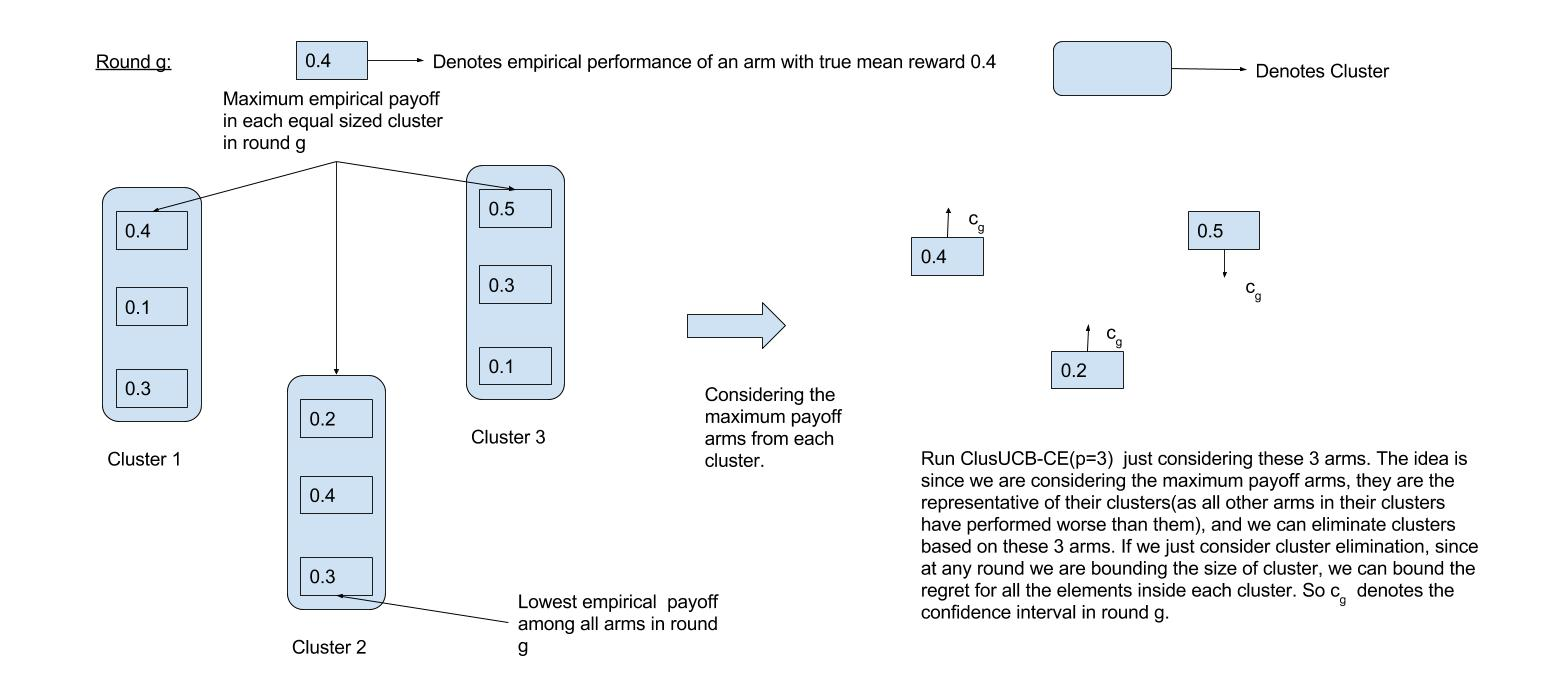
\includegraphics[scale=0.3]{img/diagCluster.jpg}
%\caption{Cluster Elimination}
%\label{Fig:ClusFig}
%\end{figure}
%
%An illustrative diagram explaining Cluster Elimination is given in \textbf{Figure \ref{Fig:ClusFig}}. A slight modification to the algorithm allows us to do cluster elimination without any arm elimination. By taking $p>1$, removing the arm elimination condition, stopping when we are just left with one cluster and pulling the $max\lbrace \hat{r}_{i}\rbrace$, where ${i}\in B_{m}$ we can achieve this. We also take $\rho_{s}\in (0,1]$ as a constant in this proof whereby in Corollary \ref{Result:Corollary:1} and \ref{Result:Corollary:2} we use the different definitions. The theoretical analysis remains same as we have always bounded the values of $\rho_{s}\in (0,1]$.
% 
%
%\begin{proof}
%Let $C_{g_{s_{k}}}=\lbrace \hat{r}_{a_{\max_{s_{k}}}} | \forall s_{k}\in S \rbrace$, that is let $C_{g_{s_{k}}}$ be the set of all arms which has the maximum estimated payoff arms from their respective clusters in the $g_{s_{k}}$-th round.  
%Let, for each sub-optimal cluster arm $a_{\max_{s_{k}}}\in C_{g_{s_{k}}}$, $g_{s_{k}}=\min{\lbrace g|\sqrt{\rho_{s}\epsilon_{g}} < \dfrac{\Delta_{a_{\max_{s_{k}}}}}{2} \rbrace}$. So, $g_{s_{k}}$ be the first round when $\sqrt{\rho_{s}\epsilon_{g_{s_{k}}}} < \dfrac{\Delta_{a_{\max_{s_{k}}}}}{2}$ where $a_{\max_{s_{k}}}\in C_{g_{s_{k}}}$ is the maximum payoff arm in cluster $s_{k}$. Here, $a_{\max_{s_{k}}}$ is called cluster arm. Here, $A_{{s_{k}}}$ denotes the arm set in the cluster $s_{k}$. Let $A_{s_{k}}^{'}=\lbrace i\in A_{s_{k}}: \Delta_{i}> b\rbrace$, $A_{s_{k}}^{''}=\lbrace i\in A_{s_{k}}: \Delta_{i} > 0\rbrace$, $A^{'}=\lbrace i\in A: \Delta_{i}> b\rbrace$ and $A^{''}=\lbrace i\in A: \Delta_{i} > 0\rbrace$.
%
%%The parameter $\rho_{s}$ is introduced just to make sure that the cluster elimination is a more aggressive elimination than arm elimination.
%\subsection*{Case a: \textit{ Some sub-optimal cluster arm $a_{max_{s_{k}}}$ is not eliminated in round $g_{s_{k}}$ or before with $* \in C_{g_{s_{k}}}$ }}
%  
%	Following the steps of Theorem \ref{Result:Theorem:1} Case $a2$, an arbitrary sub-optimal arm ${i}\in A^{'}$ can get eliminated only when the event,
%	\begin{align}
%	\hat{r}_{a_{\max_{s_{k}}}}  \le r_{a_{\max_{s_{k}}}} + c_{m_{i}} \text{ and } \label{eq:appB:armelim-casea}
% 	\hat{r}^{*}\geq  r^{*} - c_{m_{i}}
%	\end{align}
%	
%	takes place. So to bound the regret we need to bound the probability of the complementary event of these two conditions.  
%  
%  
%  Putting the value of $n_{g_{s_{k}}}=\dfrac{2\log{(\psi T\epsilon_{g_{s_{k}}}^{2})}}{\epsilon_{g_{s_{k}}}}$ in $c_{g_{s_{k}}}$ we get,
%  \begin{align*}
%  c_{g_{s_{k}}}= & \sqrt{\dfrac{\rho_{s}*\epsilon_{g_{s_{k}}}\log (\psi  T\epsilon_{g_{s_{k}}}^{2})}{2*2 \log(\psi T\epsilon_{g_{s_{k}}}^{2})}}\\
%  &=\sqrt{\dfrac{\rho_{s}\epsilon_{g_{s_{k}}}}{2}}\\
%  &=\sqrt{\rho_{s}\epsilon_{g_{s_{k}}+1}} < \dfrac{\sqrt{\rho_{s}}\Delta_{a_{\max_{s_{k}}}}}{4} < \dfrac{\Delta_{a_{\max_{s_{k}}}}}{4}
%  \end{align*}
%%  $c_{g_{s_{k}}}=\sqrt{\dfrac{\rho_{s}*\epsilon_{g_{s_{k}}}\log (\psi T\epsilon_{g_{s_{k}}}^{2})}{2*2 \log(\psi T\epsilon_{g_{s_{k}}}^{2})}}=\sqrt{\dfrac{\rho_{s}\epsilon_{g_{s_{k}}}}{2}} = \sqrt{\rho_{s}\epsilon_{g_{s_{k}}+1}} < \dfrac{\sqrt{\rho_{s}}\Delta_{a_{max_{s_{k}}}}}{4} < \dfrac{\Delta_{a_{max_{s_{k}}}}}{4} $
%
%  Again, for $a_{\max_{s_{k}}}, * \in C_{g_{s_{k}}}$, 
%  \begin{align*}
%  \hat{r}_{a_{\max_{s_{k}}}} + c_{g_{s_{k}}}\leq r_{a_{\max_{s_{k}}}} + 2c_{g_{s_{k}}} &= \hat{r}_{a_{\max_{s_{k}}}} + 4c_{g_{k}} - 2c_{g_{s_{k}}}\\
%  &< r_{a_{\max_{s_{k}}}} + \Delta_{a_{\max_{s_{k}}}} - 2c_{g_{s_{k}}}\\
%  &= r^{*} -2c_{g_{s_{k}}}\\
%  &\leq \hat{r}^{*} - c_{g_{s_{k}}}
%  \end{align*}
%   
%
%	Applying Chernoff-Hoeffding bound and considering independence of complementary of the two events in \ref{eq:appB:armelim-casea},
% 
% \begin{align*}
% \mathbb{P}\bigg\lbrace\hat{r}^{*} \leq r^{*} - c_{g_{s_{k}}}\bigg\rbrace&\leq exp(-2c_{g_{s_{k}}}^{2}n_{g_{s_{k}}})\\
% &\leq exp(-2 * \dfrac{\rho_{s}\log ( \psi T\epsilon_{g_{s_{k}}}^{2})}{2 n_{g_{s_{k}}}} *n_{g_{s_{k}}})\\
% &\leq \dfrac{1}{(\psi T\epsilon_{g_{k}}^{2})^{\rho_{s}}}
% \end{align*}
%
% 
%Similarly, $\mathbb{P}\bigg\lbrace\hat{r}_{a_{max_{s_{k}}}}\geq r_{a_{max_{s_{k}}}} + c_{g_{s_{k}}}\bigg\rbrace\leq \dfrac{1}{(\psi T\epsilon_{g_{s_{k}}}^{2})^{\rho_{s}}}$
% 
%Summing, the two up, the probability that a sub-optimal cluster arm $a_{max_{s_{k}}}\in C_{g_{s_{k}}}$ is not eliminated in $g_{s_{k}}$-th round is  $\bigg(\dfrac{2}{(\psi  T\epsilon_{g_{s_{k}}}^{2})^{\rho_{s}}}\bigg)$. 
%  Now, for each round $g_{s_{k}}$, all the elements of $C_{g_{s_{k}}}$ are the respective max payoff arms of their cluster $s_{k}$, that is all the other arms in their respective clusters have performed worse than them. Hence, since $A_{s_{k}}^{'}\supset C_{g_{s_{k}}}$, we are pulling all the surviving arms equally in each round and since clusters are fixed so we can bound the maximum probability that a sub-optimal arm ${j}\in A^{'}_{s_{k}}$  and ${j}\in s_{k}$ such that $a_{max_{s_{k}}}\in C_{g_{s_{k}}}$ is not eliminated on or before the $g_{s_{k}}$-th round by the same probability of 
%  
%  %, \forall s_{k}\in S_{g_{s_{k}}}
%\begin{align*}
%\bigg(\dfrac{2}{(\psi T\epsilon_{g_{s_{k}}}^{2})^{\rho_{s}}}\bigg)
%\end{align*}  
% 
% 
%Summing up over all arms in $s_{k}$ and bounding the regret trivially by $T\Delta_{i}$,
%\begin{align*}
%\sum_{i\in A_{s_{k}}^{'}}\bigg(\dfrac{2T\Delta_{i}}{(\psi T\epsilon_{g_{s_{k}}}^{2})^{\rho_{s}}}\bigg)
%\end{align*}
%
% 
%Summing up over all $p$ clusters and bounding the regret for each arm $i\in A_{s_{k}}^{'} $ trivially by $T\Delta_{i}$,
% \begin{align*}
% \sum_{k=1}^{p}\sum_{i\in A_{s_{k}}^{'}}\bigg(\dfrac{2T\Delta_{i}}{(\psi T\dfrac{\Delta_{i}^{4}}{16\rho_{s}^{2}})^{\rho_{s}}}\bigg) &= \sum_{i\in A^{'}}\bigg(\dfrac{2T\Delta_{i}}{(\psi  T\dfrac{\Delta_{i}^{4}}{16\rho_{s}^{2}})^{\rho_{s}}}\bigg) \\
% &\leq \sum_{i\in A^{'}}\bigg(\dfrac{2^{1+4\rho_{s}}T^{1-\rho_{s}}\rho_{s}^{2\rho_{s}}\Delta_{i}}{\psi^{\rho_{s}}\Delta_{i}^{4\rho_{s}}}\bigg)\\
% &\leq \sum_{i\in A^{'}}\bigg(\dfrac{2^{1+4\rho_{s}}\rho_{s}^{2\rho_{s}}T^{1-\rho_{s}}}{\psi^{\rho_{s}}\Delta_{i}^{4\rho_{s}-1}}\bigg)\\
% &= \sum_{i\in A^{'}}\bigg(\dfrac{C_{1}(\rho_{s})T^{1-\rho_{s}}}{\Delta_{i}^{4\rho_{s}-1}}\bigg) \text{, where } C_1(x) = \frac{2^{1+4x}x^{2x}}{\psi^{x}}
% \end{align*}
% 
%
%
%\subsection*{Case b: \textit{For each arm $i$, either ${i}$ is eliminated in round $g_{s_{k}}$ or before or there is no optimal arm ${*}$ in $C_{g_{s_{k}}}$ }}
%
%\subsubsection*{Case b1: \textit{${*}\in C_{g_{s_{k}}}$ for each arm $i \in A'$ and cluster $s_{k}$ eliminated on or before $g_{s_{k}}$} }
%	
%	Again, in the $g_{s_{k}}$-th round, the maximum total elements in the cluster $s_{k}$ can be no more than $\ell=\bigg\lceil \dfrac{K}{p}\bigg\rceil$.
% 
%Also, since we are eliminating a sub-optimal cluster arm $a_{\max_{s_{k}}}\in C_{g_{s_{k}}}$ on or before round $g_{s_{k}}$, it is pulled (along with all the other arms in that cluster) no longer than,
% \begin{align*}
% &n_{g_{s_{k}}}=\bigg\lceil\dfrac{2\log{(\psi T\epsilon_{g_{s_{k}}}^{2})}}{\epsilon_{g_{s_{k}}}}\bigg\rceil
% \end{align*}
%
%So, the total contribution of $a_{\max_{s_{k}}}$  along with all the other arms in the cluster till round $g_{s_{k}}$ is given by,
% \begin{align*}
% &\sum_{i\in A_{s_{k}}}\Delta_{i}\bigg\lceil\dfrac{2\log{(\psi T\epsilon_{g_{s_{k}}}^{2})}}{\epsilon_{g_{s_{k}}}}\bigg\rceil\\
% &\leq\sum_{i\in A_{s_{k}}^{'}}\Delta_{i}\bigg\lceil\dfrac{2\log{(\psi T(\dfrac{\Delta_{i}}{2\sqrt{\rho_{s}}})^{4})}}{(\dfrac{\Delta_{i}}{2\sqrt{\rho_{s}}})^{2}}\bigg\rceil \text{, since }\sqrt{\rho_{s}\epsilon_{g_{s_{k}}}} <\dfrac{\Delta_{a_{max_{s_{k}}}}}{2} <  \dfrac{\Delta_{i}}{2} \text{, as } {r}_{a_{max_{s_{k}}}}>{r}_{i},\forall i\in s_{k}\\
% &\leq\sum_{i\in A_{s_{k}}^{'}}\Delta_{i}\bigg(1+\dfrac{32*\rho_{s}*\log{(\psi T(\dfrac{\Delta_{i}}{2\sqrt{\rho_{s}}})^{4})}}{\Delta_{i}^{2}}\bigg)\\
% &\leq\sum_{i\in A_{s_{k}}^{'}}\Delta_{i}\bigg(1+\dfrac{32\rho_{s}\log{(\psi T\dfrac{\Delta_{i}^{4}}{16\rho_{s}^{2}})}}{\Delta_{i}^{2}}\bigg)
% \end{align*}
%
% 
%Summing over all $p$ clusters the total regret is given by,
% 
%\begin{align*}
%&\sum_{k=1}^{p}\sum_{i\in A_{s_{k}}^{'}}\Delta_{i}\bigg(1+\dfrac{32\rho_{s}\log{(\psi  T\dfrac{\Delta_{i}^{4}}{16\rho_{s}^{2}})}}{\Delta_{i}^{2}}\bigg)\\
%&\leq\sum_{i\in A^{'}}\Delta_{i}\bigg(1+\dfrac{32\rho_{s}\log{(\psi T\dfrac{\Delta_{i}^{4}}{16\rho_{s}^{2}}})}{\Delta_{i}^{2}}\bigg)
%\end{align*}
%
%
%\subsubsection*{Case b2: \textit{$s^{*}$ is eliminated by some sub-optimal cluster.} } 
%	
%	Let $C_{g}^{'}=\lbrace a_{max_{s_{k}}}\in A^{'}|\forall s_{k}\in S \rbrace$ and $C_{g}^{''}=\lbrace a_{max_{s_{k}}}\in A^{''}|\forall s_{k}\in S \rbrace$. Firstly, if conditions of case $b1$ holds then the optimal arm ${*}\in C_{g_{s_{k}}}$ will not be eliminated in round $g_{s_{k}}=g_{*}$ or it will lead to the contradiction that $r_{a_{\max_{s_{k}}}}>r^{*}$ where $a_{\max_{s_{k}}},{*}\in C_{g_{s_{k}}}$. In any round $g_{*}$, if the optimal arm ${*}$ gets eliminated then for any round from $1$ to $g_{s_{j}}$ all arms $a_{\max_{s_{j}}}\in C_{g_{s_{k}}},\forall s_{j}\neq s^{*}$ such that $g_{s_{j}}< g_{*}$ were eliminated according to assumption in Case $a$. Let, the arms surviving till $g_{*}$ round be denoted by $C_{g}^{'}$. This leaves any arm $a_{s_{b}}$ such that $g_{s_{b}}\geq g_{*}$ to still survive and eliminate arm ${*}$ in round $g_{*}$. Let, such arms that survive ${*}$ belong to $C_{g}^{''}$. Also maximal regret per step after eliminating ${*}$ is the maximal $\Delta_{a_{\max_{s_{j}}}}$ among the remaining arms ${a_{\max_{s_{j}}}}\in C_{g_{s_{j}}}$ with $g_{s_{j}}\geq g_{*}$. Hence, the maximal regret after eliminating the arm ${*}$ is upper bounded by, 
% \begin{align*}
% &\sum_{g_{*}=0}^{max_{a_{\max_{s_{j}}}\in C_{g}^{'}}g_{s_{j}}}\sum_{\substack{a_{\max_{s_{k}}}\in C_{g}^{''}: \\ g_{s_{k}} \geq g_{*}}}\bigg(\dfrac{2}{(\psi T\epsilon_{g_{s^{*}}}^{2})^{\rho_{s}}} \bigg).T\max_{\substack{a_{\max_{s_{j}}}\in C_{g}^{''}: \\ g_{s_{j}}\geq g_{*}}}{\Delta}_{a_{\max_{s_{j}}}}
% \end{align*}
%%Let $g_{s_{b}}=\min\lbrace g|\sqrt{\rho_{s}\epsilon_{g}}<\dfrac{\Delta_{a_{\max_{s_{b}}}}}{2}\rbrace$.
%But, we know that for any round $g$, elements of $C_{g}$ are the best performers in their respective clusters. So, taking that into account and $A'\supset C_{g}^{'}$ and $A''\supset C_{g}^{''}$ the regret can be bounded by,
%%\text{, since }\sqrt{\rho_{s}\epsilon_{g_{s_{j}}}} < \dfrac{\Delta_{j}}{2} <  \dfrac{\Delta_{j}}{2} \text{, as }{r}_{a_{s_{j}}}>{r}_{j},\forall j\in s_{j}
%\begin{align*}
% & \sum_{g_{*}=0}^{max_{j\in A^{'}\setminus A_{s^*}^{'}}g_{s_{j}}}\sum_{i\in A^{''}\setminus A_{s^*}^{'}:g_{s_{k}}>g_{*}}\bigg(\dfrac{2}{(\psi T\epsilon_{g_{s_{k}}}^{2})^{\rho_{s}}} \bigg).T\max_{j\in A^{''}:g_{s_{j}}\geq g_{*}}{\Delta}_{j}\\
% &\leq\sum_{g_{*}=0}^{max_{j\in A^{'}\setminus A_{s^*}^{'}}g_{s_{j}}}\sum_{i\in A^{''}\setminus A_{s^*}^{'}:g_{s_{k}}>g_{*}}\bigg(\dfrac{2}{(\psi T\epsilon_{g_{s_{k}}}^{2})^{\rho_{s}}} \bigg).T.2\sqrt{\rho_{s}\epsilon_{g_{s_{j}}}}\\
% &\leq\sum_{g_{*}=0}^{max_{j\in A^{'}\setminus A_{s^*}^{'}}g_{s_{j}}}\sum_{i\in A^{''}\setminus A_{s^*}^{'}:g_{s_{k}}>g_{*}}\bigg(\dfrac{4T^{1-\rho_{s}}}{\psi^{\rho_{s}}\epsilon_{g_{s_{k}}}^{2\rho_{s} - \frac{1}{2}}} \bigg)\\
% &\leq\sum_{i\in A^{''}\setminus A_{s^*}^{'}:g_{s_{k}}>g_{*}}\sum_{g_{*}=0}^{\min{\lbrace g_{s_{k}},g_{s_{b}}\rbrace}}\bigg(\dfrac{4T^{1-\rho_{s}}}{\psi^{\rho_{s}}2^{({2\rho_{s} - \frac{1}{2}})g_{*}}} \bigg) \\
% &\leq\sum_{i\in A^{'}\setminus A_{s^*}^{'}}\bigg(\dfrac{4T^{1-\rho_{s}}}{\psi^{\rho_{s}}2^{({2\rho_{s} - \frac{1}{2}})g_{*}}} \bigg)+\sum_{i\in A^{''}\setminus A^{'}\cup A_{s^*}^{'}}\bigg(\dfrac{4T^{1-\rho_{s}}}{\psi^{\rho_{s}}2^{({2\rho_{s} - \frac{1}{2}})g_{s_{b}}}} \bigg)\\ 
% &\leq\sum_{i\in A^{'}\setminus A_{s^*}^{'}}\bigg(\dfrac{4\rho_{s}^{2\rho_{s}}T^{1-\rho_{s}}*2^{2\rho_{s}-\frac{1}{2}}}{\psi^{\rho_{s}}\Delta_{i}^{4\rho_{s}-1}} \bigg)+\sum_{i\in A^{''}\setminus A^{'}\cup A_{s^*}^{'}}\bigg(\dfrac{4\rho_{s}^{2\rho_{s}}T^{1-\rho_{s}}*2^{2\rho_{s}-\frac{1}{2}}}{\psi^{\rho_{s}}b^{4\rho_{s}-1}} \bigg)\\
% &\leq\sum_{i\in A^{'}\setminus A_{s^*}^{'}}\bigg(\dfrac{T^{1-\rho_{s}}\rho_{s}^{2\rho_{s}}2^{2\rho_{s}+\frac{3}{2}}}{\psi^{\rho_{s}}\Delta_{i}^{4\rho_{s}-1}} \bigg)+\sum_{i\in A^{''}\setminus A^{'}\cup A_{s^*}^{'}}\bigg(\dfrac{T^{1-\rho_{s}}\rho_{s}^{2\rho_{s}}2^{2\rho_{s}+\frac{3}{2}}}{\psi^{\rho_{s}}b^{4\rho_{s}-1}} \bigg)\\
% & = \sum_{i\in A^{'}\setminus A_{s^*}^{'}}\bigg(\dfrac{C_{2}(\rho_{s})T^{1-\rho_{s}}}{\Delta_{i}^{4\rho_{s}-1}} \bigg)+\sum_{i\in A^{''}\setminus A^{'}\cup A_{s^*}^{'}}\bigg(\dfrac{C_{2}(\rho_{s})T^{1-\rho_{s}}}{b^{4\rho_{s}-1}} \bigg) \text{, where } C_2(x) = \frac{2^{2x+\frac{3}{2}}x^{2x}}{\psi^{x}}
%\end{align*}
%
%\subsubsection*{Case b3: \textit{${*}$ is not in $C_{g_{s_{k}}}$, but belongs to $B_{g_{s_{k}}}$} } 
%
%In this case the optimal arm ${*}\in s^{*}$ is not eliminated, also $s^{*}$ is not eliminated. So, for all sub-optimal arms $i$ in $A'$ which gets eliminated on or before $g_{s_{k}}$ will get pulled no less than $\bigg\lceil\dfrac{2\log{(\psi T\epsilon_{g_{s_{k}}}^{2})}}{\epsilon_{g_{s_{k}}}}\bigg\rceil$ number of times, which leads to the following bound the contribution to the expected regret, as in Case $b1$:
%
%\begin{align*}
% &\sum_{i\in A^{'}}\bigg\lbrace \Delta_{i}+\dfrac{32\rho_{s}\log{(\psi T\dfrac{\Delta_{i}^{4}}{16\rho_{s}^{2}})}}{\Delta_{i}} \bigg\rbrace 
%\end{align*} 
%
%For arms $a_i \notin s^*$, the contribution to the regret cannot be greater than that in Case $b2$. So the regret is bounded by,
%
%\begin{align*}
%\sum_{i\in A^{'}\setminus A_{s^*}^{'}}\dfrac{C_{2}(\rho_{s})T^{1-\rho_{s}}}{\Delta_{i}^{4\rho_{s}-1}} +\sum_{i\in A^{''}\setminus A^{'} \cup A_{s^*}^{'}}\dfrac{C_{2}(\rho_{s})T^{1-\rho_{s}}}{b^{4\rho_{s}-1}}
%\end{align*}
%
%
% 
%Summing up \textbf{Case a} and \textbf{Case b}, the total regret till round $g$ is given by,
%\begin{align*}
%  R_{T} \leq &  \sum_{i\in A:\Delta_{i} > b}\bigg\lbrace\underbrace{\bigg(\dfrac{C_{1}(\rho_{s})T^{1-\rho_{s}}}{\Delta_{i}^{4\rho_{s}-1}}\bigg)}_{\text{case a}} + \underbrace{\bigg(2\Delta_{i}+\dfrac{64\rho_{s}\log{(\psi T\dfrac{\Delta_{i}^{4}}{16\rho_{s}^{2}})}}{\Delta_{i}} }_{\text{case b1+b3}} \bigg\rbrace
%  \\&+ \underbrace{\sum_{i\in A\setminus A_{s^*}: \Delta_{i} > b}\bigg(\dfrac{2C_{2}(\rho_{s})T^{1-\rho_{s}}}{\Delta_{i}^{4\rho_{s} -1}} \bigg)}_{\text{case b2}} \bigg\rbrace  + \underbrace{\sum_{i\in A\setminus A_{s^*}:0 < \Delta_{i}\leq b}\bigg(\dfrac{2C_{2}(\rho_{s})T^{1-\rho_{s}}}{\Delta_{i}^{4\rho_{s} -1}} \bigg)}_{\text{case b2}}  + max_{i\in A:\Delta_{i}\leq b}\Delta_{i}T
%\end{align*}
%\end{proof}


\section{Proof of Corollary 1}
\label{App:Proof:Corollary:1}
\begin{proof}
Here we take $\psi=\dfrac{T}{196 \log(K)}$, $\rho_{a}=\dfrac{1}{2}$ and $\rho_{s}=\dfrac{1}{2}$. Taking into account Theorem \ref{Result:Theorem:1} below for all $b\geq \sqrt{\dfrac{K}{14 T}}$

\begin{align*}
&\E [R_{T}]\leq 
\sum\limits_{\substack{i\in A_{s^{*}},\\\Delta_{i} > b}}\bigg\lbrace \dfrac{C_1(\rho_{a})T^{1-\rho_{a}}}{\Delta_{i}^{4\rho_{a}-1}} + \Delta_{i}
 + \frac{32\rho_{a}\log{(\psi T\dfrac{\Delta_{i}^{4}}{16\rho_{a}^{2}})}}{\Delta_{i}} \bigg\rbrace
 + \! \! \sum\limits_{\substack{i\in A,\\\Delta_{i} > b}} \bigg\lbrace 2\Delta_{i}+
\dfrac{C_1(\rho_{s})T^{1-\rho_{s}}}{\Delta_{i}^{4\rho_{s}-1}} \\
&+ \frac{32\rho_{a}\log{(\psi T\dfrac{\Delta_{i}^{4}}{16\rho_{a}^{2}})}}{\Delta_{i}} 
+ \dfrac{32\rho_{s}\log{(\psi T\dfrac{\Delta_{i}^{4}}{16\rho_{s}^{2}})}}{\Delta_{i}}\bigg\rbrace 
%%%
+ \sum\limits_{\substack{i\in A_{s^{*}},\\ \Delta_{i} > b}} 
\frac{C_2(\rho_{a})T^{1-\rho_{a}}}{\Delta_{i}^{4\rho_{a}-1}}
+\sum\limits_{\substack{i\in A_{s^{*}},\\0 < \Delta_{i}\leq b}}\frac{C_2(\rho_a)T^{1-\rho_{a}}}{b^{4\rho_{a} -1}}\\ 
 & + \sum_{i\in A\setminus A_{s^*}: \Delta_{i} > b}\dfrac{2C_{2}(\rho_{s})T^{1-\rho_{s}}}{\Delta_{i}^{4\rho_{s}-1}} +\sum_{i\in A\setminus A_{s^*}: 0 < \Delta_{i} \leq b}\dfrac{2C_{2}(\rho_{s})T^{1-\rho_{s}}}{b^{4\rho_{s}-1}} +
 \!+\! \max\limits_{i:\Delta_{i}\leq b}\Delta_{i}T
\end{align*}

and putting the parameter values in the above Theorem \ref{Result:Theorem:1} result,
	\begin{align*}
	\sum_{i\in A_{s^{*}}:\Delta_{i} > b}\bigg(\dfrac{T^{1-\rho_{a}}\rho_{a}^{2\rho_{a}}2^{1+4\rho_{a}}}{\psi^{\rho_{a}}\Delta_{i}^{4\rho_{a}-1}} \bigg)= \sum_{i\in A_{s^{*}}:\Delta_{i} > b}\bigg(\dfrac{T^{1-\frac{1}{2}}\frac{1}{2}^{2*\frac{1}{2}}2^{1+4*\frac{1}{2}}}{(\frac{T}{196 \log (K)})^{\frac{1}{2}}\Delta_{i}^{4*\frac{1}{2}-1}} \bigg)=\sum_{i\in A_{s^{*}}:\Delta_{i} > b}\dfrac{56\sqrt{\log (K)}}{\Delta_{i}}
	\end{align*}
	
	Similarly for the term,
	\begin{align*}
	\sum_{i\in A:\Delta_{i} > b}\bigg(\dfrac{T^{1-\rho_{s}}\rho_{a}^{2\rho_{s}}2^{1+4\rho_{s}}}{\psi^{\rho_{s}}\Delta_{i}^{4\rho_{s}-1}} \bigg) = \sum_{i\in A:\Delta_{i} > b}\dfrac{56\sqrt{\log (K)}}{\Delta_{i}}
	\end{align*}		
			
	
	For the term involving arm pulls,
	\begin{align*}
	\sum_{i\in A:\Delta_{i} > b}\dfrac{32\rho_{s}\log{(\psi T\dfrac{\Delta_{i}^{4}}{16\rho_{s}^{2}})}}{\Delta_{i}}=\sum_{i\in A:\Delta_{i} > b}\dfrac{16\log{(T^{2}\dfrac{\Delta_{i}^{4}}{784\log (K)})}}{\Delta_{i}}\approx \sum_{i\in A:\Delta_{i} > b}\dfrac{32\log{(T\dfrac{\Delta_{i}^{2}}{\sqrt{\log (K)}})}}{\Delta_{i}}
	\end{align*}		
	 Similarly the term, 
	
	\begin{align*}
	\sum_{i\in A:\Delta_{i} > b}\dfrac{32\rho_{a}\log{(\psi T\dfrac{\Delta_{i}^{4}}{16\rho_{a}^{2}})}}{\Delta_{i}}\approx \sum_{i\in A:\Delta_{i} > b}\dfrac{32\log{(T\dfrac{\Delta_{i}^{2}}{\sqrt{\log (K)}})}}{\Delta_{i}}
	\end{align*}		 
	 

	Lastly we can bound the error terms as, 
	\begin{align*}
	\sum\limits_{i\in A_{s^{*}}:0 < \Delta_{i}\leq b}\bigg(\dfrac{T^{1-\rho_{a}}\rho_{a}^{2\rho_{a}}2^{2\rho_{a}+\frac{3}{2}}}{\psi^{\rho_{a}}\Delta_{i}^{4\rho_{a}-1}} \bigg)= \sum\limits_{i\in A_{s^{*}}:0 < \Delta_{i}\leq b}\dfrac{40\sqrt{\log (K)}}{\Delta_{i}}
	\end{align*}
	
	
	Similarly for the term,
	
	\begin{align*}
	\sum_{i\in A\setminus A_{s^*}: 0 < \Delta_{i} \leq b}\bigg(\dfrac{T^{1-\rho_{s}}\rho_{s}^{2\rho_{s}}2^{2\rho_{s}+\frac{3}{2}}}{(\psi^{\rho_{s}})\Delta_{i}^{4\rho_{s} -1}} \bigg)=\sum_{i\in A\setminus A_{s^*}: 0 < \Delta_{i} \leq b}\dfrac{40\sqrt{\log (K)}}{\Delta_{i}}
	\end{align*}	 
		
	
	So, the total gap dependent regret bound for using both arm and cluster elimination comes of as
	\begin{align*}
	& \sum_{i\in A_{s^{*}}:\Delta_{i} > b}\bigg\lbrace \dfrac{56\sqrt{\log (K)}}{\Delta_{i}} + \Delta_{i} + \dfrac{32\log{(T\dfrac{\Delta_{i}^{2}}{\sqrt{\log (K)}})}}{\Delta_{i}} \bigg\rbrace + \sum_{i\in A:\Delta_{i} > b}\bigg\lbrace\dfrac{56\sqrt{\log (K)}}{\Delta_{i}} + 2\Delta_{i} + \dfrac{64\log{(T\dfrac{\Delta_{i}^{2}}{\sqrt{\log (K)}})}}{\Delta_{i}}\bigg\rbrace\\
	 & + \sum\limits_{i\in A_{s^{*}}:\Delta_{i} > b}\dfrac{40\sqrt{\log (K)}}{\Delta_{i}} + \sum\limits_{i\in A_{s^{*}}:0< \Delta_{i} <\leq b}\dfrac{40\sqrt{\log (K)}}{\Delta_{i}}
	+ \sum\limits_{i\in A\setminus A_{s^{*}}:\Delta_{i} > b}\dfrac{80\sqrt{\log (K)}}{\Delta_{i}}\\
	& + \sum\limits_{i\in A\setminus A \cup A_{s^{*}} :0 < \Delta_{i}\leq b}\dfrac{80\sqrt{\log (K)}}{\Delta_{i}} + \max\limits_{i\in A:\Delta_{i}\leq b}\Delta_{i}T 
	\end{align*}
\end{proof}




\section{Proof of Corollary 2}
\label{App:Proof:Corollary:2}
\begin{proof}
As stated in \citet{auer2010ucb}, we can have a bound on regret of the order of $\sqrt{KT\log K}$ in non-stochastic setting. This is shown in Exp4\cite{auer2002nonstochastic} algorithm. Also we know from \citet{bubeck2011pure} that the function $x\in [0,1]\mapsto x\exp(-Cx^2)$ is  decreasing on $\left[\dfrac{1}{\sqrt{2C}},1\right ]$ for any $C>0$. So, taking $C=\left\lfloor \dfrac{14 T}{K}\right\rfloor$ and similarly, by choosing  $\Delta_{i}=\Delta=\sqrt{\dfrac{K\log K}{T}}>\sqrt{\dfrac{K}{14 T}}$ for all ${i:i\neq *}\in A$, in the bound of UCB1\cite{auer2002finite} we get,

\begin{align*}
\sum_{i:r_{i}<r^{*}}const \dfrac{\log T}{\Delta_{i}}=\dfrac{\sqrt{KT}\log T}{\sqrt{\log K}}
\end{align*}
So, this bound is worse than the non-stochastic setting and is clearly improvable and an upper bound regret of $\sqrt{KT}$ is possible as shown in \citet{audibert2009minimax} for MOSS which is consistent with the lower bound as proposed by Mannor and Tsitsiklis\cite{mannor2004sample}.

	Hence, we take $b\approx\sqrt{\dfrac{K\log K}{T}} > \sqrt{\dfrac{K}{14 T}}$(the minimum value for $b$), $\psi=\dfrac{T}{196 \log K}$, $\rho_{a}=\dfrac{1}{2}$ and $\rho_{s}=\dfrac{1}{2}$.
	
	Taking into account Theorem \ref{Result:Theorem:1} below, 
	
\begin{align*}
&\E [R_{T}]\leq 
\sum\limits_{\substack{i\in A_{s^{*}},\\\Delta_{i} > b}}\bigg\lbrace \dfrac{C_1(\rho_{a})T^{1-\rho_{a}}}{\Delta_{i}^{4\rho_{a}-1}} + \Delta_{i}
 + \frac{32\rho_{a}\log{(\psi T\dfrac{\Delta_{i}^{4}}{16\rho_{a}^{2}})}}{\Delta_{i}} \bigg\rbrace
 + \! \! \sum\limits_{\substack{i\in A,\\\Delta_{i} > b}} \bigg\lbrace 2\Delta_{i}+
\dfrac{C_1(\rho_{s})T^{1-\rho_{s}}}{\Delta_{i}^{4\rho_{s}-1}} \\
&+ \frac{32\rho_{a}\log{(\psi T\dfrac{\Delta_{i}^{4}}{16\rho_{a}^{2}})}}{\Delta_{i}} 
+ \dfrac{32\rho_{s}\log{(\psi T\dfrac{\Delta_{i}^{4}}{16\rho_{s}^{2}})}}{\Delta_{i}}\bigg\rbrace 
%%%
+ \sum\limits_{\substack{i\in A_{s^{*}},\\ \Delta_{i} > b}} 
\frac{C_2(\rho_{a})T^{1-\rho_{a}}}{\Delta_{i}^{4\rho_{a}-1}}
+\sum\limits_{\substack{i\in A_{s^{*}},\\0 < \Delta_{i}\leq b}}\frac{C_2(\rho_a)T^{1-\rho_{a}}}{b^{4\rho_{a} -1}}\\ 
 & + \sum_{i\in A\setminus A_{s^*}: \Delta_{i} > b}\dfrac{2C_{2}(\rho_{s})T^{1-\rho_{s}}}{\Delta_{i}^{4\rho_{s}-1}} +\sum_{i\in A\setminus A_{s^*}: 0 < \Delta_{i} \leq b}\dfrac{2C_{2}(\rho_{s})T^{1-\rho_{s}}}{b^{4\rho_{s}-1}} +
 \!+\! \max\limits_{i:\Delta_{i}\leq b}\Delta_{i}T
\end{align*}

and putting the parameter values in the above Theorem \ref{Result:Theorem:1} result,	
	
	\begin{align*}
	\sum_{i\in A_{s^{*}}:\Delta_{i} > b}\bigg(\dfrac{T^{1-\rho_{a}}\rho_{a}^{2\rho_{a}}2^{1+4\rho_{a}}}{\psi^{\rho_{a}}\Delta_{i}^{4\rho_{a}-1}} \bigg)=& \bigg(K\dfrac{T^{1-\frac{1}{2}}\frac{1}{2}^{2\frac{1}{2}}2^{1+4\frac{1}{2}}}{p(\frac{T}{196 \log K})^{\frac{1}{2}}\Delta_{i}^{4\frac{1}{2}-1}} \bigg)=56\dfrac{\sqrt{KT}}{p}
	\end{align*}		
	 Similarly, for the term, 
	 \begin{align*}
	 \sum_{i\in A:\Delta_{i} > b}\bigg(\dfrac{T^{1-\rho_{s}}\rho_{s}^{2\rho_{s}}2^{1+4\rho_{s}}}{\psi^{\rho_{s}}\Delta_{i}^{4\rho_{s}-1}} \bigg) = 56\sqrt{KT}
	 \end{align*}
	 
	
	For the term regarding number of pulls,
	\begin{align*}
	\sum_{i\in A:\Delta_{i} > b}\dfrac{32\rho_{s}\log{(\psi T\dfrac{\Delta_{i}^{4}}{16\rho_{s}^{2}})}}{\Delta_{i}} &= \dfrac{32K\sqrt{T}\frac{1}{2}\log{(T^{2}\dfrac{K^{4}(\log K)^{2}}{784 T^{2}\log K})}}{\sqrt{K\log K}} \leq  \dfrac{32\sqrt{KT}\log{(\frac{1}{28} K^{2}(\sqrt{\log K}))}}{\sqrt{\log K}}\\
	&\leq 64\sqrt{KT\log K} + \dfrac{32\sqrt{KT}\log{(\sqrt{\log K})}}{\sqrt{\log K}}
	\end{align*}		
	
	Similarly for the term,
	\begin{align*}
	\sum_{i\in A:\Delta_{i} > b}\dfrac{32\rho_{a}\log{(\psi T\dfrac{\Delta_{i}^{4}}{16\rho_{a}^{2}})}}{\Delta_{i}} \leq 64\sqrt{KT\log K} + \dfrac{32\sqrt{KT}\log{(\sqrt{\log K})}}{\sqrt{\log K}}
	\end{align*}		
	
 	Lastly we can bound the error terms as, 
	\begin{align*}
	\sum\limits_{i\in A_{s^{*}}:0\leq\Delta_{i}\leq b}\bigg(\dfrac{T^{1-\rho_{a}}\rho_{a}^{2\rho_{a}}2^{2\rho_{a}+\frac{3}{2}}}{\psi^{\rho_{a}}\Delta_{i}^{4\rho_{a}-1}} \bigg)=\dfrac{K}{p}\bigg(\dfrac{T^{1-\frac{1}{2}}\frac{1}{2}^{2\frac{1}{2}}2^{2\frac{1}{2}+\frac{3}{2}}}{{(\frac{T}{196 \log K})^{\frac{1}{2}}}{(\Delta_{i})^{4*\frac{1}{2}-1}}} \bigg) < \dfrac{150 \sqrt{KT\log K} }{p}
	\end{align*}	 	
 	Similarly for the term,
 	\begin{align*}
 	\sum_{i\in A\setminus A_{s^*}: \Delta_{i} > b}\bigg(\dfrac{T^{1-\rho_{s}}\rho_{s}^{2\rho_{s}}2^{2\rho_{s}+\frac{3}{2}}}{(\psi^{\rho_{s}})\Delta_{i}^{4\rho_{s} -1}} \bigg) < 150(K-\dfrac{K}{p})\sqrt{\dfrac{T}{K\log K}}
	\end{align*} 	
	Also, for all $b\geq \sqrt{\dfrac{K}{14T}}$,
	\begin{align*}
 	\sum_{i\in A\setminus A_{s^*}: 0 < \Delta_{i} \leq b}\bigg(\dfrac{T^{1-\rho_{s}}\rho_{s}^{2\rho_{s}}2^{2\rho_{s}+\frac{3}{2}}}{(\psi^{\rho_{s}})b^{4\rho_{s} -1}} \bigg) < 150(K-\dfrac{K}{p})\sqrt{\dfrac{T\log K}{K}}
	\end{align*} 	
	
	Now, $K-\dfrac{K}{p}= K\left( \dfrac{p-1}{p} \right) < K\left(  \dfrac{\frac{K}{\log K}+1-1}{\frac{K}{\log K}+1 }\right) < \dfrac{K^2}{K+\log K}$. So, after putting the value of $p=\left\lceil \dfrac{K}{\log K} \right\rceil$, we get,
	
	\begin{align*}
	\E[R_{T}]\leq & 56\dfrac{\sqrt{T}\log K}{\sqrt{K}} + 64\dfrac{\sqrt{T}\log K}{\sqrt{K}} + \dfrac{32\sqrt{T\log K}\log{(\log K)}}{\sqrt{K}} + 56\sqrt{KT} + 128\sqrt{KT\log K}\\
	& + \dfrac{64\sqrt{KT}\log{(\log K)}}{\sqrt{\log K}} + \dfrac{150 \sqrt{T}\log K^{\frac{3}{2}} }{\sqrt{K}} + \dfrac{150 \sqrt{T}\log K}{\sqrt{K}} + 300 \dfrac{K}{K+\log K}\sqrt{KT\log K} + 300 \dfrac{K}{K+\log K}\sqrt{KT}\\ 
	\end{align*}
 	
	So, the total bound for using both arm and cluster elimination cannot be worse than,
	
	\begin{align*}
	\E[R_{T}]\leq & 270\dfrac{\sqrt{T}\log K}{\sqrt{K}} + \dfrac{32\sqrt{T\log K}\log{(\log K)}}{\sqrt{K}} + 56\sqrt{KT} + 128\sqrt{KT\log K}\\
	& + \dfrac{64\sqrt{KT}\log{(\log K)}}{\sqrt{\log K}} + \dfrac{150 \sqrt{T}\log K^{\frac{3}{2}} }{\sqrt{K}} + 300 \dfrac{K}{K+\log K}\sqrt{KT\log K} + 300 \dfrac{K}{K+\log K}\sqrt{KT}\\ 
	\end{align*}		
\end{proof}

\section{Why Clustering?}
\label{App:E}

In this section we want to specify the apparent use of clustering. The error bounds are shown in Table \ref{App:E:table:3}.


%The regret bound for both arm elimination and pulls and error bound when a sub-optimal arm or a sub-optimal cluster eliminates ${*}$ or $s^{*}$ is given in Table \ref{App:E:table:2}, \ref{App:E:table:3}respectively.
 
%\begin{table}
%\caption{Regret Bound on Arm Elimination and Pulls}
%\label{App:E:table:2}
%\begin{center}
%\begin{tabular}{p{1.4cm}p{10.2cm}p{3.5cm}}
%\multicolumn{1}{c}{\bf Elim Type} &\multicolumn{1}{c}{\bf Regret Bound on Arm Elimination and Pulls} &\multicolumn{1}{c}{\bf Remarks} \\
%\hline \\
%Only Arm Elimination (ClusUCB-AE)	& \begin{align*}\sum_{i\in A:\Delta_{i} > b}\bigg\lbrace\underbrace{\bigg(\dfrac{C_{1}(\rho_{a})T^{1-\rho_{a}}}{\Delta_{i}^{4\rho_{a}-1}}\bigg)}_{\text{Case a1, Proposition \ref{proofTheorem:Prop:1}}} + \underbrace{\bigg(\Delta_{i}+ \dfrac{32\rho_{a}\log{(\psi  T\dfrac{\Delta_{i}^{4}}{16\rho_{a}^{2}})}}{\Delta_{i}}\bigg)}_{\text{case b1, Proposition \ref{proofTheorem:Prop:1}}}\bigg\rbrace \end{align*} & For $\rho_{a}=\frac{1}{4}$ and $\psi=K^{2}T$ this gives $ 2\sqrt{KT} + 32\sqrt{KT\log K} + \dfrac{16\log(\log K)}{\sqrt{\log K}}$. Hence the order is given by $O(\sqrt{KT\log K})$.\\
%%$\sum_{i\in A:\Delta_{i}\geq b}\bigg\lbrace\underbrace{\bigg(\dfrac{2^{1+4\rho_{a}}\rho_{a}^{2\rho_{a}}T^{1-\rho_{a}}}{(\psi)^{\rho_{a}}\Delta_{i}^{4\rho_{a}-1}}\bigg)}_{\text{Case a1, Proposition \ref{proofTheorem:Prop:1}}} + \underbrace{\bigg(\Delta_{i}+ \dfrac{32\rho_{a}\log{(\psi  T\dfrac{\Delta_{i}^{4}}{16\rho_{a}^{2}})}}{\Delta_{i}}\bigg)}_{\text{case b1, Proposition \ref{proofTheorem:Prop:1}}}\bigg\rbrace$
%\hline\\
%Only Cluster Elimination (ClusUCB-CE)	&\begin{align*} \sum_{i\in A:\Delta_{i} > b}\bigg\lbrace\underbrace{\bigg(\dfrac{C_{1}(\rho_{s})T^{1-\rho_{s}}}{\Delta_{i}^{4\rho_{s}-1}}\bigg)}_{\text{Case a, Proposition \ref{proofTheorem:Prop:2}}} +  \underbrace{\bigg(2\Delta_{i} +\dfrac{64\rho_{s}\log{(\psi T\dfrac{\Delta_{i}^{4}}{16\rho_{s}^{2}})}}{\Delta_{i}}\bigg)}_{\text{Case b1+b3, Proposition \ref{proofTheorem:Prop:2}}}\bigg\rbrace \end{align*} & With $\rho_{s}=\frac{1}{4}$ and  $\psi=K^{2}T$ this gives $ 2\sqrt{KT} + 64\sqrt{KT\log K} + \dfrac{32\log(\log K)}{\sqrt{\log K}}$. Hence, this is larger bound than using only arm elimination though the order is same $O(\sqrt{KT\log K})$.\\
%%$ \sum_{i\in A:\Delta_{i}\geq b}\bigg\lbrace\underbrace{\bigg(\dfrac{2^{2+4\rho_{s}}\rho_{s}^{2\rho_{s}}T^{1-\rho_{s}}}{(\psi)^{\rho_{s}}\Delta_{i}^{4\rho_{s}-1}}\bigg)}_{\text{Case a1+a2, Proposition \ref{proofTheorem:Prop:2}}} +  \underbrace{\bigg(\Delta_{i} +\dfrac{32\rho_{s}\log{(\psi T\dfrac{\Delta_{i}^{4}}{16\rho_{s}^{2}})}}{\Delta_{i}}\bigg)}_{\text{Case b1, Proposition \ref{proofTheorem:Prop:2}}}\bigg\rbrace$
%\hline\\
%Arm \& Cluster Elimination (ClusUCB) 	&\begin{align*} \sum_{i\in A_{s^{*}}:\Delta_{i} > b} \underbrace{\bigg(\dfrac{C_{1}(\rho_{a})T^{1-\rho_{a}}}{\Delta_{i}^{4\rho_{a}-1}}\bigg)}_{\text{Case a1, Arm Elim, Theorem \ref{Result:Theorem:1}}} +  \sum_{i\in A:\Delta_{i} > b} \bigg\lbrace\underbrace{\bigg(\dfrac{C_{2}(\rho_{s})T^{1-\rho_{s}}}{\Delta_{i}^{4\rho_{s}-1}}\bigg)}_{\text{Case a2, Clus Elim, Theorem \ref{Result:Theorem:1}}} 
% \\ + \underbrace{\bigg(\Delta_{i}+\dfrac{64\rho_{a}\log{(\psi T\dfrac{\Delta_{i}^{4}}{16\rho_{a}^{2}})}}{\Delta_{i}}\bigg)}_{\text{Case b1+b4, Arm Elim, Theorem \ref{Result:Theorem:1}}} +\underbrace{\bigg(\Delta_{i}+\dfrac{32\rho_{s}\log{(\psi T\dfrac{\Delta_{i}^{4}}{16\rho_{s}^{2}})}}{\Delta_{i}}\bigg)}_{\text{Case b1, Clus Elim, Theorem \ref{Result:Theorem:1}}}\bigg\rbrace\end{align*} & With $\rho_{a}=\frac{1}{4}$,$\rho_{s}=\frac{1}{2}$ and $\psi=K^{2}T$ this gives $\bigg\lbrace \dfrac{2\sqrt{KT}}{p} + 4\sqrt{\dfrac{T}{K\log K}} + 128\sqrt{KT\log K} + \dfrac{64\log(\log K)}{\sqrt{\log K}} \bigg\rbrace$. This is larger than the previous $2$ bounds though the order is same $O(\sqrt{KT\log K})$.
%%$\sum_{i\in A:\Delta_{i}\geq b} \bigg\lbrace \underbrace{\bigg(\dfrac{2^{1+4\rho_{a}}\rho_{a}^{2\rho_{a}}T^{1-\rho_{a}}}{(\psi)^{\rho_{a}}\Delta_{i}^{4\rho_{a}-1}}\bigg)}_{\text{Case a, Arm Elim, Theorem \ref{Result:Theorem:1}}} + \underbrace{\bigg(\dfrac{2^{2+4\rho_{s}}\rho_{s}^{2\rho_{s}}T^{1-\rho_{s}}}{(\psi)^{\rho_{s}}\Delta_{i}^{4\rho_{s}-1}}\bigg)}_{\text{Case a, Clus Elim, Theorem \ref{Result:Theorem:1}}} $   $+ \underbrace{\bigg(\Delta_{i}+\dfrac{32\rho_{a}\log{(\psi T\dfrac{\Delta_{i}^{4}}{16\rho_{a}^{2}})}}{\Delta_{i}}\bigg)}_{\text{Case b1, Arm Elim, Theorem \ref{Result:Theorem:1}}} +\underbrace{\bigg(\Delta_{i}+\dfrac{32\rho_{s}\log{(\psi T\dfrac{\Delta_{i}^{4}}{16\rho_{s}^{2}})}}{\Delta_{i}}\bigg)}_{\text{Case b1, Clus Elim, Theorem \ref{Result:Theorem:1}}}\bigg\rbrace$
%\end{tabular}
%\end{center}
%\end{table}

\begin{table}
\caption{Error Bound}
\label{App:E:table:3}
\begin{center}
\begin{tabular}{p{1.4cm}p{10.3cm}p{3.5cm}}
\multicolumn{1}{c}{\bf Elim Type} &\multicolumn{1}{c}{\bf Error Bound} &\multicolumn{1}{c}{\bf Remarks} \\
\hline \\
Only Arm Elimination (EClusUCB-AE)	& \begin{align*}\underbrace{\sum_{i\in A:\Delta_{i} > b}\bigg(\dfrac{C_{2}(\rho_{a})T^{1-\rho_{a}}}{\Delta_{i}^{4\rho_{a} -1}} \bigg)}_{\text{Case b2, Proposition \ref{proofTheorem:Prop:1}}} + \underbrace{\sum_{i\in A:0 < \Delta_{i}\leq b}\bigg( \dfrac{C_{2}(\rho_{a})T^{1-\rho_{a}}}{b^{4\rho_{a} -1}} \bigg)}_{\text{Case b2, Proposition \ref{proofTheorem:Prop:1}}}\end{align*}  & With $\rho_{a}=\frac{1}{2},$ and $\psi=\frac{T}{196 \log K}$ this gives $150\sqrt{KT}+150\sqrt{KT\log K}$. Hence, this has an order of $O(\sqrt{KT\log K})$.\\
%$\underbrace{\sum_{i\in A:\Delta_{i}\geq b}\bigg(\dfrac{T^{1-\rho_{a}}\rho_{a}^{2\rho_{a}}2^{2\rho_{a}+\frac{3}{2}}}{(\psi)^{\rho_{a}}\Delta_{i}^{4\rho_{a} -1}} \bigg)}_{\text{Case b2, Proposition \ref{proofTheorem:Prop:1}}} + \underbrace{\sum_{i\in A:0\leq\Delta_{i}\leq b}\bigg( \dfrac{T^{1-\rho_{a}}\rho_{a}^{2\rho_{a}}2^{2\rho_{a}+\frac{3}{2}}}{(\psi)^{\rho_{a}}b^{4\rho_{a} -1}} \bigg)}_{\text{Case b2, Proposition \ref{proofTheorem:Prop:1}}}$
\hline\\
%%%%%%%%%%%%%%%%%%%%%%%%%%%%%%%%%%%%%%%%%%%%%%%%%%%%%%%%%%%%%%%%%%%%%%%%
%Only Cluster Elimination	 (ClusUCB-CE) & \begin{align*} \underbrace{\sum_{i\in A\setminus A_{s^*}:\Delta_{i} > b}\bigg(\dfrac{2C_{2}(\rho_{s})T^{1-\rho_{s}}}{\Delta_{i}^{4\rho_{s} -1}} \bigg)}_{\text{Case b2+b3, Proposition \ref{proofTheorem:Prop:2}}} +\underbrace{\sum_{i\in A\setminus A_{s^*}:0\leq\Delta_{i}\leq b}\bigg(\dfrac{2C_{2}(\rho_{s})T^{1-\rho_{s}}}{b^{4\rho_{s} -1}} \bigg)}_{\text{Case b2+b3, Proposition \ref{proofTheorem:Prop:2}}} \end{align*} & With $\rho_{s}=\frac{1}{2}$ and $\psi=K^{2}T$ this gives $4\sqrt{KT}+4\sqrt{KT\log K}$. This is same as the bound using only arm elimination and has an order of $O(\sqrt{KT\log K})$.\\
%\hline\\
%%%%%%%%%%%%%%%%%%%%%%%%%%%%%%%%%%%%%%%%%%%%%%%%%%%%%%%%%%%%%%%%%%%%%%%%%%
Arm \& Cluster Elimination (EClusUCB) 	& \begin{align*}  \underbrace{\sum_{i\in A_{s^{*}}:\Delta_{i} > b}\bigg(\dfrac{C_{2}(\rho_{a})T^{1-\rho_{a}}}{\Delta_{i}^{4\rho_{a}-1}} \bigg)+ \sum_{i\in A_{s^{*}}:0\leq\Delta_{i}\leq b}\bigg(\dfrac{C_{2}(\rho_{a})T^{1-\rho_{a}}}{b^{4\rho_{a} -1}} \bigg)}_{\text{Case b2, Arm Elim, Theorem \ref{Result:Theorem:1}}}\\   
 + \underbrace{\sum_{i\in A\setminus A_{s^*}:\Delta_{i} > b}\bigg(\dfrac{2C_{2}(\rho_{s})T^{1-\rho_{s}}}{\Delta_{i}^{4\rho_{s}-1}} \bigg)+ \sum_{i\in A\setminus A_{s^*}:0\leq\Delta_{i}\leq b}\bigg(\dfrac{2C_{2}(\rho_{s})T^{1-\rho_{s}}}{b^{4\rho_{s} -1}} \bigg)}_{\text{Case b3+b4, Clus Elim, Theorem \ref{Result:Theorem:1}}} \end{align*} & With $\rho_{a}=\frac{1}{2}$, $\rho_{s}=\frac{1}{2}, p=\lceil \frac{K}{\log K}\rceil$ and $\psi=\frac{T}{196 \log K}$ this gives $\frac{150 \sqrt{T}\log K^{\frac{3}{2}} }{\sqrt{K}} + \frac{150 \sqrt{T}\log K}{\sqrt{K}} + 300 \frac{K}{K+\log K}\sqrt{KT\log K} + 300 \frac{K}{K+\log K}\sqrt{KT}$. So we can reduce the error bound to $O(\frac{K}{K+\log K}\sqrt{KT\log K})$.\\
\hline
\end{tabular}
\end{center}	
\end{table}
% From Table \ref{App:E:table:2} we can see that from the definition of $\rho_{s},\rho_{a}$ we can have a regret bound for jointly doing the arm and cluster elimination of the same order as doing arm elimination or cluster elimination alone. 
 
While looking at the error terms in Table~\ref{App:E:table:3}, we see that using just arm elimination (EClusUCB-AE) the elimination error bound is more than using both arm and cluster  elimination simultaneously (EClusUCB). 
%From Table \ref{App:E:table:3}, we can see that the error term for using both arm and cluster elimination can become low depending on how we choose $p$ since $|A_{s^{*}}|\leq \lceil\frac{A}{p}\rceil$ and in Corollary \ref{Result:Corollary:2} we proved that taking $p=\big\lceil \frac{K}{\log K} \big\rceil$ reduces the elimination error bound.
 
 
%%%%%%%%%%%%%%%%%%%%
%Table for Regret Bounds  
%%%%%%%%%%%%%%%%%%%% 
 
%\begin{figure}
%\centering
%  \begin{tabular}{c}
%  \begin{subfigure}{0.45\textwidth}
% \tabl{c}{\scalebox{0.8}{\begin{tikzpicture}
%      \begin{axis}[
%	xlabel={timestep},
%	ylabel={Cumulative regret},
%       clip mode=individual,grid,grid style={gray!30},
%  legend style={at={(0.5,-0.2)},anchor=north, legend columns=2} ]
%      % UCB
%\addplot table[x index=0,y index=1,col sep=tab,each nth point={10}] {results/Expt4/clUCB1comp_subsampled.txt};
%\addplot table[x index=0,y index=1,col sep=tab,each nth point={10}] {results/Expt4/clUCB2comp_subsampled.txt};
%\addplot table[x index=0,y index=1,col sep=tab,each nth point={10}] {results/Expt4/clUCB3comp_subsampled.txt};
%\addplot table[x index=0,y index=1,col sep=tab,each nth point={10}] {results/Expt4/MOSScomp_subsampled.txt};
%\addplot table[x index=0,y index=1,col sep=tab,each nth point={10}] {results/Expt4/clUCB4comp_subsampled.txt};
%\addplot table[x index=0,y index=1,col sep=tab,each nth point={10}] {results/Expt4/clUCB5comp_subsampled.txt};
%      \legend{ClusUCB(1A),ClusUCB(4B),ClusUCB(10B),MOSS,ClusUCB(5S),ClusUCB(10S)}
%      %\legend{ClusUCB (NC, p=1),ClusUCB (C, p=4),ClusUCB(C, p=10) ,MOSS, ClusUCB(C, p=5, NAE), ClusUCB(C, p=10, NAE)}
%      %\legend{ClusUCB(1,A),ClusUCB(4,B),ClusUCB(10,B), MOSS,ClusUCB(5,S), ClusUCB(10,A)}
%      \end{axis}
%      \end{tikzpicture}}\\}
%			\caption{Experiment $4$: ClusUCB for various $p$. ClusUCB(1A)= $\lbrace$ p=$1$,Only Arm Elimination $\rbrace$, ClusUCB(4B)=$\lbrace$ p=$4$, Both Arm and Cluster Elimination$\rbrace$, ClusUCB(5S)=$\lbrace$ p=$5$, Only Cluster Elimination$\rbrace$. }
%  \label{Fig:variousClus}
%  \end{subfigure}
%  \end{tabular}
%
%\end{figure}

%\end{remark}

%\section{Regret Bound Table}
%\label{App:F}
%The regret upper bound of various algorithms are given in Table \ref{sample-table}.
%\begin{table}
%\caption{Regret Upper Bound of Algorithms}
%\label{sample-table}
%\begin{center}
%\begin{tabular}{l|l}
%\multicolumn{1}{c}{\bf Algorithm}  &\multicolumn{1}{c}{\bf Regret Upper Bound} \\
%\hline \\
%UCB1         &\hspace*{5em}$\min\bigg\lbrace O(\sqrt{KT\log T}) ,O\bigg(\dfrac{K\log T}{\Delta}\bigg)\bigg\rbrace$ \\
%%UCB2         &\hspace*{5em}$O\bigg(K\bigg(\dfrac{(1 + \epsilon(\alpha)) log(T)}{2\Delta} + C(\alpha)\bigg)\bigg)$, $0<\alpha<1$ \\
%$\epsilon_{n}$-greedy         &\hspace*{5em}$O\bigg(\dfrac{K\Delta\log T}{d^{2}}\bigg)$, $0<d<\Delta$ \\
%%EXP3             &\hspace*{5em}$O\bigg(S \sqrt{KT \log(KT)}\bigg)$, where $S$ is the hardness of the problem \\
%%UCB($\delta$)	&\hspace*{5em}$O\bigg(\dfrac{16K}{\Delta}\log\big(\dfrac{2K}{\Delta\delta}\big)\bigg)$ , where $\delta$ is the error probability\\
%UCB-Improved             &\hspace*{5em}$\min\bigg\lbrace O\bigg(\sqrt{KT\log K}\bigg), O\bigg(\dfrac{K\log (T\Delta^{2})}{\Delta}\bigg)\bigg\rbrace$ \\
%MOSS				&\hspace*{5em}$\min\bigg\lbrace O\bigg(\sqrt{KT}\bigg), O\bigg(\dfrac{K\log(T\Delta^{2}/K)}{\Delta}\bigg) \bigg \rbrace$\\
%%KL-UCB         &\hspace*{5em}$O\bigg(K\bigg(\dfrac{\Delta \log(T)(1 + \epsilon)}{d(r_{i}, r^{*} )} + \log(\log(T)) + \dfrac{(\epsilon)}{T^{\beta(\epsilon)}}\bigg)\bigg)$, where $\epsilon > 0$ and $d(r_{i}, r^{*})>2\Delta_{i}^{2}$\\
%UCB-Clustered             &\hspace*{5em}$\min\bigg\lbrace O\bigg(\sqrt{KT\log K}\bigg),O\bigg(\dfrac{K\log\big (\dfrac{T\Delta^{2}}{\sqrt{\log (KT)}}\big)}{\Delta}\bigg)\bigg\rbrace$\\
%\end{tabular}
%\end{center}
%\end{table}

%%%%%%%%%%%%%%%%%%%%%%%%%%%%%%%%
%Moved to Main paper
%%%%%%%%%%%%%%%%%%%%%%%%%%%%%%%%

%\section{Efficient Clustered UCB}

%\begin{algorithm}[t]
%\caption{EClusUCB}
%\label{alg:eclusucb}
%\begin{algorithmic}
%\State {\bf Input:} Number of clusters $p$, time horizon $T$, exploration parameters $\rho_a$, $\rho_s$ and $\psi$.
%\State {\bf Initialization:} Set $m:=0$, $B_{0}:=A$, $S_0 = S$, $\epsilon_{0}:=1$, $M=\big \lfloor \dfrac{1}{2}\log_{2} \dfrac{7T}{K}\big\rfloor$, $n_{0}=\bigg\lceil\dfrac{2\log{(\psi T\epsilon_{0}^{2})}}{\epsilon_{0}}\bigg\rceil$ and  $N_{0}=K*n_{0}$.
%\State Create a partition $S_0$ of the arms at random into $p$ clusters of size up to $\ell=\bigg\lceil \dfrac{K}{p} \bigg\rceil$ each.
%\State Pull each arm once
%\For{$t=K+1,..,T$}	
%\State Pull arm $i$ in $B_m$ such that $\max_{i\in B_{m}}\bigg\lbrace \hat{r}_{i} + \sqrt{\dfrac{\rho_{s}\log{(\psi T\epsilon_{m}^{2})}}{2 n_{i}}} \bigg\rbrace$
%\State $t:=t+1$
%\ArmElim
%\State For each cluster $s_k \in S_{m}$, delete arm ${i}\in s_{k}$ from $B_{m}$ if
%\begin{align*}
%\hat{r}_{i} + \sqrt{\dfrac{\rho_{a}\log{(\psi T\epsilon_{m}^{2})}}{2 n_{i}}}  < \max_{{j}\in s_{k}}\bigg\lbrace\hat{r}_{j} -\sqrt{\dfrac{\rho_{a}\log{(\psi T\epsilon_{m}^{2})}}{2 n_{j}}} \bigg\rbrace
%\end{align*}
% where $\rho_{a}=\dfrac{1}{w_{m}}$ and remove all such arms from $B_{m}$.
%\EndArmElim
%\ClusElim
%\State Delete cluster $s_{k}\in S_{m}$ and remove all arms $i\in s_{k}$ from $B_{m}$ if 
%\begin{align*}
% \max_{{i}\in s_{k}}\bigg\lbrace\hat{r}_{i} + \sqrt{\dfrac{\rho_{s}\log{(\psi T\epsilon_{m}^{2})}}{2 n_{i}}}\bigg\rbrace 
% < \max_{{j}\in B_{m}} \bigg\lbrace\hat{r}_{j} - \sqrt{\dfrac{\rho_{s} \log{(\psi T\epsilon_{m}^{2})}}{2 n_{j}}}\bigg\rbrace.
%\end{align*}
%  and remove all such arms in the cluster $s_{k}$ from $B_{m}$ to obtain $B_{m+1}$.
%\EndClusElim
%
%\If{$t\geq N_{m}$ and $m\leq M$}
%\ResParam
%\State $\epsilon_{m+1}:=\dfrac{\epsilon_{m}}{2}$\vspace{0.5ex}
%\State $B_{m+1}:=B_{m}$
%\State $n_{m}:=\bigg\lceil\dfrac{2\log{(\psi T\epsilon_{m}^{2})}}{\epsilon_{m}}\bigg\rceil$
%\State $N_{m}:=t+|B_{m}| * n_{m}$
%\State $m:=m+1$
%\EndResParam
%\State \hspace*{2em} $\ell_{m+1}:=\min\lbrace 2\ell_{m}, K\rbrace$
%\State \hspace*{2em} $w_{m+1}:=2w_{m}$
%\State Stop if $|B_{m}|=1$ and pull ${i}\in B_{m}$ till $T$ is reached.
%\EndIf
%\EndFor
%\end{algorithmic}
%\end{algorithm}
%
%In ClusUCB we modified UCB-Improved to reduce early exploration and do faster elimination of sub-optimal arms and clusters with the help of clustering. With careful choosing of exploration regulatory factor $\psi$ and elimination parameters $\rho_{a}$ and $\rho_{s}$ we were able to bring down the cumulative regret compared to UCB-Improved. One of the principal dis-advantage that still remain is that ClusUCB is a round based algorithm which samples all remaining arms equally in each round (still less compared to UCB-Improved). In this section, we introduce a further modification,  as shown in Algorithm \ref{alg:eclusucb} called Efficient Clustered UCB hence referred to as EClusUCB where we introduce the idea of optimistic greedy sampling. A similar idea was also used in \cite{liu2016modification} which they used to modify the UCB-Improved algorithm. We further modify the idea by introducing clustering and arm elimination parameters. Also we use different exploration regulatory factor and we come up with a cumulative regret bound whereas  \cite{liu2016modification} only gives simple regret bound. In optimistic greedy sampling we only sample the arm with the highest upper confidence bound in each timestep. Also in EClusUCB we check arm elimination condition and cluster elimination condition in every timestep and update parameters when a round is complete. Drawing from the idea of UCB-Improved, we divide each round into $|B_{m}|n_{m}$ timesteps so that each surviving arms can be allocated atmost $n_{m}$ pulls. In the next section we analyze the regret of EClusUCB. 


%%%%%%%%%%%%%%%%%%%%%%%%%%%%%%%%%%%%%%%%%%%%%%%%%%%%%%%%%
% Proof of EClusUCB
%%%%%%%%%%%%%%%%%%%%%%%%%%%%%%%%%%%%%%%%%%%%%%%%%%%%%%%%%
%\section{Proof of Theorem 2}
%\label{App:EClusUCB}
%
%\begin{theorem}[\textbf{\textit{Regret bound}}]
%\label{Result:Theorem:2}
%The regret $R_T$ of EClusUCB satisfies
%\begin{align*}
%&\E [R_{T}]\leq 
%\sum\limits_{\substack{i\in A_{s^{*}},\\\Delta_{i} > b}}\bigg\lbrace \dfrac{C_1(\rho_{a})T^{1-\rho_{a}}}{\Delta_{i}^{4\rho_{a}-1}} + \Delta_{i}
% + \frac{32\rho_{a}\log{(\psi T\dfrac{\Delta_{i}^{4}}{16\rho_{a}^{2}})}}{\Delta_{i}} \bigg\rbrace
% + \! \! \sum\limits_{\substack{i\in A,\\\Delta_{i} > b}} \bigg\lbrace 2\Delta_{i}+
%\dfrac{C_1(\rho_{s})T^{1-\rho_{s}}}{\Delta_{i}^{4\rho_{s}-1}} \\
%&+ \frac{32\rho_{a}\log{(\psi T\dfrac{\Delta_{i}^{4}}{16\rho_{a}^{2}})}}{\Delta_{i}} 
%+ \dfrac{32\rho_{s}\log{(\psi T\dfrac{\Delta_{i}^{4}}{16\rho_{s}^{2}})}}{\Delta_{i}}\bigg\rbrace
%+ \sum\limits_{\substack{i\in A_{s^{*}},\\ \Delta_{i} > b}} 
%\frac{C_2(\rho_{a})T^{1-\rho_{a}}}{\Delta_{i}^{4\rho_{a}-1}}
%+\sum\limits_{\substack{i\in A_{s^{*}},\\0 < \Delta_{i}\leq b}}\frac{C_2(\rho_a)T^{1-\rho_{a}}}{b^{4\rho_{a} -1}}\\ 
%%%%%%%%
%%&+ \!\sum\limits_{\substack{i\in A,\\ \Delta_{i} > b}}\! \! \dfrac{C_2(\rho_{s})T^{1-\rho_{s}}}{\Delta_{i}^{4\rho_{s}-1}}
%% + \!\sum\limits_{\substack{i\in A,\\0 < \Delta_{i}\leq b}}\! \! \dfrac{C_2(\rho_{s})T^{1-\rho_{s}}}{b^{4\rho_{s} -1}}  \\
%&+ \sum_{\substack{i\in A\setminus A_{s^*}:\\\Delta_{i}> b}}\dfrac{2C_{2}(\rho_{s})T^{1-\rho_{s}}}{\Delta_{i}^{4\rho_{s}-1}} +\sum_{\substack{i\in A \setminus A_{s^*}:\\ 0 < \Delta_{i} \leq b}}\dfrac{2C_{2}(\rho_{s})T^{1-\rho_{s}}}{b^{4\rho_{s}-1}}\\
%& \!+\! \max\limits_{i:\Delta_{i}\leq b}\Delta_{i}T, 
%\end{align*}
%
%where $b\geq \sqrt{\frac{K}{14 T}}$, $C_1(x) = \frac{2^{1+4x}x^{2x}}{\psi^{x}}$, $C_2(x) = \frac{2^{2x+\frac{3}{2}}x^{2x}}{\psi^{x}}$ and $A_{s^{*}}$ is the subset of arms in cluster $s^{*}$ containing optimal arm $a^{*}$.
%%, $\rho_{a}=\dfrac{1}{2},\rho_{s}=\dfrac{1}{2}$ and $\psi=K^{2}T$.
%\end{theorem}
%
%We can see from the result of this theorem that the regret upper bound for EClusUCB is same as ClusUCB. Also we can specialize the result of this Theorem \ref{Result:Theorem:2} using Corollary \ref{Result:Corollary:1} and \ref{Result:Corollary:2} to achieve a similar bound as for Theorem \ref{Result:Theorem:1}.
%
%\begin{proof}
%\label{sec:proofTheorem1}
%%$\Delta_{i}^{'}=r_{a_{\max_{s_{k}}}} - r_{i}$ such that $a_{i}\in s_{k}$,
%% m_{i}^{'}=\min{\lbrace m|\sqrt{\rho_{a}\epsilon_{m}} < \frac{\Delta_{i}^{'}}{2} \rbrace}
%Let $A^{'}=\lbrace i \in A,\Delta_{i}> b\rbrace$,  $A^{''}=\lbrace i \in A, \Delta_{i} > 0\rbrace$, $A^{'}_{s_{k}}=\lbrace i \in A_{s_{k}},\Delta_{i}> b\rbrace$ and $A^{''}_{s_{k}}=\lbrace i \in A_{s_{k}}, \Delta_{i} > 0 \rbrace$. $C_{g}$ is the cluster set containing max payoff arm from each cluster in $g$-th round. The arm having the highest payoff in a cluster $s_{k}$ is denote by $a_{\max_{s_{k}}}$. Let for each sub-optimal arm ${i}\in A$, $m_{i}=\min{\lbrace m|\sqrt{\rho_{a}\epsilon_{m}} < \frac{\Delta_{i}}{2} \rbrace}$ and let for each cluster $s_{k}\in S$, $g_{s_{k}}=\min{\lbrace g|\sqrt{\rho_{s}\epsilon_{g}} < \frac{\Delta_{a_{\max_{s_{k}}}}}{2} \rbrace}$. 
%Let $\check{A}=\lbrace {i}\in A^{'} | {i}\in s_{k} , \forall s_{k}\in S \rbrace$. Also $z_{i}$ denotes total number of times an arm $i$ has been pulled from $1$ to $(t-1)$-th timestep. In the $m$-th round, $n_{m}$ denotes the number of pulls allocated to the surviving arms in $B_{m}$. The analysis proceeds by considering the contribution to the regret in each of the following cases:
%
%\textbf{Case a:} \textit{Some sub-optimal arm ${i}$ is not eliminated in round $\max(m_{i},g_{s_{k}})$ or before, with the optimal arm ${*}\in C_{\max(m_{i},g_{s_{k}})}$.}
%
%We consider an arbitrary sub-optimal arm ${i}$ and analyze the contribution to the regret when $i$ is not eliminated in the following exhaustive sub-cases:\\
%\textbf{Case a1:} \textit{In round $\max(m_{i},g_{s_{k}})$, ${i} \in s^{*}$.}
%
%This case is similar to Case a1, Theorem \ref{Result:Theorem:1}. Let $c_{i}=\sqrt{\dfrac{\rho_{a}\log{(\psi T\epsilon_{m}^{2})}}{2 z_{i}}}$. For an arm to get eliminated it must satisfy the following condition,
%\begin{align}
%\hat{r}_{i}  \le r_{i} + c_{i} \text{ and } 
%\hat{r}^{*}\geq  r^{*} - c^{*}, \label{eq:armelim-casea2}
%\end{align}
%
%Since each round now consist of $|B_{m}|n_{m}$ timesteps and since at every timestep the arm elimination condition is being checked, following a parallel arguement as in Case a1, Theorem $\ref{Result:Theorem:1}$ we can show that when $z_{i} = n_{m_{i}}$ then \\ $c_{i} \leq c_{m_{i}} \leq \sqrt{\dfrac{\rho_{a}\log{(\psi T\epsilon_{m}^{2})}}{2 n_{m_{i}}}} = \sqrt{\rho_{a}\epsilon_{m_{i}+1}} < \frac{\Delta_{i}}{4}$, since $z_{i} =  n_{m_{i}}=\frac{2\log{(\psi T\epsilon_{m_{i}}^{2})}}{\epsilon_{m_{i}}}$ and $\rho_{a}\in (0,1]$.
%
%Subsequently following the steps of Case a1, Theorem \ref{Result:Theorem:1} we can upper bound the probability of the complementary of the events in \ref{eq:armelim-casea2} and show that the probability that a sub-optimal arm ${i}$ is not eliminated in any round on or before $m_{i}$ is bounded above by  $\bigg(\frac{2}{(\psi T\epsilon_{m_{i}}^{2})^{\rho_{a}}}\bigg)$.
%
%%%%%%%%%%%%%%%%%%%%%%%%%%%%%%%%%%%%%%%%%%%%%%%%%%%%%%%%%%%%%%%%%%%%%%%%%%%%%%%%%%%%%%%%%%%%%%%%   
%\textbf{Case a2:} \textit{In round $\max(m_{i},g_{s_{k}})$, ${i} \in s_k$ for some $s_k \ne s^{*}$.}
%
%Let $c_{a_{\max_{s_{k}}}}=\sqrt{\dfrac{\rho_{s}\log{(\psi T\epsilon_{m}^{2})}}{2 z_{a_{max_{s_{k}}}}}}$ and $z_{a_{max_{s_{k}}}}$ is the number of times $a_{max_{s_{k}}}$ has been pulled. Following a parallel argument like in Case $a1$, we have to bound the following two events of arm $a_{\max_{s_{k}}}$ not getting eliminated on or before $g_{s_{k}}$-th round,
%\begin{align*}
%  \hat{r}_{a_{\max_{s_{k}}}} \geq r_{a_{\max_{s_{k}}}} +c_{a_{\max_{s_{k}}}} \text{ and } \hat{r}^{*} \leq r^{*} -c^{*}  
%\end{align*} 
%
%As we argued in previous case, since cluster elimination condition being verified in each timestep, the above two conditions are possible when $z_{a_{max_{s_{k}}}} = n_{g_{s_{k}}}$. We can prove using Chernoff-Hoeffding bounds and considering independence of events mentioned above, that for $c_{a_{\max_{s_{k}}}} \leq c_{g_{s_{k}}} \leq \sqrt{\frac{\rho_{s} \log (\psi T\epsilon_{g_{s_{k}}}^{2})}{2 n_{g_{s_{k}}}}}$ and  $n_{g_{s_{k}}}=\frac{2\log{(\psi T\epsilon_{g_{s_{k}}}^{2})}}{\epsilon_{g_{s_{k}}}}$ the probability of the above two events is bounded by $\bigg(\dfrac{2}{(\psi  T\epsilon_{g_{s_{k}}}^{2})^{\rho_{s}}}\bigg)$.
%%Summing, the two up, the probability that a sub-optimal cluster arm $a_{\max_{s_{k}}}\in C_{g_{s_{k}}}$ is not eliminated
%  Now, for any round $g_{s_{k}}$, all the elements of $C_{\max(m_{i},g_{s_{k}})}$ are the respective maximum payoff arms of their cluster $s_{k}, \forall s_{k}\in S$, and since clusters are fixed so we can bound the maximum probability that a sub-optimal arm ${i}\in A^{'}$  and ${i}\in s_{k}$ such that $a_{\max_{s_{k}}}\in C_{g_{s_{k}}}$ is not eliminated on or before the $g_{s_{k}}$-th round by the same probability as above. 
%
%Summing up over all $p$ clusters and bounding the regret for each arm $i\in A_{s_{k}}^{'}$ trivially by $T\Delta_{i}$ and following the steps of Case a2, Theorem \ref{Result:Theorem:1}, we can show that the regret for not eliminating clusters on or before round $g_{s_{k}}$ is upper bounded by,
%
%\begin{align*}
%\sum_{i\in A^{'}}\frac{C_{1}(\rho_{s})T^{1-\rho_{s}}}{\Delta_{i}^{4\rho_{s}-1}}
%\end{align*}
%
%
%
%Summing the bounds in Cases $a1-a2$ and observing that the bounds in the aforementioned cases hold for any round $C_{\max \lbrace m_i,g_{s_k}\rbrace}$, we obtain the following contribution to the expected regret from Case a:
%   %Taking summation of the events mentioned above($a1$-$a4$) gives us an upper bound on the regret given that the optimal arm $a^{*}$ is still surviving, 
%\begin{align*}
%&\sum_{i\in A_{s^*}} \frac{C_{1}(\rho_{a})T^{1-\rho_{a}}}{\Delta_{i}^{4\rho_{a}-1}} + \sum_{i\in A^{'}}\bigg(\frac{C_{1}(\rho_{s})T^{1-\rho_{s}}}{\Delta_{i}^{4\rho_{s}-1}}\bigg)
%\end{align*}
%
%
%
%%%%%%%%%%%%%%%%%%%%%%%%%%%%%%%%%%%%%%%%%%%%%%%%%%%%%%%%%%%%%%%%%%%%%%%%%%%%%%%%%%%%%%%%%%%%%
%\textbf{Case b:} \textit{For each arm $i$, either ${i}$ is eliminated in round $\max (m_{i},g_{s_{k}})$ or before or there is no optimal arm ${*}$ in $C_{\max(m_{i},g_{s_{k}})}$.} \\
%
%\textbf{Case b1:} \textit{${*}\in C_{\max(m_{i},g_{s_{k}})}$ for each arm $i \in A'$ and cluster $s_k \in \check A$.} 
%
%%\todos{define $\check A$}
%
%The condition in the case description above implies the following: \\
%\begin{inparaenum}[\bfseries (i)]
%\item each sub-optimal arm ${i}\in A^{'}$ is  eliminated on or before $\max (m_{i},g_{s_{k}})$ and hence  pulled not more than $z_{i}$ number of times. But according to the condition of Case a1, $z_{i} < n_{m_{i}}$ number of times.\\
%\item each sub-optimal cluster $s_k \in \check A$ is eliminated on or before $\max (m_{i},g_{s_{k}})$ and hence  pulled not more than $n_{a_{\max_{s_{k}}}}$ number of times. But again according to condition Case a2,  $z_{a_{\max_{s_{k}}}} < n_{g_{s_{k}}}$ number of times.
%\end{inparaenum}
%
%Hence, following the same steps as in Case b1, Theorem \ref{Result:Theorem:1}, the maximum regret suffered due to pulling of a sub-optimal arm or a sub-optimal cluster is no more than the following:
% \begin{align*}
%\sum_{i\in A^{'}}\!\bigg[ 2\Delta_{i}+\dfrac{32(\rho_{a}\log{(\psi T\dfrac{\Delta_{i}^{4}}{16\rho_{a}^{2}})} + \rho_{s}\log{(\psi T\dfrac{\Delta_{i}^{4}}{16\rho_{s}^{2}})})}{\Delta_{i}} \bigg]
% \end{align*}
%
% 
%%%%%%%%%%%%%%%%%%%%%%%%%%%%%%%%%%%%%%%%%%%%%%%%%%%%%%%%%%%%%%%%%%%%%%%%%%%%%%%%%%%%%%%%%%%%%%%%   
%%\textbf{Case b2:} \textit{Optimal arm $a^{*}$ is eliminated by a sub-optimal arm.}\\
%  %
%	%This, can happen in $3$ ways,
%%\newline
%\textbf{Case b2:} \textit{${*}$ is eliminated by some sub-optimal arm in $s^*$} \\
%%In this case, we are concerned with the arm elimination condition only. 
%Optimal arm $a^*$ can get eliminated by some sub-optimal arm $i$ only if arm elimination condition holds, i.e., 
%\begin{align*}
%\hat r_{i} - c_{i} > \hat{r}^{*}+ c^{*},
%\end{align*}
%where, as mentioned before, $c_{i} \leq c_{m_{i}} \leq \sqrt{\frac{\rho_{a}\log (\psi T\epsilon_{m_{i}}^{2})}{2 n_{m_{i}}}}$.
%From analysis in Case $a1$, notice that, if \eqref{eq:armelim-casea2} holds in conjunction with the above, arm $i$ gets eliminated. Also, recall from Case $a1$ that the events complementary to \eqref{eq:armelim-casea2} have low-probability and can be upper bounded by $\frac{2}{(\psi  T\epsilon_{m_{*}}^{2})^{\rho_{a}}}$. Moreover, a sub-optimal arm that eliminates $*$ has to survive until round $m_*$. In other words, 
%all arms ${j}\in s^{*}$ such that $m_{j} < m_{*}$ are eliminated on or before $m_*$ (this corresponds to case b1). 
%Let, the arms surviving till $m_{*}$ round be denoted by $A^{'}_{s^{*}}$. This leaves any arm $a_{b}$ such that $m_{b}\geq m_{*} $ to still survive and eliminate arm ${*}$ in round $m_{*}$. Let, such arms that survive ${*}$ belong to $A^{''}_{s^{*}}$. Also maximal regret per step after eliminating ${*}$ is the maximal $\Delta_{j}$ among the remaining arms in $A^{''}_{s^{*}}$ with $m_{j}\geq m_{*}$.  Let $m_{b}=\min\lbrace m|\sqrt{\rho_{a}\epsilon_{m}}<\frac{\Delta_{b}}{2}\rbrace$. Let $C_2(x) = \frac{2^{2x+\frac{3}{2}}x^{2x}}{\psi^{x}}$. Hence, the maximal regret after eliminating the arm ${*}$ is upper bounded by, 
%\begin{align*}
%&\sum_{m_{*}=0}^{max_{j\in A^{'}_{s^{*}}}m_{j}}\sum_{\substack{i\in A^{''}_{s^{*}}: \\ m_{i}\geq m_{*}}}\bigg(\dfrac{2}{(\psi  T\epsilon_{m_{*}}^{2})^{\rho_{a}}} \bigg).T\max_{\substack{j\in A^{''}_{s^{*}}: \\ m_{j}\geq m_{*}}}{\Delta}_{j}\\
%\end{align*}
%Therefore, following the similar steps as in Case b2, Theorem \ref{Result:Theorem:1}, we can show that the above regret is upper bounded by,
%\begin{align*}
%\sum_{i\in A^{'}_{s^{*}}}\dfrac{ C_{2}(\rho_{a}) T^{1-\rho_{a}}}{\Delta_{i}^{4\rho_{a}-1}} +\sum_{i\in A^{''}_{s^{*}}\setminus A^{'}_{s^{*}}}\dfrac{C_{2(\rho_{a})}T^{1-\rho_{a}}}{b^{4\rho_{a}-1}}
%\end{align*}
%
%
%
%%%%%%%%%%%%%%%%%%%%%%%%%%%%%%%%%%%%%%%%%%%%%%%%%%%%%%%%%%%%%%%%%%%%%%%%%%%%%%%%%%%%%%%%%%%%%%%%   
%\textbf{Case b3:} \textit{$s^{*}$ is eliminated by some sub-optimal cluster.} 
%
%Let $C_{g}^{'}=\lbrace a_{max_{s_{k}}}\in A^{'}|\forall s_{k}\in S \rbrace$ and $C_{g}^{''}=\lbrace a_{max_{s_{k}}}\in A^{''}|\forall s_{k}\in S \rbrace$. A sub-optimal cluster $s_k$ will eliminate $s^*$ in round $g_*$ only if the cluster elimination condition of Algorithm \ref{alg:eclusucb} holds, which is the following when ${*}\in C_{g_{*}}$:
%\begin{align}
%\hat r_{a_{\max_{s_k}}} - c_{a_{\max_{s_k}}} > \hat{r}^{*}+ c^{*}.
%\label{eq:caseb3-ecluselim}
%\end{align}
%Notice that when ${*}\notin C_{g_{*}}$, since $r_{a_{max_{s_{k}}}}>r^{*}$, the inequality in \eqref{eq:caseb3-ecluselim} has to hold for cluster $s_k$ to eliminate $s^*$.
%As in case $b2$, the probability that a given sub-optimal cluster $s_k$ eliminates $s^*$ is upper bounded by  $\frac{2}{(\psi T\epsilon_{g_{s^{*}}}^{2})^{\rho_{s}}}$ and all sub-optimal clusters with $g_{s_{j}}< g_{*}$ are eliminated before round $g_*$. 
%
%This leaves any arm $a_{\max_{s_{b}}}$ such that $g_{s_{b}}\geq g_{*}$ to still survive and eliminate arm ${*}$ in round $g_{*}$. Let, such arms that survive ${*}$ belong to $C_{g}^{''}$. Hence, following the same way as case $b2$,  the maximal regret after eliminating ${*}$ is,
% \begin{align*}
% \!\!\sum_{g_{*}=0}^{\max\limits_{a_{\max_{s_{j}}}\in C_{g}^{'}}g_{s_{j}}}\!\!\!\!\!\sum_{\substack{\scriptsize a_{\max_{s_{k}}}\in C_{g}^{''}: \\ g_{s_{k}} \geq g_{*}}}\bigg(\dfrac{2}{(\psi T\epsilon_{g_{s^{*}}}^{2})^{\rho_{s}}} \bigg)T\max_{\substack{a_{\max_{s_{j}}}\in C_{g}^{''}: \\ g_{s_{j}}\geq g_{*}}}{\Delta}_{a_{\max_{s_{j}}}}
% \end{align*}
%Using $A'\supset C_{g}^{'}$ and $A''\supset C_{g}^{''}$, we can bound the regret contribution from this case in a similar manner as Case $b2$ as follows:
%
%\begin{align*}
% &\!\!\sum_{i\in A^{'}\setminus A_{s^*}^{'}}\frac{T^{1-\rho_{s}}\rho_{s}^{2\rho_{s}}2^{2\rho_{s}+\frac{3}{2}}}{\psi^{\rho_{s}}\Delta_{i}^{4\rho_{s}-1}} 
% \!+\!\!\!\sum_{i\in A^{''}\setminus A^{'}\cup A_{s^*}^{'}}\!\!\!\!\frac{T^{1-\rho_{s}}\rho_{s}^{2\rho_{s}}2^{2\rho_{s}+\frac{3}{2}}}{\psi^{\rho_{s}}b^{4\rho_{s}-1}} \\
% & = \sum_{i\in A^{'}\setminus A_{s^*}^{'}}\frac{C_{2}(\rho_{s})T^{1-\rho_{s}}}{\Delta_{i}^{4\rho_{s}-1}} +\sum_{i\in A^{''}\setminus A^{'}\cup A_{s^*}^{'}}\frac{C_{2}(\rho_{s})T^{1-\rho_{s}}}{b^{4\rho_{s}-1}} 
%\end{align*}
%
%
%
%%%%%%%%%%%%%%%%%%%%%%%%%%%%%%%%%%%%%%%%%%%%%%%%%%%%%%%%%%%%%%%%%%%%%%%%%%%%%%%%%%%%%%%%%%%%%%%%   
% 
%\textbf{Case b4:} \textit{${*}$ is not in $C_{\max(m_{i},g_{s_{k}})}$, but belongs to $B_{\max(m_{i},g_{s_{k}})}$.}
%
%In this case the optimal arm ${*}\in s^{*}$ is not eliminated, also $s^{*}$ is not eliminated. So, for all sub-optimal arms $i$ in $A_{s^*}^{'}$ which gets eliminated on or before $\max \lbrace m_{i},g_{s_{k}} \rbrace$ will get pulled no less than $z_{i} < \bigg\lceil\dfrac{2\log{(\psi T\epsilon_{m_{i}}^{2})}}{\epsilon_{m_{i}}}\bigg\rceil$ number of times, which leads to the following bound the contribution to the expected regret, as in Case $b1$:
%% 
%% \begin{align*}
%%  &\sum_{i\in A^{'}}\Delta_{i}\bigg\lceil\dfrac{2\log{(\psi T\epsilon_{m_{i}}^{2})}}{\epsilon_{m_{i}}}\bigg\rceil
%% \end{align*}
%% Since $a^{*}$ is definitely in $B_{\max(m_{i},g_{s_{k}})}$ then following the same way as Case $b1$ we can show that can be no worse than,
%\begin{align*}
% &\sum_{i\in A_{s^*}^{'}}\bigg\lbrace \Delta_{i}+\dfrac{32\rho_{a}\log{(\psi T\dfrac{\Delta_{i}^{4}}{16\rho_{a}^{2}})}}{\Delta_{i}} \bigg\rbrace 
%\end{align*} 
%
%For arms $a_i \notin s^*$, the contribution to the regret cannot be greater than that in Case $b3$. So the regret is bounded by,
%
%\begin{align*}
%\sum_{i\in A^{'}\setminus A_{s^*}^{'}}\dfrac{C_{2}(\rho_{s})T^{1-\rho_{s}}}{\Delta_{i}^{4\rho_{s}-1}} +\sum_{i\in A^{''}\setminus A^{'} \cup A_{s^*}^{'}}\dfrac{C_{2}(\rho_{s})T^{1-\rho_{s}}}{b^{4\rho_{s}-1}}
%\end{align*}
%The main claim follows by summing the contributions to the expected regret from each of the cases above.
%\end{proof}

%%%%%%%%%%%%%%%%%%%%%%%%%%%%%%%%%%%%%%%%%%%%%%%%%%%%%%%%%%%%


\section{Proof of Theorem~\ref{Result:Theorem:3}}
\label{App:SR_EClusUCB}
\begin{theorem}
\label{Result:Theorem:3}

For every $0<\eta <1$ and $\gamma > 1$, there exists $\tau$ such that for all $T>\tau$ the simple regret of EClusUCB is upper bounded by,
\begin{align*}
SR_{EClusUCB} \leq 4\log_{2}\dfrac{14 T}{K}\gamma \sum_{i=1}^{K} \Delta_{i} \exp(-\dfrac{c_{0}\sqrt{e}}{4}) \bigg\lbrace K^{\frac{3}{2} +2\rho_{a}} \bigg(\dfrac{\log (\psi T )}{T^{\frac{3}{2}}(\psi T^2)^{\rho_{a}}}\bigg) + K^{\frac{3}{2} +2\rho_{s}} \bigg(\dfrac{\log (\psi T )}{T^{\frac{3}{2}}(\psi T^2)^{\rho_{s}}}\bigg) \bigg\rbrace
\end{align*}

with probability at least $1-\eta$, where $c_{0}>0$ is a constant.

\end{theorem}


\begin{proof}
We follow the same steps as in Theorem 2, \cite{liu2016modification}. First we will state the two facts used by this proof.

\begin{enumerate}
\item \emph{Fact 1:} From Theorem \ref{Result:Theorem:1} we know that the probability of elimination of a sub-optimal arm in the $\max(m_{i},g_{s_{k}})$ round is $\bigg(\dfrac{2}{(\psi T\epsilon_{m_{i}}^{2})^{\rho_{a}}}\bigg)$ and of a sub-optimal cluster is $\bigg(\dfrac{2}{(\psi  T\epsilon_{g_{s_{k}}}^{2})^{\rho_{s}}}\bigg)$.
\item \emph{Fact 2:} From \citet{tolpin2012mcts} we know that, for every $0<\eta <1$ and $\gamma > 1$, there exists $\tau$ such that for all $T>\tau$ the probability of a sub-optimal arm $i$ being sampled in the $m$-th round is bounded by $Q_{m}\leq 2\gamma \exp(-c_{m}\dfrac{\sqrt{T}}{2})$, where $c_{m}=\dfrac{c_{0}}{2^{m}}$.
\end{enumerate}

We start with an upper bound on the number of plays $\delta_{\max(m_{i},g_{s_{k}})}$ in the $\max(m_{i},g_{s_{k}})$-th round divided by the total number of plays $T$. We know  from Fact $1$  that the total number of arms surviving in the $\max(m_{i},g_{s_{k}})$-th arm is 

\begin{align*}
|B_{\max(m_{i},g_{s_{k}})}|\leq\bigg(\dfrac{2K}{(\psi T\epsilon_{m_{i}}^{2})^{\rho_{a}}}\bigg) + \bigg(\dfrac{2K}{(\psi  T\epsilon_{g_{s_{k}}}^{2})^{\rho_{s}}}\bigg)
\end{align*}     

Again in EClusUCB, we know that the number of pulls allocated for each surviving arm $i$ in the $\max(m_{i},g_{s_{k}})$-th round is $n_{\max(m_{i},g_{s_{k}})}=\dfrac{2\log (\psi T \epsilon_{\max(m_{i},g_{s_{k}})}^{2})}{\epsilon_{\max(m_{i},g_{s_{k}})}}$. Therefore, the proportion of plays $\delta_{\max(m_{i},g_{s_{k}})}$ in the $\max(m_{i},g_{s_{k}})$-th round can be written as,

\begin{align*}
\delta_{\max(m_{i},g_{s_{k}})}=\dfrac{(|B_{\max(m_{i},g_{s_{k}})}|.n_{\max(m_{i},g_{s_{k}})})}{T} &\leq \bigg(\dfrac{1}{T}.\dfrac{2K}{(\psi T\epsilon_{m_{i}}^{2})^{\rho_{a}}}.\dfrac{2\log (\psi T \epsilon_{m_{i}}^{2})}{\epsilon_{m_{i}}}\bigg) + \bigg(\dfrac{1}{T}.\dfrac{2K}{(\psi  T\epsilon_{g_{s_{k}}}^{2})^{\rho_{s}}}.\dfrac{2\log (\psi T \epsilon_{g_{s_{k}}}^{2})}{\epsilon_{g_{s_{k}}}}\bigg)\\
& \leq \bigg(\dfrac{4K\log (\psi T \epsilon_{m_{i}}^{2})}{T\epsilon_{m_{i}}(\psi T\epsilon_{m_{i}}^{2})^{\rho_{a}}}\bigg) + \bigg(\dfrac{4K\log (\psi T \epsilon_{g_{s_{k}}}^{2})}{T\epsilon_{g_{s_{k}}}(\psi  T\epsilon_{g_{s_{k}}}^{2})^{\rho_{s}}}\bigg)
\end{align*}

Now, $\epsilon_{m_{i}}\geq \sqrt{\dfrac{K}{14 T}}$ and $\epsilon_{g_{s_{k}}}\geq \sqrt{\dfrac{K}{14 T}}$ for all rounds $m=0,1,2,...,\big \lfloor \dfrac{1}{2}\log_{2} \dfrac{14 T}{K}\big\rfloor$.

\begin{align*}
\delta_{\max(m_{i},g_{s_{k}})} \leq \bigg(\dfrac{4K\log (\psi T \epsilon_{m_{i}}^{2})}{T\epsilon_{m_{i}}(\psi T\epsilon_{m_{i}}^{2})^{\rho_{a}}}\bigg) + \bigg(\dfrac{4K\log (\psi T \epsilon_{g_{s_{k}}}^{2})}{T\epsilon_{g_{s_{k}}}(\psi  T\epsilon_{g_{s_{k}}}^{2})^{\rho_{s}}}\bigg)
 &\leq \bigg(\dfrac{4K\log (\psi T )}{T\epsilon_{M}(\psi T\epsilon_{M}^{2})^{\rho_{a}}}\bigg) + \bigg(\dfrac{4K\log (\psi T )}{T\epsilon_{M}(\psi  T\epsilon_{M}^{2})^{\rho_{s}}}\bigg)\\
%& \leq \bigg(\dfrac{4Ke^{\frac{1}{2}-\rho_{a}}\log (\psi T )}{T^{\frac{3}{2}}(\psi T^2)^{\rho_{a}}}\bigg) + \bigg(\dfrac{4Ke^{\frac{1}{2}-\rho_{s}}\log (\psi T )}{T^{\frac{3}{2}}(\psi T^2)^{\rho_{s}}}\bigg)
& \leq \bigg(\dfrac{4K^{\frac{3}{2} +2\rho_a}\log (\psi T )}{T^{\frac{3}{2}}(\psi T^2)^{\rho_{a}}}\bigg) + \bigg(\dfrac{4K^{\frac{3}{2} +2\rho_s}\log (\psi T )}{T^{\frac{3}{2}}(\psi T^2)^{\rho_{s}}}\bigg)
\end{align*}

Now, applying the bound from Fact 2, we can show that the probability of the sub-optimal arm $i$ being pulled is bounded above by,

\begin{align*}
P_{i} = \sum_{m=0}^{M} \delta_{m}.Q_{m} &\leq \sum_{m=0}^{M} \bigg\lbrace\bigg(\dfrac{4K^{\frac{3}{2} +2\rho_a}\log (\psi T )}{T^{\frac{3}{2}}(\psi T^2)^{\rho_{a}}}\bigg) + \bigg(\dfrac{4K^{\frac{3}{2} +2\rho_{s}}\log (\psi T )}{T^{\frac{3}{2}}(\psi T^2)^{\rho_{s}}}\bigg)\bigg\rbrace 2\gamma \exp(-\dfrac{c_{m}\sqrt{T}}{4})\\
%%%%%%%%%%%%%%%%%%%%%%%%%%%%%
& \leq M.\bigg\lbrace\bigg(\dfrac{4K^{\frac{3}{2} +2\rho_a}\log (\psi T )}{T^{\frac{3}{2}}(\psi T^2)^{\rho_{a}}}\bigg) + \bigg(\dfrac{4K^{\frac{3}{2} +2\rho_{s}}\log (\psi T )}{T^{\frac{3}{2}}(\psi T^2)^{\rho_{s}}}\bigg)\bigg\rbrace 2\gamma \exp(-\dfrac{c_{0}\sqrt{T}}{2^{M}.4})\\
%%%%%%%%%%%%%%%%%%%%%%%%%%%%%
& \leq \log_{2}\dfrac{14T}{K}\gamma \exp(\dfrac{c_{0}\sqrt{e}}{4})\bigg\lbrace\bigg(\dfrac{4K^{\frac{3}{2} +2\rho_{a}}\log (\psi T )}{T^{\frac{3}{2}}(\psi T^2)^{\rho_{a}}}\bigg) + \bigg(\dfrac{K^{\frac{3}{2} +2\rho_{s}}\log (\psi T )}{T^{\frac{3}{2}}(\psi T^2)^{\rho_{s}}}\bigg)\bigg\rbrace \text{, for $M=\big \lfloor \dfrac{1}{2}\log_{2} \dfrac{14 T}{K}\big\rfloor$}
\end{align*}

Hence, the simple regret of EClusUCB is upper bounded by,

\begin{align*}
SR_{EClusUCB} &= \sum_{i=1}^{K} \Delta_{i}. P_{i} \leq \sum_{i=1}^{K} \Delta_{i}. \log_{2}\dfrac{14 T}{K}\gamma \exp(-\dfrac{c_{0}\sqrt{e}}{4})\bigg\lbrace\bigg(\dfrac{4K^{\frac{3}{2} +2\rho_{a}}\log (\psi T )}{T^{\frac{3}{2}}(\psi T^2)^{\rho_{a}}}\bigg) + \bigg(\dfrac{4K^{\frac{3}{2} +2\rho_{s}}\log (\psi T )}{T^{\frac{3}{2}}(\psi T^2)^{\rho_{s}}}\bigg)\bigg\rbrace \\
%%%%%%%%%%%%%%%%%%%%%%%%%%%
&\leq 4\log_{2}\dfrac{14 T}{K}\gamma \sum_{i=1}^{K} \Delta_{i} \exp(-\dfrac{c_{0}\sqrt{e}}{4}) \bigg\lbrace K^{\frac{3}{2} +2\rho_{a}} \bigg(\dfrac{\log (\psi T )}{T^{\frac{3}{2}}(\psi T^2)^{\rho_{a}}}\bigg) + K^{\frac{3}{2} +2\rho_{s}} \bigg(\dfrac{\log (\psi T )}{T^{\frac{3}{2}}(\psi T^2)^{\rho_{s}}}\bigg) \bigg\rbrace
\end{align*}
\end{proof}

%\section{Proof of Corollary 3}
%\label{App:Corollary:3}

\begin{corollary}
\label{Result:Corollary:3}
For $\psi=\dfrac{T}{196\log (K)}$, $\rho_a=\frac{1}{2}$ and $\rho_s=\frac{1}{2}$, the simple regret of EClusUCB is given by,
\begin{align*}
SR_{EClusUCB} \leq 8 \log_{2}\dfrac{14 T}{K} K^{\frac{5}{2}} \gamma \sum_{i=1}^{K} \Delta_{i} \exp(-\dfrac{c_{0}\sqrt{e}}{4})   \bigg(\dfrac{2 \sqrt{14\log (K)} \log (\dfrac{T}{\sqrt{14\log (K)}} )}{T^{3}}\bigg)
\end{align*}
\end{corollary}

\begin{proof}
Putting $\psi=\dfrac{T}{196 \log (K)}$, $\rho_a=\frac{1}{2}$ and $\rho_s=\frac{1}{2}$ in the simple regret obtained in Theorem \ref{Result:Theorem:3}, we get
\begin{align*}
SR_{EClusUCB} &\leq 8 \log_{2}\dfrac{7T}{K} K^{\frac{5}{2}} \gamma \sum_{i=1}^{K} \Delta_{i} \exp(-\dfrac{c_{0}\sqrt{e}}{4})   \bigg(\dfrac{\log (\dfrac{T^{2}}{196 \log (K)} )}{T^{\frac{3}{2}}(\frac{T^3}{196\log (K)})^{\frac{1}{2}}}\bigg)\\
& \leq 8 \log_{2}\dfrac{14 T}{K} K^{\frac{5}{2}} \gamma  \sum_{i=1}^{K} \Delta_{i} \exp(-\dfrac{c_{0}\sqrt{e}}{4}) \bigg(\dfrac{2 \sqrt{14\log (K)} \log (\dfrac{T}{\sqrt{14\log (K)}} )}{T^{3}}\bigg)
\end{align*} 

Thus, we see that while the simple regret of CCB decreases at the rate of $O\left( \dfrac{(\log T)^2}{T^4} \right)$, the simple regret of EClusUCB decreases at the rate of $O\left( \dfrac{\sqrt{\log K}(\log T)^2}{T^3} \right)$. A table for the simple regret of CCB and EClusUCB is given in Table \ref{tab:regret-bds1}.

\end{proof}

\begin{table}[ht!]
\caption{Simple regret upper bounds for different bandit algorithms}
\label{tab:regret-bds1}
\begin{center}
\begin{tabular}{|c|c|}
\toprule
Algorithm  & Upper bound \\
\midrule
CCB &$O\left(\log_{2}\left(\dfrac{T}{e}\right) K\gamma\sum_{i=1}^{K}\Delta_{i} \exp(2-\dfrac{c_{0}\sqrt{e}}{4})\dfrac{\log T}{T^4}\right)$ \\\midrule
EClusUCB      &$O\left(  \log_{2}\left( \dfrac{T}{K}\right) K^{\frac{5}{2}} \gamma  \sum_{i=1}^{K} \Delta_{i} \exp(-\dfrac{c_{0}\sqrt{e}}{4}) \bigg(\dfrac{ \sqrt{\log (K)} \log (\dfrac{T}{\sqrt{\log (K)}} )}{T^{3}}\bigg) \right)$\\\bottomrule
\end{tabular}
\end{center}
\end{table}


\section{Adaptive Clustered UCB}
\label{App:AClusUCB}

\begin{algorithm}[th!]
\caption{AClusUCB}
\label{alg:aclusucb}
\begin{algorithmic}
\State {\bf Input:} Time horizon $T$, exploration parameters $\rho_a$, $\rho_s$ and $\psi$.
\State {\bf Initialization:} Set $m:=0$, $B_{0}:=A$, $S_0 = S$, $\epsilon_{0}:=1$, $M=\big \lfloor \dfrac{1}{2}\log_{2} \dfrac{14T}{K}\big\rfloor$, $n_{0}=\bigg\lceil\dfrac{2\log{(\psi T\epsilon_{0}^{2})}}{\epsilon_{0}}\bigg\rceil$, $\ell_{0}:=2$ and  $N_{0}=Kn_{0}$.
%\State Create a partition $S_0$ of the arms into $K$ singleton clusters for each of the $K$ arms.
\State Pull each arm once
\For{$t=K+1,..,T$}	
\State Pull arm $i\in\argmax_{j\in B_{m}}\bigg\lbrace \hat{r}_{j} + \sqrt{\dfrac{\rho_{s}\log{(\psi T\epsilon_{m}^{2})}}{2 z_{j}}} \bigg\rbrace$, where $z_j$ is the number of times arm $j$ has been pulled
\State $t:=t+1$
\State Call CreateClusters()
\ArmElim
\State For each cluster $s_k \in S_{m}$, delete arm ${i}\in s_{k}$ from $B_{m}$ if
\begin{align*}
\hat{r}_{i} + \sqrt{\dfrac{\rho_{a}\log{(\psi T\epsilon_{m}^{2})}}{2 z_{i}}}  < \max_{{j}\in s_{k}}\bigg\lbrace\hat{r}_{j} -\sqrt{\dfrac{\rho_{a}\log{(\psi T\epsilon_{m}^{2})}}{2 z_{j}}} \bigg\rbrace
\end{align*}
% where $\rho_{a}=\dfrac{1}{w_{m}}$ and remove all such arms from $B_{m}$.
\EndArmElim
\ClusElim
\State Delete cluster $s_{k}\in S_{m}$ and remove all arms $i\in s_{k}$ from $B_{m}$ if 
\begin{align*}
 \max_{{i}\in s_{k}}\bigg\lbrace\hat{r}_{i} + \sqrt{\dfrac{\rho_{s}\log{(\psi T\epsilon_{m}^{2})}}{2 z_{i}}}\bigg\rbrace 
 < \max_{{j}\in B_{m}} \bigg\lbrace\hat{r}_{j} - \sqrt{\dfrac{\rho_{s} \log{(\psi T\epsilon_{m}^{2})}}{2 z_{j}}}\bigg\rbrace.
\end{align*}
%  and remove all such arms in the cluster $s_{k}$ from $B_{m}$ to obtain $B_{m+1}$.
\EndClusElim

\If{$t\geq N_{m}$ and $m\leq M$}
%\ResParam
\State $\epsilon_{m+1}:=\dfrac{\epsilon_{m}}{2}$\vspace{0.5ex}
\State $\ell_{m+1}:=2\ell_{m}$
\State $B_{m+1}:=B_{m}$
\State $n_{m+1}:=\bigg\lceil\dfrac{2\log{(\psi T\epsilon_{m+1}^{2})}}{\epsilon_{m+1}}\bigg\rceil$
\State $N_{m+1}:=t+|B_{m+1}| n_{m+1}$
\State $m:=m+1$
%\EndResParam
\State Stop if $|B_{m}|=1$ and pull ${i}\in B_{m}$ till $T$ is reached.
\EndIf
\EndFor
\Procedure{CreateClusters}{}
\State Create singleton cluster $\lbrace i\rbrace$ for each arm $i\in B_{m}$ and call this partition as $S_{m}$.
\State For two cluster $s_{k},s_{d}\in S_{m}$, join the clusters if any $|\hat{r}_{i}-\hat{r_{j}}| \leq \epsilon_{m}$ and $|s_{k}|+|s_{d}|\leq \ell_{m}$, where $i\in s_{k}$ and $j\in s_{d}$ 
\EndProcedure
\end{algorithmic}
\end{algorithm}

In Section \ref{sec:eclusucb}, we saw that EClusUCB deals with too much early exploration through optimistic greedy sampling. This reduces the cumulative regret, but still one of the principal disadvantages that EClusUCB suffers from is the lack of knowledge of the number of clusters $p$. One way to handle this is to estimate the number of clusters on the fly. In Algorithm \ref{alg:aclusucb}, named Adaptive Clustered UCB , hence referred to as AClusUCB, we explore this idea. AClusUCB uses \emph{hierarchical clustering} (see \citet{friedman2001elements}) to find the number of clusters present. AClusUCB is similar to EClusUCB with two major differences. The first difference is the call to procedure CreateClusters at every timestep. CreateClusters subroutine first creates a singleton cluster for each of the surviving arms in $B_{m}$ and then clusters those singleton clusters $s_{k}, s_{d}\in S_{m}$ (say) into one, if any arm $i\in s_{k}$ and $j\in s_{d}$ is such that $|\hat{r}_{i}-\hat{r}_{j}|\leq \epsilon_{m}$. We cluster based on $\epsilon_{m}$ because we have no prior knowledge of the gaps and we estimate the gap by $\epsilon_{m}$. Also, we destroy the clusters after every timestep and reconstruct the clusters based on the condition specified. Since, the environment is stochastic, the initial clusters will have very poor purity (arms with $\epsilon_{m}$-close expected means lying in a single cluster) whereas in the later rounds the purity becomes better which leads to the optimal arm $*$ lying in a single cluster of its own which will eliminate all the other clusters based on the cluster elimination condition. The second difference is that, we limit the cluster size from start by $\ell_{m}=2$ and then double it after every round. Since the environment is stochastic, if we do not limit the cluster size, then it will result in huge chains of clusters in the initial rounds because the initial estimates of $\hat{r}_{i},\forall i\in A$ will be poor. This condition helps in stopping such large chains of clusters.  

One of the main disadvantages of AClusUCB is that it does not come with a regret upper bound proof. We do not believe that its regret upper bound can be proved in the same way as EClusUCB. The reason for this is that $a_{\max_{s_{k}}}$, the true best arm of a cluster is not fixed in AClusUCB as it deconstructs and then reconstructs the clusters at every timestep. This is not an issue with EClusUCB as it fixes the clusters from beginning and hence $a_{\max_{s_{k}}}$ for each cluster $s_k$ is fixed from the start.

\section{More Experiments}
\label{App:MoreExp}

%The third experiment is conducted over a testbed of $20-100$ (interval of $10$) arms with Bernoulli reward distribution, where the expected rewards of the arms are $r_{i_{{i}\neq {*}}}=0.05$ and $r^{*}=0.1$. The horizon $T$ is set to a very large value of $10^{5} + K^{3}$ and the number of arms are increased from $K=20$ to $100$. The proposed algorithm EClusUCB is run with same parameters as established in Corollary  \ref{Result:Corollary:2}. The regret is averaged over $100$ independent runs and is shown in Figure \ref{fig:3}. We report the performance of MOSS, OCUCB and EClusUCB only over this setup. From the results in Figure \ref{fig:3}, it is evident that the growth of regret for EClusUCB is lower than that of OCUCB and nearly same as MOSS. This corroborates the finding of \citet{lattimore2015optimally} as well, which says that MOSS breaks down only when the number of arms are exceptionally large or the horizon is unreasonably high and gaps are very small. This experiment also proves that our algorithm EClusUCB is stable for a large horizon and large number of arms.

\begin{figure}[!h]
    \centering
    \begin{tabular}{c}
%    \subfigure[0.32\textwidth][Experiment $3$: Experiment $3$: $20$ to $100$ Bernoulli-distributed arms with $r_{i_{{i}\neq {*}}}=0.05$ and $r^{*}=0.1$. ]
%    {
%    	\pgfplotsset{
%		tick label style={font=\Huge},
%		label style={font=\Huge},
%		legend style={font=\Large},
%		ylabel style={yshift=32pt},
%		}
%        \begin{tikzpicture}[scale=0.5]
%        \begin{axis}[
%		xlabel={timestep},
%		ylabel={Cumulative Regret},
%        %clip mode=individual,grid,grid style={gray!30},
%		grid=major,
%		clip=true,
%  		legend style={at={(0.5,1.3)},anchor=north, legend columns=3} ]
%        % UCB
%		\addplot table{results/NewExpt/Expt3_1/plotFinalMOSS20_100.txt};
%		\addplot table{results/NewExpt/Expt3_1/plotFinalEclUCB20_100.txt};
%		\addplot table{results/NewExpt/Expt3_1/plotFinalOCUCB20_100.txt};
%      	\legend{MOSS,EClusUCB,OCUCB}
%      	\end{axis}
%        \end{tikzpicture}
%        \label{fig:3}
%    }
%    &
%    \subfigure[0.32\textwidth][Experiment $4$: Cumulative regret for ClusUCB for various clusters]
%    {
%    		\pgfplotsset{
%		tick label style={font=\Huge},
%		label style={font=\Huge},
%		legend style={font=\Large},
%		ylabel style={yshift=32pt},
%		}
%        \begin{tikzpicture}[scale=0.5]
%      	\begin{axis}[
%		ylabel={Cumulative Regret},
%		xlabel={Clusters},
%		grid=major,
%        %clip mode=individual,grid,grid style={gray!30},
%        clip=true,
%        %clip mode=individual,grid,grid style={gray!30},
%  		legend style={at={(0.5,1.3)},anchor=north, legend columns=3} ]
%      	% UCB
%      	%\addplot table{results/NewExpt/Expt4/plotFinalEclUCB01.txt};
%		%\addplot table{results/NewExpt/Expt4/plotFinalAclUCB01.txt};
%		\addplot table{results/NewExpt/Expt4/plotFinalAclUCB012.txt};
%		\addplot table{results/NewExpt/Expt4/plotFinalEclUCB012.txt};
%      	%\legend{EClusUCBA,AClusUCBA,EClusUCB,AClusUCB} 
%      	\legend{AClusUCB,EClusUCB} 
%      	\end{axis}
%      	\end{tikzpicture}
%  		\label{fig:4}
%    }
%    &
    \subfigure[0.32\textwidth][Experiment $5$: Error Percentage of EClusUCB and CCB]
    {
    		\pgfplotsset{
		tick label style={font=\Large},
		label style={font=\Large},
		legend style={font=\Large},
		ylabel style={yshift=12pt},
		}
        \begin{tikzpicture}[scale=0.8]
      	\begin{axis}[
		xlabel={timestep},
		ylabel={Error Percentage},
		grid=major,
        %clip mode=individual,grid,grid style={gray!30},
        clip=true,
        %clip mode=individual,grid,grid style={gray!30},
  		legend style={at={(0.5,1.3)},anchor=north, legend columns=3} ]
      	% UCB
      	\addplot table{results/NewExpt/Expt5/CCB01_comp_subsampled.txt};
      	\addplot table{results/NewExpt/Expt5/EclUCB011_comp_subsampled.txt};
      	\legend{CCB,EClusUCB} 
      	\end{axis}
      	\end{tikzpicture}
  		\label{fig:5}
    }
	\end{tabular}
	\label{fig:furtherExpt2}
    \caption{Cumulative regret and Error Percentage for ClusUCB variants}
\end{figure}

%	The fourth experiment is conducted to show that our choice of $p=\lceil\frac{K}{\log K}\rceil$ which we use to reduce the elimination error, is indeed close to optimal. The experiment is performed over a testbed having $30$ Bernoulli-distributed arms with $r_{i_{:{{i}\neq {*}}}}=0.07,\forall i\in A$ and $r^{*}=0.1$. In Figure \ref{fig:4}, we report the cumulative regret over $T=80000$ timesteps averaged over $100$ independent runs plotted against the number of clusters $p=1$ to $\frac{K}{2}$ (so that each cluster can have atleast two arms). We see that for $p=\lceil\frac{K}{\log K}\rceil=9$, the cumulative regret of EClusuCB is almost the lowest over the entire range of clusters considered. The lowest is reached for $\frac{K}{2}=15$, but this would increase the elimination error of EClusUCB in our theoretical analysis. So, the choice of $p=\lceil\frac{K}{\log K}\rceil$ helps to balance both theoretical and empirical performance of EClusUCB. Also, we show cumulative regret for AClusUCB (which does not have $p$ as an input parameter) as a straight line, constant over the number of clusters. AClusUCB  performs poorly as compared to EClusUCB. We conjecture that this happens because AClusUCB conducts a significant amount of initial exploration to find the number of clusters or till the optimal arm settles in its own cluster which will eliminate all the other clusters as opposed to EClusUCB which has an uniform clustering scheme from the very start. Also $p=1$ gives us EClusUCB-AE (EClusUCB with only arm elimination) and we can clearly see that its cumulative regret is the highest among all the clusters considered showing clearly that clustering indeed has some benefits.  

%	The fourth experiment is performed over a testbed having $50$ Gaussian-distributed arms with $r_{i_{:{{i}\neq {*}}}}=0.8,\forall i\in A$, $r^{*}=0.9$ and $\sigma^{2}=1.0$. In Figure \ref{fig:4}, we report the results with $T=400000$ averaged over $100$ independent runs for ClusUCB with  $p=\lbrace 1,3,5,10,15,25\rbrace$. Also, in this experiment we take $\psi = K^{2}T$, $\rho_a=0.25$ and $\rho_{s}=0.5$ as stated in Corollary \ref{Result:Corollary:2}. The high variance leads to a greater number of errors committed by ClusUCB-AE that is ClusUCB($p=1$) but as proved in Proposition \ref{proofTheorem:Prop:1} the cumulative regret is lesser than  ClusUCB. But because of the increased errors committed in predicting the optimal arm and because of the large horizon, we eventually see that ClusUCB(p=$5,10,25,25$) outperforms ClusUCB-AE while ClusUCB($p=3$) regret is worse than ClusUCB-AE. The error percentage in the $6$ cases (in the order as shown in legend of Fig \ref{fig:4}) are $14,12,5,3,3$ and $3$. The range of p is shown to be between $\sqrt{\log K}$ to $\frac{K}{2}$ and as we approach $\frac{K}{2}$ we see that the error percentage stabilizes to $3\%$.
	
	The fifth experiment is conducted to analyze the anytime simple regret guarantee of EClusUCB and CCB. The testbed consists of $300$ Gaussian Distributed arms with $r_{i_{:{{i}\neq {*}}}}=0.6,\forall i\in A$, $r^{*}=0.9$ and $\sigma_{i}^{2}=0.5,\forall i\in A$ (similar to the experiment in \citet{liu2016modification}). Each algorithm is run independently $100$ times for $30000$ timesteps and the arm with the maximum $\hat{r}_i,\forall i\in A$ as suggested by the algorithms at every timestep is recorded. The output is considered erroneous if the suggested arm is not the optimal arm. The error percentage over $100$ runs is plotted against $30000$ timesteps and shown in Figure \ref{fig:5}. The exploration regulatory factor for CCB is chosen as $d_i=\frac{\sqrt{T}}{z_{i}}$ (where $z_{i}$ is the number of times an arm ${i}$ has been sampled) as this was found to perform the best in \citet{liu2016modification}. Here we see that the performance of EClusUCB is slightly poorer than CCB towards the end of the horizon as CCB settles for a lower error percentage than EClusUCB.

%	In the fifth experiment, we check the performance of EClusUCB against $4$ algorithms, UCB1, OCUCB\cite{lattimore2015optimally}, MOSS and TS. The testbed is similar to Experiment $1$, with $20$ arms involving Bernoulli reward distribution with expected rewards of the arms $r_{i_{{i}\neq {*}}}=0.07$ and $r^{*}=0.1$ and horizon $T$ is set to $60000$. The number of clusters $p$ is set to $5$ and the result is shown in Figure \ref{fig:5}. Here, we choose the $\psi=\lbrace \frac{T}{\log (KT)}, \log T\rbrace$. From the result we see that EClusUCB is sensitive to the exploratory regulatory factor $\psi$. The first choice of $\psi$ is conservative and does too much exploration while the second choice is optimistic and explores less. Both $\rho_{a}$ and $\rho_{s}$ is set to $\frac{1}{2}$ in all the cases. We see that OCUCB will eventually perform better than MOSS which does not stabilize in $60000$ timesteps but both of them is beaten by EClusUCB. The careful choosing of $\rho_{a}$, $\rho_{s}$ and $\psi$ enables this.
%	
%	In the sixth Experiment the testbed is same as above and we check the performance of EClusUCB with various parameters against MOSS and TS and the result is shown in Figure \ref{fig:6}. In all the cases the number of clusters is set at $5$. Here we see that a lesser exploration regulatory factor $\psi=\log T$ and $\rho_{a}=\rho_{s}=0.25$ outperforms most of the other variants. Infact EClusUCB1, EClusUCB3 and EClusUCB4 are better than MOSS. In both the figures we see that EClusUCB($\log T$) performance is almost similar to AClusUCB.
%
%\begin{figure}[!tbp]
%    \centering
%    \begin{tabular}{cc}
%    \subfigure[0.32\textwidth][Experiment $5$: Cumulative regret for EClusUCB and AClusUCB against various other UCB variants and Thompson Sampling]
%    {
%    		\pgfplotsset{
%		tick label style={font=\Huge},
%		label style={font=\Huge},
%		legend style={font=\Large},
%		ylabel style={yshift=32pt},
%		}
%        \begin{tikzpicture}[scale=0.5]
%      	\begin{axis}[
%		xlabel={timestep},
%		ylabel={Cumulative Regret},
%		grid=major,
%        %clip mode=individual,grid,grid style={gray!30},
%        clip=true,
%        %clip mode=individual,grid,grid style={gray!30},
%  		legend style={at={(0.5,1.5)},anchor=north, legend columns=3} ]
%      	% UCB
%		\addplot table{results/Expt5/CLUCBo1comp_subsampled.txt};
%		\addplot table{results/Expt5/CLUCBo2comp_subsampled.txt};
%		\addplot table{results/Expt5/OCUCBcomp_subsampled.txt};
%		\addplot table{results/Expt5/ACLUCB2comp_subsampled.txt};
%		\addplot table{results/Expt5/UCB1comp_subsampled.txt};
%		\addplot table{results/Expt5/MOSScomp_subsampled.txt};
%		\addplot table{results/Expt5/TScomp_subsampled.txt};
%      	\legend{EClusUCB($\log T$),EClusUCB($\frac{T}{\log(KT)}$),OCUCB,AClusUCB,UCB1,MOSS,TS}
%      	\end{axis}
%      	\end{tikzpicture}
%  		\label{fig:5}
%    }
%    &
%    \subfigure[0.32\textwidth][Experiment $6$: Cumulative regret for EClusUCB with different parameters and AClusUCB. EClusUCB1: $\psi=log T, \rho_{a}=\rho_{s}=0.5$. EClusUCB2: $\psi=\frac{T}{\log(KT)}, \rho_{a}=\rho_{s}=0.5$. EClusUCB3: $\psi=log T, \rho_{a}=\rho_{s}=0.25$. EClusUCB4: $\psi=\frac{T}{\log(KT)}, \rho_{a}=\rho_{s}=0.25$ ]
%    {
%    	\pgfplotsset{
%		tick label style={font=\Huge},
%		label style={font=\Huge},
%		legend style={font=\Large},
%		ylabel style={yshift=32pt},
%		}
%        \begin{tikzpicture}[scale=0.5]
%        \begin{axis}[
%		xlabel={timestep},
%		ylabel={Cumulative Regret},
%        %clip mode=individual,grid,grid style={gray!30},
%		grid=major,
%		clip=true,
%  		legend style={at={(0.5,1.5)},anchor=north, legend columns=3} ]
%        % UCB
%		\addplot table{results/Expt5/CLUCBo1comp_subsampled.txt};
%		\addplot table{results/Expt5/CLUCBo2comp_subsampled.txt};
%		\addplot table{results/Expt5/CLUCB1comp_subsampled.txt};
%		\addplot table{results/Expt5/CLUCB2comp_subsampled.txt};
%		\addplot table{results/Expt5/UCB1comp_subsampled.txt};
%		\addplot table{results/Expt5/MOSScomp_subsampled.txt};
%		\addplot table{results/Expt5/TScomp_subsampled.txt};
%		\addplot table{results/Expt5/ACLUCB2comp_subsampled.txt};
%	 	\legend{EClusUCB1,EClusUCB2,EClusUCB3,EClusUCB4,UCB1,MOSS,TS,AClusUCB}
%      	\end{axis}
%        \end{tikzpicture}
%        \label{fig:6}
%    }
%    \end{tabular}
%   \label{fig:furtherExpt2}
%  	\caption{Cumulative regret for various bandit algorithms on two stochastic K-armed bandit environments. }
%\end{figure}






\end{document} 


% This document was modified from the file originally made available by
% Pat Langley and Andrea Danyluk for ICML-2K. This version was
% created by Lise Getoor and Tobias Scheffer, it was slightly modified  
% from the 2010 version by Thorsten Joachims & Johannes Fuernkranz, 
% slightly modified from the 2009 version by Kiri Wagstaff and 
% Sam Roweis's 2008 version, which is slightly modified from 
% Prasad Tadepalli's 2007 version which is a lightly 
% changed version of the previous year's version by Andrew Moore, 
% which was in turn edited from those of Kristian Kersting and 
% Codrina Lauth. Alex Smola contributed to the algorithmic style files.  
